\documentclass[12pt,a4paper,titlepage]{article}

% ============================================================
%  Packages généraux
% ============================================================
\usepackage[french]{babel}
\usepackage{fontspec}
\setmainfont{Latin Modern Roman}
\usepackage{amsmath, amsfonts, amssymb}
\usepackage{graphicx}
\usepackage{hyperref}
\usepackage{geometry}
\usepackage{booktabs}
\usepackage{array}
\usepackage{enumitem}
\usepackage{float}
\usepackage[table]{xcolor}
\usepackage{tabularx}
\usepackage{etoolbox}
\usepackage{setspace}
\usepackage{caption}
\usepackage{listings}
\usepackage{tikz}
\usetikzlibrary{arrows.meta, positioning}
\usepackage{pgfplots}
\pgfplotsset{compat=1.18}

% ============================================================
%  Style des tableaux
% ============================================================
% colortbl récent + array antérieur à 2024 (MiKTeX non à jour) : macro manquante
\makeatletter\providecommand\insert@pcolumn{\insert@column}\makeatother
\definecolor{tabhead}{RGB}{31,78,121}
\definecolor{tabstripe}{RGB}{242,246,250}
\definecolor{tabchoice}{RGB}{222,238,212}
\newcolumntype{L}{>{\raggedright\arraybackslash}X}
\newcolumntype{C}{>{\centering\arraybackslash}X}
\newcolumntype{F}[1]{>{\raggedright\arraybackslash\bfseries\leavevmode\color{tabhead}}p{#1}}
\newcommand{\hd}[1]{\textcolor{white}{\textbf{#1}}}
\newcommand{\choix}{\rowcolor{tabchoice}}
\setlength{\aboverulesep}{0pt}
\setlength{\belowrulesep}{0pt}
\setlength{\heavyrulewidth}{1pt}
% \small ici serait annulé par \@floatboxreset : on le place sur les tabulaires
\AtBeginEnvironment{tabularx}{\small}
\AtBeginEnvironment{tabular}{\small}
\AtBeginEnvironment{table}{%
  \renewcommand{\arraystretch}{1.45}%
  \arrayrulecolor{tabhead}%
  \rowcolors{2}{white}{tabstripe}%
}
\captionsetup{font=small, labelfont={bf,color=tabhead}, labelsep=period}
\captionsetup[table]{skip=6pt}

% ============================================================
%  Style des graphiques comparatifs
% ============================================================
\definecolor{cChoix}{RGB}{31,78,121}
\definecolor{cAltA}{RGB}{237,125,49}
\definecolor{cAltB}{RGB}{165,165,165}
\definecolor{cAltC}{RGB}{255,192,0}
\pgfplotsset{
  choix/.style={fill=cChoix, draw=cChoix!70!black, area legend},
  altA/.style={fill=cAltA, draw=cAltA!70!black, area legend},
  altB/.style={fill=cAltB, draw=cAltB!70!black, area legend},
  altC/.style={fill=cAltC, draw=cAltC!70!black, area legend},
  rapport/.style={
    axis lines*=left,
    axis line style={gray!70},
    ymajorgrids, grid style={dashed, gray!30},
    tick style={draw=none},
    tick label style={font=\small},
    label style={font=\small},
    legend cell align=left,
    legend style={draw=none, fill=none, font=\small, /tikz/every even column/.append style={column sep=10pt}},
  },
  comparatif/.style={
    rapport,
    ybar, bar width=10pt,
    width=0.9\textwidth, height=6.5cm,
    ymin=0, ymax=5.9, ytick={0,1,...,5},
    ylabel={Score qualitatif (0--5)},
    xtick=data,
    x tick label style={font=\small, align=center, text width=3cm},
    legend style={at={(0.5,1.02)}, anchor=south, legend columns=-1, font=\footnotesize},
    nodes near coords, nodes near coords style={font=\scriptsize, color=black!70},
  },
}

% ============================================================
%  Géométrie de page
% ============================================================
\geometry{
  top=2.5cm, bottom=2.5cm,
  left=2.5cm, right=2.5cm
}
\onehalfspacing

\newtheorem{definition}{Définition}[section]

% ============================================================
%  Style des listings de code
% ============================================================
\lstset{
  basicstyle=\ttfamily\small,
  breaklines=true,
  frame=single,
  backgroundcolor=\color{gray!5},
  columns=fullflexible,
  keywordstyle=\color{blue!60!black}\bfseries,
  commentstyle=\color{green!40!black}\itshape,
  stringstyle=\color{orange!70!black},
  showstringspaces=false
}

\begin{document}

% ============================================================
%  PAGE DE TITRE
% ============================================================
\begin{titlepage}
    \centering

    \IfFileExists{INPT.png}{
        \begin{figure}[h]
            \raggedleft
            
\includegraphics[width=0.35\linewidth]{INPT.png}
        \end{figure}
    }{
        \begin{flushright}
            \fbox{\parbox{0.35\linewidth}{\centering\vspace{1.2cm}\textit{[Logo INPT]}\vspace{1.2cm}}}
        \end{flushright}
    }

    \vspace*{0.5cm}
    {\Large\bfseries Institut National des Postes et Télécommunications}\\[0.3cm]
    \vspace*{0.5cm}

    {\Huge\bfseries Semantic Digital Mapping}\\[0.3cm]
    {\Huge\bfseries via Vision-Assisted ISAC}\\[0.8cm]
    {\LARGE\bfseries Rapport de Projet de Fin d'Année}\\[0.4cm]
    {\large\itshape Conception, mise en \oe uvre et évaluation\\ d'une cartographie sémantique par fusion ISAC-vision}\\[3cm]

    \begin{minipage}{0.8\textwidth}
        \centering
        \textbf{Auteurs :}\\[0.2cm]
        LAZAAR EL MEHDI\\[0.5cm]
        EL KARFI SOUFIA\\[0.5cm]
        \textbf{Encadrement :}\\[0.2cm]
        CHAFNAJI HOUDA\\[0.5cm]
        \textbf{Contexte :}\\[0.2cm]
        Projet de Fin d'Année -- Réseaux 6G et IA Appliquée
    \end{minipage}

    \vfill

    {\large Année 2026}

\end{titlepage}

\newpage
\tableofcontents
\newpage

% ============================================================
\section{Introduction Générale}
% ============================================================

\subsection{Contexte : la mutation des réseaux post-6G}

Les applications que l'on attend pour la prochaine décennie, comme le métavers persistant, la communication holographique ou les systèmes industriels cyber-physiques, ne se contentent plus d'échanger des données. Contrairement aux services phares de la 5G (\textit{eMBB}, \textit{URLLC}, \textit{ITS}), elles demandent en même temps du très haut débit, du calcul distribué au plus près des utilisateurs (\textit{edge computing}), une perception active de l'environnement (\textit{Integrated Sensing and Communications}, ISAC) et une intelligence artificielle répartie dans le réseau.

Depuis la 2G, chaque génération a surtout cherché à repousser la limite de Shannon~\cite{shannon1948} : plus de spectre (mmWave, sub-THz), plus d'antennes (MIMO massif, surfaces intelligentes reconfigurables~\cite{cell_free_mimo}), une meilleure réutilisation des fréquences. Cette stratégie atteint aujourd'hui des limites physiques : couplage entre antennes très rapprochées, forte sensibilité aux blocages aux fréquences THz, coût du précodage en champ proche. Les stations de base actuelles ne peuvent pas absorber indéfiniment la consommation et la chaleur que cela implique.

La 6G a d'abord répondu à ces limites par un réseau dit nativement IA (\textit{AI-native}), où des réseaux de neurones profonds sont déployés à tous les niveaux de la pile protocolaire. Cette IA statistique a cependant des faiblesses connues : elle apprend des corrélations et non des causes, ce qui la rend fragile hors de sa distribution d'entraînement ; elle oublie ce qu'elle a appris lorsqu'on la réentraîne (\textit{catastrophic forgetting}) ; et ce réentraînement coûte cher en périphérie du réseau. D'où l'idée de \textbf{systèmes sans fil nativement AGI} (\textit{Artificial General Intelligence-Native}), capables de raisonner sur leurs propres contraintes physiques au lieu de se contenter d'ajuster des probabilités (\S\ref{subsec:telecom_brain}).

\subsection{Problématique}

Deux architectures récentes abordent cette transition sous des angles complémentaires. Le \textit{Telecom Brain} de Saad~\textit{et al.}~\cite{saad2025} propose un cadre cognitif complet (perception, modèle du monde causal, planification), mais sans dire comment les représentations sémantiques sont construites à partir des signaux physiques. L'architecture SA-VA-ISAC (\textit{Semantic-Aware Vision-Assisted ISAC}) de Lu~\textit{et al.}~\cite{sa_va_isac_main} fusionne concrètement ISAC et vision pour allouer les ressources radio, mais reste locale et tactique : elle n'a ni mémoire à long terme ni raisonnement contrefactuel. \textbf{Aucune des deux ne précise comment construire, maintenir et compresser une carte sémantique 3D de l'environnement en temps réel.} Le lien entre la couche physique et la cognition de haut niveau reste donc à construire.

\subsection{Objectifs et contributions du projet}

Le projet \textbf{SDM-VA-ISAC} (\textit{Semantic Digital Mapping via Vision-Assisted ISAC}) s'attaque à ce lien. Nous avons construit une chaîne de perception qui combine le radar ISAC et des caméras RGB pour bâtir, au fil des observations, une carte sémantique 3D de la scène, compressée par encodage hyperdimensionnel. L'ensemble est simulé de bout en bout avec NVIDIA Sionna sur un vrai quartier urbain. Ce rapport présente :
\begin{enumerate}[leftmargin=1.5em]
    \item la revue de littérature qui a motivé et positionné le projet (\S\ref{sec:etat_art}) ;
    \item l'architecture globale que nous proposons (\S\ref{sec:architecture_proposee}) ;
    \item nos choix technologiques, comparés à leurs alternatives (\S\ref{sec:choix_tech}) ;
    \item la méthode suivie pour construire la chaîne de perception et de cartographie (\S\ref{sec:methodologie}) ;
    \item les résultats obtenus à chaque étape (\S\ref{sec:resultats}) ;
    \item le jumeau numérique ISAC double bande (3,5 et 28~GHz) qui prolonge cette chaîne, évalué par rapport à la géométrie réelle de la scène (\S\ref{subsec:etape4}, \S\ref{subsec:res_phase5}) ;
    \item les limites du travail et le périmètre retenu (\S\ref{sec:limitations}).
\end{enumerate}

\subsection{Plan du rapport}

La section~\ref{sec:etat_art} présente l'état de l'art : les deux architectures de référence (\textit{Telecom Brain} et SA-VA-ISAC), ce qui les rapproche et ce qui leur manque, puis les techniques utilisées dans notre implémentation (lancer de rayons différentiable, détection d'objets, fusion de capteurs, cartographie sémantique, calcul hyperdimensionnel). La section~\ref{sec:architecture_proposee} décrit l'architecture proposée, et la section~\ref{sec:choix_tech} justifie nos choix technologiques. La section~\ref{sec:methodologie} détaille la mise en \oe uvre, avec des extraits de code, et la section~\ref{sec:resultats} présente et analyse les résultats, du simulateur radio jusqu'au jumeau numérique. Les sections~\ref{sec:limitations} et~\ref{sec:conclusion} discutent les limites du travail, concluent et donnent la feuille de route des phases suivantes.

% ============================================================
\section{État de l'Art}
\label{sec:etat_art}
% ============================================================

\subsection{Systèmes sans fil nativement AGI : le \textit{Telecom Brain}}
\label{subsec:telecom_brain}

\subsubsection{La philosophie du \textit{common sense} cybernétique}

Selon Saad~\textit{et al.}~\cite{saad2025}, une intelligence artificielle générale appliquée aux réseaux doit disposer d'une forme de \textit{common sense} (bon sens), qui repose sur quatre piliers :

\begin{itemize}[leftmargin=1.5em]
    \item \textbf{Généralisation horizontale} : un agent réutilise son expertise dans un domaine dont les statistiques sont différentes ($\mathcal{D}_S \to \mathcal{D}_T$, $P(X_S) \neq P(X_T)$), sans nouvelle calibration, en s'appuyant sur ce qui reste invariant entre les deux.
    \item \textbf{Physique intuitive} : le réseau interprète les coefficients de canal (CSI) à la lumière des lois physiques (optique géométrique, diffraction) et non comme de simples tableaux de nombres, ce qui réduit l'espace des solutions à explorer.
    \item \textbf{Raisonnement analogique} : face à un problème nouveau, le réseau reconnaît une structure causale déjà rencontrée et applique la solution correspondante, sans tâtonnements qui dégraderaient la qualité de service.
    \item \textbf{Complétion de l'information} (\textit{filling in the blanks}) : le réseau reconstruit l'état complet du champ électromagnétique à partir d'observations partielles et bruitées, par déduction plutôt que par une mesure exhaustive.
\end{itemize}

\subsubsection{Modèle du monde causal hyperdimensionnel}

Le modèle du monde du \textit{Telecom Brain} associe deux outils : les \textbf{modèles causaux structurels} (SCM) et le \textbf{calcul hyperdimensionnel} (HD).

\begin{definition}[Espace vectoriel causal HD]
L'espace du modèle du monde est un espace vectoriel hyperdimensionnel $\mathcal{V}_{HD} = \mathbb{R}^D$ avec $D \geq 10\,000$. Chaque entité $E$ est projetée en un vecteur pseudo-aléatoire dense $\mathbf{h}_E \in \mathcal{V}_{HD}$ satisfaisant $\langle \mathbf{h}_A, \mathbf{h}_B \rangle \approx 0$ pour deux entités indépendantes $A \neq B$.
\end{definition}

Ces vecteurs se manipulent avec trois opérateurs : l'\textbf{addition} ($\mathbf{h}_{A+B} = \mathbf{h}_A + \mathbf{h}_B$), qui superpose des informations ; la \textbf{multiplication élément par élément} ($\odot$), qui lie deux concepts, par exemple $\mathbf{h}_{concept} = \mathbf{h}_{freq} \odot \mathbf{h}_{position}$ ; et la \textbf{permutation} ($\Pi$), qui encode un ordre. Un modèle causal structurel exprime chaque variable $Y_i$ en fonction de ses causes directes $Pa(Y_i)$ et d'un terme exogène $U_i$ :
\begin{equation}
    Y_i = f_i(Pa(Y_i), U_i)
    \label{eq:scm}
\end{equation}
Résolues avec les opérateurs HD, ces équations permettent d'évaluer très vite des interventions contrefactuelles, du type $P(QoS \mid \mathrm{do}(Puissance = P_{max}))$. La correspondance entre le réseau physique et l'espace HD est assurée par un foncteur $\mathcal{F} : \mathcal{C} \to \mathcal{H}$ qui préserve la structure (théorie des catégories).

\subsubsection{Planification et cas d'usage}

La planification combine deux branches. La branche \textit{intent-driven} gère la gouvernance de haut niveau, à partir d'une adaptation de la théorie de l'information intégrée (indice $\Phi$). La branche \textit{objective-driven} décompose un objectif global en actions PHY, MAC et réseau à l'échelle de la milliseconde. Les auteurs citent trois cas d'usage : les \textbf{jumeaux numériques augmentés}, qui simulent une action avant de l'exécuter ; les \textbf{avatars cognitifs}, qui anticipent les gestes et le regard pour masquer la latence ; et la \textbf{téléportation holographique}, où la résolution est allouée selon l'attention du destinataire (\textit{Theory of Mind}), ce qui divise le débit par plus de 100.

\subsubsection{Insuffisance des LLM et impératif d'une IA ancrée dans la physique}

Saad~\textit{et al.} montrent aussi que les grands modèles de langage (LLM) conviennent mal au contrôle bas niveau des réseaux. Ils manipulent des distributions de tokens sans lien avec la physique (ils ne « comprennent » ni une équation d'onde ni un bruit thermique), et leurs hallucinations comme leur latence les excluent des boucles temps réel. Les auteurs plaident pour une \textbf{IA ancrée dans la physique}, qui combine théorie de l'information sémantique, causalité au sens de Pearl~\cite{pearl2009} et lois de l'électromagnétisme. Le tableau~\ref{tab:agi_transition} résume cette évolution.

\begin{table}[H]
    \centering
    \caption{Transition des réseaux 6G IA-natifs vers les réseaux post-6G AGI-natifs.}
    \label{tab:agi_transition}
    \begin{tabularx}{\textwidth}{F{3.4cm}LL}
        \toprule
        \rowcolor{tabhead}
        \hd{Caractéristique} & \hd{Réseaux 6G IA-Natifs} & \hd{Réseaux Post-6G AGI-Natifs} \\
        \midrule
        Paradigme fondamental & Statistique, corrélationnel, boîte noire & Causal, cognitif, explicable \\
        Abstraction mathématique & Réseaux de neurones profonds, descente de gradient & Théorie des catégories, algèbre hyperdimensionnelle, SCM \\
        Gestion de l'environnement & Réapprentissage permanent, adaptation passive & Physique intuitive, simulations contrefactuelles proactives \\
        Comportement face à l'inconnu & Effondrement des performances (\textit{catastrophic forgetting}) & Généralisabilité horizontale par raisonnement analogique \\
        \bottomrule
    \end{tabularx}
\end{table}

\subsection{L'architecture SA-VA-ISAC}
\label{subsec:sa_va_isac}

\subsubsection{Motivation et composants}

La croissance du trafic et des services à faible latence pose deux problèmes : les données brutes des capteurs (caméras RGB-D, LiDAR, radar) saturent le c\oe ur de réseau, et le \textit{beamforming} a besoin d'une perception continue de l'environnement pour s'adapter. L'architecture \textbf{SA-VA-ISAC}~\cite{sa_va_isac_main} répond aux deux en combinant ISAC, vision par ordinateur~\cite{vision_isac} et communication sémantique. Son objectif est de maximiser l'efficacité énergétique (EE) et l'efficacité énergétique de confidentialité (SEE) tout en allégeant le lien de transport (\textit{backhaul}).

Chaque \textbf{station de base VA-ISAC} dispose d'un réseau d'antennes multifaisceau et d'un capteur RGB-D qui produit des nuages de points 3D. Elle détecte ainsi les UE et les obstacles (position, vitesse) tout en transmettant des données. Des \textbf{serveurs MEC} installés à proximité agrègent les informations de plusieurs BS et exécutent les modèles d'apprentissage profond qui allouent les ressources.

\subsubsection{Communication sémantique et codage source-canal conjoint}

La communication sémantique~\cite{semantic_comm} transmet le \textit{sens} d'un message plutôt que chacun de ses bits. Un encodeur $f_{\boldsymbol{\theta}}$ produit une représentation compacte $\mathbf{z} = f_{\boldsymbol{\theta}}(\mathbf{s})$, avec $\mathbf{z} \in \mathbb{R}^d$ et $d \ll |\mathbf{s}|$, que le décodeur $g_{\boldsymbol{\phi}}$ reconstruit en respectant une distorsion sémantique maximale $\epsilon_{\mathrm{sem}}$ :
\begin{equation}
    \hat{\mathbf{s}} = g_{\boldsymbol{\phi}}(\tilde{\mathbf{z}}), \quad \text{s.c. } \mathcal{L}_{\mathrm{sem}}(\mathbf{s}, \hat{\mathbf{s}}) \leq \epsilon_{\mathrm{sem}}
    \label{eq:semantic_decoder}
\end{equation}
Le ratio de compression $\rho = d/|\mathbf{s}|$ peut descendre à $10^{-2}$, ce qui réduit le trafic \textit{backhaul} de plusieurs ordres de grandeur.

\subsubsection{Allocation de ressources par apprentissage profond}

Il s'agit de maximiser l'efficacité énergétique $\mathrm{EE} = B \cdot R_{\mathrm{sum}} / P_{\mathrm{tot}}$ ou, en présence d'espions passifs $\mathcal{E}$, l'efficacité énergétique de confidentialité $\mathrm{SEE} = B \sum_k R_k^{\mathrm{sec}} / P_{\mathrm{tot}}$, avec $R_k^{\mathrm{sec}} = [\log_2(1+\mathrm{SINR}_k) - \max_{e\in\mathcal{E}} \log_2(1+\mathrm{SINR}_{k,e})]^+$. Ces problèmes sont non convexes et NP-difficiles. Deux approches existent : un \textbf{réseau de neurones supervisé}, qui apprend hors ligne la correspondance $\boldsymbol{\xi}_t \to \{\mathbf{w}_k^*\}$ et répond ensuite en une seule propagation, ou l'\textbf{apprentissage par renforcement profond} (DRL, agents TD3 ou SAC), dont l'état intègre le vecteur enrichi :
\begin{equation}
    \boldsymbol{\xi}_t = \left[ \mathrm{vec}(\mathbf{H}_t),\; \boldsymbol{\psi}_t^{\mathrm{ISAC}},\; \boldsymbol{\delta}_t^{\mathrm{CV}} \right]
    \label{eq:state_vector}
\end{equation}
où $\mathbf{H}_t$ est la matrice de canal, $\boldsymbol{\psi}_t^{\mathrm{ISAC}}$ les mesures radar et $\boldsymbol{\delta}_t^{\mathrm{CV}}$ la carte sémantique compressée produite par la vision.

Le tableau~\ref{tab:sa_va_isac_perf} reprend les ordres de grandeur publiés : 15 à 25\,\% d'efficacité spectrale en plus qu'un MIMO classique sans perception de l'environnement, et une décision 100 à 400 fois plus rapide qu'avec les méthodes itératives (BSUM, SCA).

\begin{table}[H]
    \centering
    \caption{Performances publiées de SA-VA-ISAC vs. approches de référence~\cite{isac_survey,drl_beamforming}.}
    \label{tab:sa_va_isac_perf}
    \begin{tabularx}{\textwidth}{F{4.2cm}CCC}
        \toprule
        \rowcolor{tabhead}
        \hd{Métrique} & \hd{BSUM/SCA (réf.)} & \hd{DNN supervisé} & \hd{DRL (SA-VA-ISAC)} \\
        \midrule
        Efficacité spectrale & Haute (optimale) & $\approx 95\,\%$ de l'optimal & $\approx 97\,\%$ de l'optimal \\
        Temps de calcul (ms/itération) & 500--2000 & 2--5 & 3--8 \\
        Passage à l'échelle ($N_t$ grand) & Très faible & Modéré & Élevé \\
        Réduction trafic backhaul & Aucune & Partielle (JSCC) & Forte (JSCC + ISAC) \\
        \bottomrule
    \end{tabularx}
\end{table}

\subsection{Convergence des deux paradigmes et lacune identifiée}
\label{subsec:convergence}

\subsubsection{Points de convergence}

Malgré des cadres différents, les deux architectures se rejoignent sur trois points. Toutes deux misent d'abord sur la \textbf{perception multimodale} : fusion contrastive d'un côté, fusion RGB-D par ISAC de l'autre, avec le même but de combiner informations spectrales, spatiales et sémantiques. Toutes deux cherchent ensuite à \textbf{dépasser la corrélation} : physique intuitive pour l'une, prédiction proactive du canal pour l'autre. Enfin, toutes deux voient dans la \textbf{compression sémantique} la réponse à la saturation du \textit{backhaul}, avec des ratios visés supérieurs à 100.

\begin{table}[H]
    \centering
    \caption{Matrice de complémentarité entre les deux architectures fondatrices.}
    \label{tab:complementarity}
    \begin{tabularx}{\textwidth}{F{3cm}LL}
        \toprule
        \rowcolor{tabhead}
        \hd{Dimension} & \hd{Apport AGI-Native (Saad~\textit{et al.})} & \hd{Apport SA-VA-ISAC} \\
        \midrule
        Abstraction & Théorie des catégories, calcul HD, SCM formel & Deep learning, optimisation EE/SEE \\
        Généralisation & Trans-domaines (raisonnement analogique) & Intra-domaine (DRL adaptatif en ligne) \\
        Planification & Hiérarchique intentionnelle (IIT) & Réactive (MDP, fonction de récompense) \\
        Passage à l'échelle & Abstraction catégorique préservant la structure & MEC local, apprentissage fédéré \\
        \bottomrule
    \end{tabularx}
\end{table}

\subsubsection{Verrous technologiques de la convergence}

Quatre obstacles compliquent leur rapprochement. Le premier est mathématique : il faut relier des vecteurs HD bipolaires ($D\sim10^4$) à des représentations continues apprises ($d\sim10^2$--$10^3$). Le deuxième est la latence : ajouter un raisonnement causal (SCM, simulations contrefactuelles) dans la boucle risque de dépasser le budget URLLC ($<1$~ms). Le troisième est la cohérence : des centaines de serveurs MEC maintiennent chacun une vue partielle de l'espace HD global. Le dernier est l'apprentissage des modèles causaux eux-mêmes : les algorithmes de découverte causale (PC, FCI, LiNGAM) passent mal à l'échelle d'un réseau cellulaire sans contraintes physiques a priori.

\subsubsection{Lacune scientifique et contribution proposée}

Aucune des deux architectures n'explique \textbf{comment} construire une carte sémantique de l'environnement radio à partir des signaux bruts. SA-VA-ISAC l'exploite localement pour optimiser EE et SEE, sans mémoire à long terme. Le \textit{Telecom Brain} suppose ces représentations disponibles, sans dire comment elles sont obtenues. C'est ce manque que \textbf{SDM-VA-ISAC} vise à combler : construire, observation après observation, une carte sémantique 3D par fusion ISAC et vision, qui serve d'intermédiaire entre les signaux physiques et un modèle du monde causal (\S\ref{sec:architecture_proposee}).

\subsection{Simulation de couche physique par ray tracing différentiable}
\label{subsec:art_rt}

Le lancer de rayons (\textit{ray tracing}) remplace les modèles de canal statistiques (Rayleigh, Rice, 3GPP TR~38.901) quand le canal doit être cohérent avec la géométrie exacte de la scène. C'est notre cas : pour fusionner ISAC et vision, les deux modalités doivent partager le même repère. NVIDIA Sionna RT~\cite{sionna_rt_2} rend le lancer de rayons différentiable par rapport aux paramètres de la scène (positions, orientations, matériaux), ce qui permet l'apprentissage de bout en bout. Les outils plus anciens, comme Wireless InSite (Remcom)~\cite{remcom_wi} ou la \textit{5G Toolbox} de MATLAB, reposent sur des moteurs propriétaires, non différentiables et difficiles à piloter par script pour générer de nombreux rendus annotés.

\subsection{Détection et segmentation d'objets en temps réel}
\label{subsec:art_detection}

Les détecteurs YOLO (\textit{You Only Look Once}) traitent la détection d'objets comme une seule régression, au lieu d'une cascade de propositions de régions (R-CNN, Faster R-CNN), ce qui les rend rapides. YOLOv8~\cite{ultralytics_yolov8} existe en version détection (boîtes englobantes) et en version segmentation d'instances (\textit{YOLOv8-seg}). SegFormer~\cite{segformer}, fondé sur les Transformers avec un décodeur MLP léger, donne une meilleure segmentation dense, mais coûte plus cher en calcul.

Un détecteur pré-entraîné sur des images réelles (COCO) fonctionne souvent mal sur des rendus synthétiques : c'est l'\textit{écart de domaine sim-vers-réel}. Deux solutions sont courantes : la \textit{randomisation de domaine}~\cite{domain_randomization}, qui fait varier aléatoirement l'apparence des images synthétiques, et le \textit{fine-tuning} direct sur des données annotées automatiquement dans le style du rendu final. Nous avons utilisé la seconde (\S\ref{subsec:choix_vision_strategie}).

\subsection{Suivi multi-cibles et association temporelle}
\label{subsec:art_tracking}

Sur une séquence de plusieurs images, la fusion de capteurs distingue deux problèmes : l'\textit{association instantanée}, qui relie à un instant donné les mesures radar aux détections vision, et le \textit{suivi} (\textit{tracking}), qui conserve l'identité d'une cible d'une image à l'autre malgré le bruit et les occultations. Pour le second, la référence reste le filtre de Kalman (étendu ou \textit{unscented}) associé à des méthodes comme le \textit{Multiple Hypothesis Tracking} ou le \textit{Joint Probabilistic Data Association}~\cite{bar_shalom_tracking}.

\subsection{Fusion radar-caméra et association de données}
\label{subsec:art_fusion}

Associer des détections venant de capteurs différents (points radar d'un côté, détections vision de l'autre) est un problème classique d'association de données. L'arbre k-d~\cite{bentley_kdtree} trouve le plus proche voisin en $\mathcal{O}(\log n)$ et reste la solution la plus simple quand le nombre de cibles est modéré. L'algorithme hongrois (affectation optimale globale) ou le JPDA (mesures très incertaines) sont plus complets, mais aussi plus lourds.

\subsection{Cartographie par grille d'occupation et cartographie sémantique}
\label{subsec:art_occupancy}

La grille d'occupation bayésienne, introduite par Elfes~\cite{elfes_occupancy} et formalisée par Thrun~\cite{thrun_occupancy}, découpe l'espace en cellules dont l'état est mis à jour de façon probabiliste à chaque observation ; un facteur d'oubli permet de suivre les changements. Dans sa version \textit{sémantique}, chaque cellule porte une distribution sur plusieurs classes au lieu d'un état occupé/libre. C'est une brique courante du SLAM sémantique et de la cartographie 3D en robotique et pour les véhicules autonomes.

\subsection{Jumeaux numériques pour les réseaux sans fil}
\label{subsec:art_twin}

Un \textbf{jumeau numérique} (\textit{digital twin}) est, selon Grieves et Vickers~\cite{grieves_digital_twin}, une représentation virtuelle synchronisée d'un système physique, qui permet de simuler et de prévoir sans toucher au système réel. Une grille bayésienne mise à jour en continu en est un exemple : c'est un jumeau \textit{radio-sémantique}, qui se distingue d'un simple modèle géométrique par l'incertitude qu'il associe à chaque cellule et à chaque classe.

\subsection{Calcul hyperdimensionnel (HDC / VSA)}
\label{subsec:art_hdc}

Le calcul hyperdimensionnel (HDC), introduit par Kanerva~\cite{kanerva_hdc} et formalisé par les \textit{Holographic Reduced Representations} de Plate~\cite{plate_hrr}, représente l'information par des vecteurs de grande dimension ($D\sim10^3$--$10^4$), combinés par liaison, superposition et permutation. Ce sont les mêmes opérateurs que ceux du \textit{Telecom Brain} (\S\ref{subsec:telecom_brain}), appliqués ici à la carte sémantique plutôt qu'à tout le modèle du monde. Rahimi~\textit{et al.}~\cite{rahimi_hdc} ont montré son intérêt pour le calcul embarqué à très basse consommation. Sa propriété la plus utile ici est la compression : une structure de données complexe tient dans un vecteur de taille fixe, que l'on interroge par similarité cosinus en $\mathcal{O}(D)$. Cette capacité a toutefois des limites, que nous avons rencontrées (\S\ref{subsec:res_phase4}).

\subsection{Synthèse et positionnement}

Le tableau~\ref{tab:art_synthese} résume ce que nous retenons de chaque domaine.

\begin{table}[H]
    \centering
    \caption{Positionnement du pipeline SDM-VA-ISAC par rapport à l'état de l'art.}
    \label{tab:art_synthese}
    \begin{tabularx}{\textwidth}{F{3.6cm}LL}
        \toprule
        \rowcolor{tabhead}
        \hd{Corpus} & \hd{Apport de la littérature} & \hd{Usage dans SDM-VA-ISAC} \\
        \midrule
        Telecom Brain AGI-natif & Modèle du monde causal HD, planification cognitive & Cible conceptuelle amont (World Model), non implémentée ici (\S\ref{sec:limitations}) \\
        SA-VA-ISAC~\cite{sa_va_isac_main} & Fusion ISAC+RGB-D, JSCC, allocation DRL & Cible conceptuelle aval (allocation), non implémentée ici (\S\ref{sec:limitations}) \\
        Ray tracing différentiable & Cohérence géométrique canal/scène & Backbone de simulation (Sionna RT), scène OSM réaliste \\
        Détection temps réel & YOLO : régression directe, faible latence & YOLOv8n (détection) fine-tuné sur données auto-annotées \\
        Sim-to-real & Randomisation vs. fine-tuning direct & Fine-tuning direct sur le style du rendu \\
        Suivi multi-cibles & Kalman/MHT/JPDA & Association indépendante à chaque image (limite discutée) \\
        Fusion multi-capteurs & KD-tree, Hongrois, JPDA & KD-tree (association ISAC$\to$vision) \\
        Cartographie sémantique & Grille d'occupation bayésienne + classes & Extension 3D (Z,Y,X,C), facteur d'oubli $\gamma$ \\
        Jumeaux numériques & Représentation virtuelle synchronisée & Grille 3D comme jumeau numérique radio-sémantique \\
        HDC/VSA & Compression, requête $\mathcal{O}(D)$, fusion par addition & Encodage \texttt{numpy} pur, carte $\to$ vecteur unique \\
        \bottomrule
    \end{tabularx}
\end{table}

% ============================================================
\section{Architecture Proposée : Semantic Digital Mapping via Vision-Assisted ISAC}
\label{sec:architecture_proposee}
% ============================================================

\subsection{Positionnement de la contribution}

SDM-VA-ISAC cherche à relier les signaux physiques et la cognition de haut niveau (\S\ref{subsec:convergence}). Concrètement, l'architecture (i) construit pas à pas une carte sémantique 3D à partir de la fusion ISAC et vision ; (ii) sert d'intermédiaire entre les signaux bruts (CSI, nuages de points radar, images RGB-D) et un futur modèle du monde causal hyperdimensionnel ; (iii) reprend des idées des deux architectures de référence : compression JSCC, encodage HD, mise à jour bayésienne et carte de risque sémantique.

\subsection{Environnement de simulation : NVIDIA Sionna}

NVIDIA Sionna~\cite{sionna,sionna_rt_2} est une bibliothèque libre de simulation de couche physique pour la 6G. Nous l'avons choisie (comparaison détaillée en \S\ref{subsec:choix_simulateur}) pour son lancer de rayons différentiable, la cohérence directe entre la géométrie 3D et le canal, indispensable à la fusion ISAC-vision, son intégration avec les outils d'apprentissage profond et sa large adoption dans la recherche (plus de 500 publications).

\subsection{Architecture globale : pipeline en six modules}
\label{subsec:pipeline_six_modules}

L'architecture comporte six modules enchaînés, représentés à la figure~\ref{fig:prop_arch}.

\begin{figure}[H]
\centering
\resizebox{\textwidth}{!}{%
\begin{tikzpicture}[
  font=\small,
  every node/.style={align=center},
  block/.style={
    rectangle, rounded corners=6pt,
    minimum width=#1, minimum height=1cm,
    draw, thick, text width=#1-12pt,
    inner sep=6pt
  },
  env/.style={
    rectangle, rounded corners=6pt,
    minimum width=14cm, minimum height=1.2cm,
    draw=gray!60, dashed, thick,
    text width=13.8cm, inner sep=6pt
  },
  isac/.style={block=6.5cm, fill=blue!8, draw=blue!50!black},
  vision/.style={block=6.5cm, fill=orange!10, draw=orange!70!black},
  fusion/.style={block=14cm, fill=teal!8, draw=teal!60!black},
  mapcore/.style={block=14cm, fill=violet!8, draw=violet!60!black},
  risk/.style={block=6.5cm, fill=yellow!12, draw=yellow!60!black},
  jscc/.style={block=6.5cm, fill=violet!8, draw=violet!60!black},
  agi/.style={block=14cm, fill=gray!8, draw=gray!60},
  output/.style={block=14cm, fill=gray!5, draw=gray!40},
  arrow/.style={-Stealth, thick, gray!70},
  darrow/.style={Stealth-Stealth, thick, gray!60}]
\node[env] (env) at (0,0) {%
  \textbf{Environnement physique}\\
  \small Scène urbaine $\cdot$ bâtiments $\cdot$ routes $\cdot$ véhicules $\cdot$ piétons $\cdot$ UE%
};
\node[isac] (isac) at (-3.75,-2.8) {%
  \textbf{\color{blue!70!black}1a --- Acquisition ISAC}\\[2pt]
  \footnotesize NVIDIA Sionna RT\\
  OFDM BS $\cdot$ CIR / trajets\\
  Estimation DoA / AoA\\
  Carte range-Doppler $\cdot$ nuage radar%
};
\node[vision] (vision) at (3.75,-2.8) {%
  \textbf{\color{orange!80!black}1b --- Acquisition vision}\\[2pt]
  \footnotesize Caméra RGB-D\\
  Image RGB $\cdot$ carte de profondeur\\
  Segmentation sémantique (YOLOv8)\\
  Intrinsèques / pose caméra%
};
\node[fusion] (fusion) at (0,-6.0) {%
  \textbf{\color{teal!70!black}2 --- Moteur de fusion sémantique multimodale}\\[3pt]
  \footnotesize
  Calibration radar-caméra \quad Association point/feature \quad Fusion au niveau objet\\
  Attribution de l'étiquette sémantique \quad
  $\mathcal{O}_t = \{(\mathbf{r}_i, c_i, \alpha_i, \mathbf{b}_i)\}_{i=1}^{N_t}$%
};
\node[mapcore] (mapcore) at (0,-9.2) {%
  \textbf{\color{violet!80!black}3 --- C\oe ur de la carte sémantique numérique}\\[3pt]
  \footnotesize
  Grille d'occupation 3D \quad
  Mise à jour bayésienne $\boldsymbol{\beta}^{(t)} = \eta\,\boldsymbol{\beta}^{(t-1)} \odot \mathbf{l}_{c_i}(\alpha_i)$, \;
  oubli $\gamma$ \quad
  Encodage HD $\mathbf{h}_{\mathcal{M}} \in \{-1,+1\}^D$\\
  Couches sémantiques $\cdot$ couche objets dynamiques \quad
  Cohérence temporelle%
};
\node[risk] (risk) at (-3.75,-12.4) {%
  \textbf{\color{yellow!50!black}4 --- Intelligence sémantique \& risque}\\[2pt]
  \footnotesize
  Carte de risque $\mathcal{R}_t(\mathbf{x})$\\
  $w(c_i)\exp\!\left(-\tfrac{\|\mathbf{x}-\mathbf{p}_i\|^2}{2\sigma^2(c_i,\|\mathbf{v}_i\|)}\right)$\\
  Évaluation collision/danger\\
  État de beamforming proactif $\boldsymbol{\xi}^{\text{SDM}}_t$%
};
\node[jscc] (jscc) at (3.75,-12.4) {%
  \textbf{\color{violet!80!black}5 --- Communication sémantique (JSCC)}\\[2pt]
  \footnotesize
  Codage source-canal conjoint\\
  $\mathbf{z}_t = f_{\boldsymbol{\theta}}(\Delta\mathcal{M}_t) \in \mathbb{R}^d,\; d \ll |\mathcal{M}_t|$\\
  Mises à jour différentielles $\Delta\mathcal{M}_t$\\
  Apprentissage fédéré $\cdot$ confidentialité%
};
\node[agi] (agi) at (0,-15.6) {%
  \textbf{6 --- Interface modèle du monde AGI \& Telecom Brain}\\[3pt]
  \footnotesize
  Récupération de connaissances \quad
  Simulation contrefactuelle \quad
  Interaction jumeau numérique\\
  Raisonnement causal \quad
  Foncteur $\mathcal{F}: \mathbf{SemMap} \to \mathbf{WorldModel}_{\text{HD}}$ \quad
  Telecom Brain (\S\ref{subsec:telecom_brain})%
};
\node[output] (out) at (0,-18.5) {%
  \textbf{Sorties / applications}\\[2pt]
  \footnotesize
  Allocation de ressources proactive \quad
  Optimisation réseau \quad
  Fonctionnement autonome \quad
  Beamforming (EE / SEE) \quad
  Garantie QoS / QoE%
};
\draw[arrow] (env.south -| isac) -- (isac.north);
\draw[arrow] (env.south -| vision) -- (vision.north);
\draw[arrow] (isac.south) -- ++(0,-0.4) -| (fusion.north -| isac);
\draw[arrow] (vision.south) -- ++(0,-0.4) -| (fusion.north -| vision);
\draw[arrow] ([xshift=0pt]fusion.south) -- (mapcore.north);
\draw[arrow] (mapcore.south -| risk) -- (risk.north);
\draw[arrow] (mapcore.south -| jscc) -- (jscc.north);
\draw[darrow] (risk.east) -- (jscc.west);
\draw[arrow] (risk.south) -- ++(0,-0.4) -| (agi.north -| risk);
\draw[arrow] (jscc.south) -- ++(0,-0.4) -| (agi.north -| jscc);
\draw[arrow] (agi.south) -- (out.north);
\end{tikzpicture}%
}
\caption{Architecture SDM-VA-ISAC en six modules. Les modules 1a, 1b, 2 et 3 (fonds bleu, orange, sarcelle et violet) sont implémentés et évalués dans ce rapport (\S\ref{sec:methodologie}--\ref{sec:resultats}). Les modules 4 à 6 (fonds jaune, violet et gris) exploitent la carte ; ils sortent du périmètre de ce travail (\S\ref{sec:limitations}).}
\label{fig:prop_arch}
\end{figure}

\subsubsection{Modules 1a/1b : Acquisition ISAC et vision}

Pour chaque couple émetteur-récepteur et chaque cible passive, le module ISAC calcule la réponse impulsionnelle $h(t,\tau) = \sum_{m=1}^{M} a_m \cdot e^{j2\pi f_{d,m} t} \cdot \delta(\tau-\tau_m)$, dont on tire pour chaque trajet un vecteur d'état radar $\mathbf{r}_m = [\hat{x}_m,\hat{y}_m,\hat{z}_m,\hat{v}_{x,m},\hat{v}_{y,m},\hat{v}_{z,m},\hat{\sigma}_{\text{RCS},m}]^T$. En parallèle, chaque image RGB passe dans un détecteur qui produit des boîtes ou un masque de segmentation $\mathbf{M}_t \in \{1,\ldots,C\}^{H\times W}$, ainsi qu'une carte de profondeur $\mathbf{D}_t$.

\subsubsection{Module 2 : Fusion sémantique temps réel}

Chaque point radar est projeté dans le repère de la caméra grâce à la matrice extrinsèque $\mathbf{T}_{\text{radar}\to\text{cam}}$, puis associé à la détection la plus proche (KD-tree ou IoU). Il hérite alors de sa classe $c_m$ et de sa confiance $\alpha_m$, ce qui donne l'ensemble d'objets $\mathcal{O}_t = \{(\mathbf{r}_i,c_i,\alpha_i,\mathbf{b}_i)\}_{i=1}^{N_t}$.

\subsubsection{Module 3 : Constructeur de carte sémantique}

Chaque cellule $(i,j,k)$ touchée par un objet est mise à jour selon la règle de Bayes (équation~\eqref{eq:bayesian_update}) ; les cellules non observées sont ramenées lentement vers la distribution uniforme $\mathbf{u}$ par le facteur d'oubli $\gamma$ (équation~\eqref{eq:forgetting}) :
\begin{equation}
    \boldsymbol{\beta}_{i,j,k}^{(t)} = \eta \cdot \boldsymbol{\beta}_{i,j,k}^{(t-1)} \odot \mathbf{l}_{c_i}(\alpha_i)
    \label{eq:bayesian_update}
\end{equation}
\begin{equation}
    \boldsymbol{\beta}_{i,j,k}^{(t)} = \gamma \cdot \boldsymbol{\beta}_{i,j,k}^{(t-1)} + (1-\gamma) \cdot \mathbf{u}
    \label{eq:forgetting}
\end{equation}
La carte est ensuite encodée dans un espace HD de dimension $D\sim10^4$ :
\begin{equation}
    \mathbf{h}_{\mathcal{M}} = \sum_{i,j,k} \sum_{c=1}^{C} \beta_{i,j,k}^{(c)} \cdot \left( \mathbf{h}_{\text{pos}}(i,j,k) \odot \mathbf{h}_{\text{class}}(c) \right)
    \label{eq:hd_encoding}
\end{equation}
Ce vecteur unique est compact, s'interroge en $\mathcal{O}(D)$ par similarité cosinus, et permet en principe de fusionner les cartes de plusieurs BS par simple addition.

\subsubsection{Modules 4 à 6 : Prolongement applicatif}

Le module 4 calcule une carte de risque sémantique $\mathcal{R}_t(\mathbf{x}) = \sum_i w(c_i)\exp(-\|\mathbf{x}-\mathbf{p}_i\|^2 / 2\sigma^2(c_i,\|\mathbf{v}_i\|))$, pour anticiper les blocages du \textit{beamforming}. Le module 5 compresse par JSCC les mises à jour différentielles de la carte, $\Delta\mathcal{M}_t = \mathcal{M}_t \ominus \mathcal{M}_{t-1}$, avec $\mathbf{z}_t = f_{\boldsymbol{\theta}}(\Delta\mathcal{M}_t)$ et un ratio de $10^{-2}$ à $10^{-3}$. Il comprend aussi un volet d'apprentissage fédéré~\cite{federated_learning} pour la vision : chaque BS entraîne localement et ne partage que ses gradients, ce qui protège la confidentialité. Le module 6 fait le lien avec le modèle du monde AGI, via un foncteur $\mathcal{F}: \mathbf{SemMap} \to \mathbf{WorldModel}_{\text{HD}}$ qui conserve les relations causales entre la carte et le modèle du monde (\S\ref{subsec:telecom_brain}).

\subsection{Optimisations transversales envisagées}

Deux optimisations complètent l'architecture. La \textbf{complétion par modèle de diffusion} (DDPM) reconstruit une carte complète $\hat{\mathcal{M}}_t$ à partir d'une carte partielle et bruitée $\tilde{\mathcal{M}}_t$, en s'appuyant sur les données ISAC, qui ne souffrent pas des occultations visuelles ; c'est une mise en pratique du pilier \textit{filling in the blanks} (\S\ref{subsec:telecom_brain}). Le \textbf{beamforming proactif informé par le risque} ajoute la carte de risque au vecteur d'état du DRL (équation~\eqref{eq:state_vector}) :
\begin{equation}
    \boldsymbol{\xi}_t^{\text{SDM}} = \left[ \mathrm{vec}(\mathbf{H}_t),\; \boldsymbol{\psi}_t^{\mathrm{ISAC}},\; \boldsymbol{\delta}_t^{\mathrm{CV}},\; \mathrm{vec}(\mathcal{R}_t) \right]
    \label{eq:state_vector_sdm}
\end{equation}

\subsection{Cadre d'évaluation envisagé}
\label{subsec:cadre_evaluation}

Le scénario visé est une intersection urbaine dense (Sionna RT et scène Blender/OpenStreetMap), avec une BS ISAC ($8\times8$ antennes, 100~MHz), 4 à 8 UE mobiles et des cibles passives (voiture d'environ 10~m$^2$ de surface équivalente radar, piéton d'environ 0,5~m$^2$), sur 60~s à 10 images par seconde. Les métriques prévues sont le mIoU de la carte par rapport à la vérité terrain, la latence de mise à jour $\tau_{\text{map}}$ (objectif $<50$~ms), le gain apporté par la vision $\Delta_{\text{VA}}$ (amélioration relative du mIoU par rapport à l'ISAC seul), le taux de compression $\rho = |\mathbf{z}_t|/|\mathcal{M}_t|$, la robustesse aux occultations et l'efficacité spectrale avec \textit{beamforming} informé. Les références de comparaison sont l'ISAC seul, la vision seule, une fusion naïve et le \textit{beamforming} standard. Nos résultats (\S\ref{sec:resultats}) couvrent déjà une partie de ce cadre : le ratio de compression HD (\S\ref{subsec:res_phase4}) mesure directement $\rho$, et le jumeau numérique de la phase~5 (\S\ref{subsec:res_phase5}) introduit l'évaluation par vérité terrain et une première comparaison avec l'ISAC seul. L'écart observé sur les piétons entre les configurations C3 et C4 donne un premier aperçu de $\Delta_{\text{VA}}$. Le cadre complet sera mis en \oe uvre à la phase~7 (tableau~\ref{tab:feuille_route}).

% ============================================================
\section{Choix Technologiques et Justifications}
\label{sec:choix_tech}
% ============================================================

Cette section reprend, pour chaque décision importante prise lors de l'implémentation des modules 1a, 1b, 2 et 3 (\S\ref{subsec:pipeline_six_modules}), les alternatives que nous avons envisagées et la raison de notre choix. Les principaux comparatifs sont accompagnés d'un graphique. Les notes de ces graphiques vont de 0 (faible) à 5 (élevé) : ce sont des \textbf{appréciations qualitatives}, tirées des critères du tableau correspondant, et non des mesures, sauf lorsqu'une mesure est explicitement indiquée. Seul le choix de la bande de fréquence (\S\ref{subsec:choix_bande}) repose entièrement sur des mesures.

\subsection{Environnement de simulation}
\label{subsec:choix_simulateur}

\begin{table}[H]
    \centering
    \caption{Comparatif des simulateurs de propagation radio envisageables.}
    \begin{tabularx}{\textwidth}{F{3.2cm}CCCC}
        \toprule
        \rowcolor{tabhead}
        \hd{Critère} & \hd{Sionna RT} & \hd{Wireless InSite} & \hd{MATLAB 5G/RT Toolbox} & \hd{NVIDIA Aerial Omniverse} \\
        \midrule
        Licence & Gratuite, open-source & Commerciale & Commerciale (licence MATLAB) & Commerciale / partenariat \\
        Différentiabilité & Oui (Dr.Jit / PyTorch) & Non & Non & Partielle \\
        Intégration Deep Learning & Native (PyTorch) & Aucune & Limitée & Native \\
        Format de scène & Mitsuba XML (Blender/OSM) & Propriétaire & Propriétaire & USD / Omniverse \\
        Reproductibilité académique & Élevée ($>500$ publications) & Faible (boîte noire) & Moyenne & Faible (récent) \\
        \bottomrule
    \end{tabularx}
\end{table}

\begin{figure}[H]
    \centering
    \begin{tikzpicture}
    \begin{axis}[
        comparatif,
        symbolic x coords={Différentiabilité,Intégration DL,Reproductibilité,Gratuité},
        enlarge x limits=0.15,
    ]
    \addplot[choix] coordinates {(Différentiabilité,5)(Intégration DL,5)(Reproductibilité,5)(Gratuité,5)};
    \addplot[altA] coordinates {(Différentiabilité,0)(Intégration DL,0)(Reproductibilité,2)(Gratuité,0)};
    \addplot[altB] coordinates {(Différentiabilité,0)(Intégration DL,2)(Reproductibilité,3)(Gratuité,1)};
    \addplot[altC] coordinates {(Différentiabilité,2)(Intégration DL,5)(Reproductibilité,1)(Gratuité,1)};
    \legend{\textbf{Sionna RT (retenu)}, Wireless InSite, MATLAB 5G/RT, NVIDIA Aerial}
    \end{axis}
    \end{tikzpicture}
    \caption{Comparaison qualitative des simulateurs de propagation (notes tirées du tableau précédent).}
    \label{fig:chart_simulateur}
\end{figure}

\textbf{Choix retenu : NVIDIA Sionna RT.} Comme le résume la figure~\ref{fig:chart_simulateur}, Sionna est le seul outil à la fois gratuit, différentiable et pilotable en Python. Deux avantages se sont confirmés en pratique. Son format de scène (Mitsuba XML) s'enchaîne directement avec Blender, BlOSM et OpenStreetMap, ce qui nous a permis de reconstruire un vrai quartier (le quartier administratif de Rabat) sans licence. Et son API Python partage la mémoire avec YOLOv8 et NumPy, si bien que les modules 1a, 1b et 2 s'échangent leurs données sans fichiers intermédiaires.

\subsection{Construction de la scène de simulation}

\begin{table}[H]
    \centering
    \caption{Comparatif des stratégies de construction de scène.}
    \begin{tabularx}{\textwidth}{F{4cm}LL}
        \toprule
        \rowcolor{tabhead}
        \hd{Approche} & \hd{Avantage} & \hd{Inconvénient} \\
        \midrule
        \choix Scène OpenStreetMap réelle (retenue) & Géométrie et échelle réalistes, reproductible & Nettoyage manuel des exports nécessaire \\
        Scène synthétique procédurale & Contrôle total, génération rapide & Géométrie non représentative d'un déploiement réel \\
        Jeu de scènes publiques existant & Aucun travail de modélisation & Rarement compatible ISAC + vision co-localisées \\
        \bottomrule
    \end{tabularx}
\end{table}

\textbf{Choix retenu : import OpenStreetMap.} Nous voulions évaluer une chaîne de perception dans des conditions proches d'un déploiement réel. Une géométrie urbaine réelle (immeubles jusqu'à 74~m, rues, intersections) nous a donc paru plus pertinente qu'une scène générée automatiquement. Le prix à payer a été un nettoyage important après l'export : matériaux non reconnus, maillages fusionnés par erreur (\S\ref{sec:methodologie}).

\subsection{Architecture des n\oe uds de sensing}
\label{subsec:choix_architecture_noeuds}

\begin{table}[H]
    \centering
    \caption{Comparatif des architectures de déploiement des n\oe uds de sensing.}
    \begin{tabularx}{\textwidth}{F{4cm}LL}
        \toprule
        \rowcolor{tabhead}
        \hd{Approche} & \hd{Description} & \hd{Verdict} \\
        \midrule
        BS complètes homogènes partout & Chaque point de sensing = émetteur ISAC + récepteur + caméra co-localisée complète & Sur-dimensionné pour les piétons (RCS~$\approx 0{,}5$~m$^2$) : la résolution visuelle nécessaire à $\sim$90--100~m ne justifie pas un émetteur ISAC complet \\
        \choix BS complètes (4) + capteurs légers dédiés (2) (\textbf{retenue}) & 4 n\oe uds BS ISAC + caméra co-localisée pour la couverture radar large, complétés par 2 capteurs récepteur + caméra seuls, positionnés plus près des piétons & Résout simultanément la densité de points radar \textit{et} la résolution visuelle sans sur-instrumenter \\
        \bottomrule
    \end{tabularx}
\end{table}

\textbf{Choix retenu : six n\oe uds hétérogènes.} Quatre n\oe uds BS complets (TX1 à TX4) assurent la couverture radar multistatique et une vision large. Deux capteurs légers, limités à un récepteur et une caméra, sont placés près des piétons : leur faible surface équivalente radar et leur petite taille dans les images lointaines justifient une observation rapprochée, sans pour autant installer une chaîne d'émission ISAC complète à cet endroit.

\subsection{Détecteur de vision}

\begin{table}[H]
    \centering
    \caption{Comparatif des détecteurs de vision envisagés.}
    \begin{tabularx}{\textwidth}{F{3.2cm}CCCC}
        \toprule
        \rowcolor{tabhead}
        \hd{Critère} & \hd{YOLOv8 (retenu)} & \hd{SegFormer} & \hd{Mask R-CNN} & \hd{DETR} \\
        \midrule
        Latence (inférence) & Très faible & Faible & Élevée & Élevée \\
        Facilité de fine-tuning sur petit jeu de données & Élevée (Ultralytics, peu d'époques) & Moyenne & Faible & Faible (convergence lente) \\
        Sortie & Boîtes + classe (masques avec la variante \textit{-seg}) & Masque sémantique dense & Boîtes + masques & Boîtes (sans segmentation native) \\
        Adapté à un petit nombre de classes (voiture, piéton) & Oui & Oui & Oui & Oui \\
        \bottomrule
    \end{tabularx}
\end{table}

\begin{figure}[H]
    \centering
    \begin{tikzpicture}
    \begin{axis}[
        comparatif,
        bar width=12pt,
        symbolic x coords={Latence (inv.),Facilité fine-tuning,Intégration fusion KD-tree},
        enlarge x limits=0.22,
    ]
    \addplot[choix] coordinates {(Latence (inv.),5)(Facilité fine-tuning,5)(Intégration fusion KD-tree,5)};
    \addplot[altA] coordinates {(Latence (inv.),3)(Facilité fine-tuning,3)(Intégration fusion KD-tree,2)};
    \addplot[altB] coordinates {(Latence (inv.),1)(Facilité fine-tuning,2)(Intégration fusion KD-tree,4)};
    \addplot[altC] coordinates {(Latence (inv.),1)(Facilité fine-tuning,1)(Intégration fusion KD-tree,3)};
    \legend{\textbf{YOLOv8 (retenu)}, SegFormer, Mask R-CNN, DETR}
    \end{axis}
    \end{tikzpicture}
    \caption{Comparaison qualitative des détecteurs de vision. « Latence (inv.) » : note inversée, 5 correspondant à la latence la plus faible.}
    \label{fig:chart_detecteur}
\end{figure}

\textbf{Choix retenu : YOLOv8n en mode détection.} Trois raisons pratiques ont guidé ce choix (figure~\ref{fig:chart_detecteur}). Le fine-tuning est rapide : 40 époques sur 240 images d'entraînement et 48 de validation, en 320~pixels, sur processeur. La sortie en boîtes englobantes est exactement ce dont la fusion a besoin, puisque l'association KD-tree s'appuie sur le centre et la taille des boîtes. Enfin, le modèle est assez léger pour être appelé à chaque image dans une boucle de génération de données. Nos premiers essais utilisaient le modèle COCO en variante segmentation (\textit{YOLOv8n-seg}), toujours conservé comme modèle de repli dans le notebook ; pour le fine-tuning, nous sommes passés à la version détection, car la fusion n'utilise jamais les masques. Le détecteur final reconnaît deux classes, voiture et piéton.

La figure~\ref{fig:chart_map} met en regard le mAP50-95 obtenu après fine-tuning et la valeur publiée pour YOLOv8n pré-entraîné sur COCO~\cite{ultralytics_yolov8}. Les deux chiffres ne sont pas mesurés dans les mêmes conditions (80 classes génériques sur des photos d'un côté, 2 classes sur nos rendus synthétiques de l'autre) : la comparaison illustre seulement l'effet de la spécialisation.

\begin{figure}[H]
    \centering
    \begin{tikzpicture}
    \begin{axis}[
        rapport,
        xbar, bar width=16pt, bar shift=0pt,
        width=0.8\textwidth, height=4.6cm,
        xmin=0, xmax=1.08,
        xmajorgrids, ymajorgrids=false,
        xlabel={mAP50-95},
        symbolic y coords={Pré-entraîné,Fine-tuné},
        ytick={Pré-entraîné,Fine-tuné},
        yticklabels={{\shortstack[r]{YOLOv8n pré-entraîné\\\scriptsize COCO val, 80 classes (publié)}},
                     {\shortstack[r]{\textbf{YOLOv8n fine-tuné}\\\scriptsize ce projet, 2 classes synthétiques}}},
        enlarge y limits=0.45,
        nodes near coords, nodes near coords align=horizontal,
        nodes near coords style={font=\small\bfseries},
        point meta=explicit symbolic,
    ]
    \addplot[altB] coordinates {(0.373,Pré-entraîné) [0,373]};
    \addplot[choix] coordinates {(0.887,Fine-tuné) [0,887]};
    \end{axis}
    \end{tikzpicture}
    \caption{mAP50-95 publié pour YOLOv8n sur COCO et mAP50-95 obtenu après notre fine-tuning (domaines différents : la comparaison illustre l'effet de la spécialisation).}
    \label{fig:chart_map}
\end{figure}

\subsection{Stratégie d'entraînement du détecteur de vision}
\label{subsec:choix_vision_strategie}

\begin{table}[H]
    \centering
    \caption{Comparatif des stratégies de réduction de l'écart sim-vers-réel.}
    \begin{tabularx}{\textwidth}{F{3.6cm}LL}
        \toprule
        \rowcolor{tabhead}
        \hd{Stratégie} & \hd{Principe} & \hd{Applicabilité ici} \\
        \midrule
        Recherche de photoréalisme (texturage) & Rapprocher le rendu de l'apparence réelle & \textbf{Inapplicable} : Sionna remplace tout BSDF par une couleur plate liée au matériau radio (confirmé dans le code source de rendu) \\
        Randomisation de domaine & Varier aléatoirement l'apparence synthétique & Coûteux à mettre en \oe uvre sans contrôle sur le moteur de rendu de Sionna \\
        \choix Fine-tuning direct sur le style du rendu (\textbf{retenu}) & Ré-entraîner sur des données annotées automatiquement dans le domaine cible & Labels calculés par projection pinhole de la bbox 3D connue de chaque acteur --- aucune annotation manuelle requise \\
        \bottomrule
    \end{tabularx}
\end{table}

\textbf{Choix retenu : fine-tuning sur des rendus annotés automatiquement.} En lisant le code de rendu de Sionna, nous avons constaté que les textures \textbf{ne sont jamais affichées} par \texttt{render\_to\_file} : chaque surface reçoit une couleur unie, déterminée par son matériau radio ITU. Chercher le photoréalisme ne menait donc nulle part. Entraîner le détecteur sur le style propre de ces rendus était la seule option réaliste, et elle a bien fonctionné : mAP50~$=0{,}965$ et mAP50-95~$=0{,}887$.

\subsection{Association radar-vision (fusion)}
\label{subsec:choix_tech_fusion}

\begin{table}[H]
    \centering
    \caption{Comparatif des méthodes d'association de données pour la fusion.}
    \begin{tabularx}{\textwidth}{F{3.4cm}LL}
        \toprule
        \rowcolor{tabhead}
        \hd{Méthode} & \hd{Principe} & \hd{Verdict} \\
        \midrule
        Test point-dans-bbox & Associe le point projeté à la boîte englobante 2D qui le contient & Très simple ; mais ambigu lorsque plusieurs boîtes (d'un même n\oe ud ou de n\oe uds différents) contiennent le point, et sans notion de distance pour arbitrer \\
        \choix KD-tree matching (\textbf{retenu}) & Plus proche centroïde de détection en $\mathcal{O}(\log n)$, accepté sous un rayon égal à la demi-diagonale de la boîte & Tranche naturellement les chevauchements (un seul voisin, le plus proche, y compris entre n\oe uds) ; associe directement plusieurs points radar à un même objet \\
        Algorithme hongrois & Affectation optimale globale un-à-un (coût minimal) & Adapté à l'association objet$\leftrightarrow$objet (ex. pistes$\leftrightarrow$détections), mais pas ici : un objet reçoit plusieurs centaines de points radar, ce qui imposerait un regroupement préalable (\textit{clustering}) \\
        Fusion apprise (réseau profond) & Association bout-en-bout par apprentissage & Boîte noire, nécessite un jeu d'entraînement dédié, difficile à déboguer \\
        \bottomrule
    \end{tabularx}
\end{table}

\begin{figure}[H]
    \centering
    \begin{tikzpicture}
    \begin{axis}[
        comparatif,
        symbolic x coords={crSimp,crInterp,crAssoc,crRobust},
        xticklabels={Simplicité,Interprétabilité,{Association N points \textrightarrow{} 1 objet},{Robustesse aux boîtes chevauchantes}},
        enlarge x limits=0.15,
    ]
    \addplot[choix] coordinates {(crSimp,4)(crInterp,5)(crAssoc,5)(crRobust,4)};
    \addplot[altA] coordinates {(crSimp,5)(crInterp,5)(crAssoc,5)(crRobust,2)};
    \addplot[altB] coordinates {(crSimp,3)(crInterp,4)(crAssoc,1)(crRobust,4)};
    \addplot[altC] coordinates {(crSimp,1)(crInterp,1)(crAssoc,4)(crRobust,4)};
    \legend{\textbf{KD-tree (retenu)}, Point-dans-bbox, Algorithme hongrois, Fusion apprise}
    \end{axis}
    \end{tikzpicture}
    \caption{Comparaison qualitative des méthodes d'association radar-vision.}
    \label{fig:chart_fusion}
\end{figure}

\textbf{Choix retenu : \texttt{cKDTree} (SciPy).} Nous devons associer \textit{plusieurs points à un même objet} (environ 300 points radar pour la voiture), vu par plusieurs caméras à la fois. Notre première version testait simplement si le point projeté tombait dans une boîte. Elle donne le même résultat tant que les boîtes ne se chevauchent pas, mais ne sait pas trancher quand un point tombe dans plusieurs boîtes. L'arbre k-d sur les centres des boîtes YOLO apporte ce critère, la distance au centre, comparable entre détections et entre n\oe uds, sans rien perdre en simplicité (figure~\ref{fig:chart_fusion}). Le rayon d'acceptation, égal à la demi-diagonale de la boîte, empêche d'associer un point à une boîte qui ne le couvre pas. L'algorithme hongrois, fait pour les affectations un-à-un, n'est pas adapté ici, mais il le sera pour un futur suivi temporel entre pistes et détections (\S\ref{sec:limitations}). Enfin, une règle simple évite les confusions : la vision ne peut étiqueter que les points que l'ISAC a déjà classés comme cible générique (\texttt{target}). Résultat : les 337 points \texttt{target} de la scène à 28~GHz sont tous étiquetés, et aucun point statique n'est contaminé.

\subsection{Représentation de la carte sémantique}

\begin{table}[H]
    \centering
    \caption{Comparatif des représentations pour la carte sémantique.}
    \begin{tabularx}{\textwidth}{F{3.8cm}LL}
        \toprule
        \rowcolor{tabhead}
        \hd{Représentation} & \hd{Avantage} & \hd{Inconvénient} \\
        \midrule
        Nuage de points brut (sans structure) & Aucune perte d'information & Pas de mémoire temporelle, pas de compression, requête coûteuse \\
        Carte purement neuronale (latent map apprise) & Compression forte, apprentissage de bout en bout & Boîte noire, coûteuse à entraîner, peu interprétable pour un jumeau numérique \\
        \choix Grille bayésienne 3D + encodage HD (\textbf{retenue}) & Mise à jour incrémentale interprétable (grille) + compression/requête $\mathcal{O}(D)$ et fusion multi-n\oe ud par simple addition (HD) & Capacité de superposition HD limitée au-delà de 2--3 n\oe uds (\S\ref{subsec:res_phase4}) \\
        \bottomrule
    \end{tabularx}
\end{table}

\begin{figure}[H]
    \centering
    \begin{tikzpicture}
    \begin{axis}[
        comparatif,
        bar width=13pt,
        symbolic x coords={Interprétabilité,Compression,Mise à jour incrémentale,Coût implém. (inv.)},
        enlarge x limits=0.15,
    ]
    \addplot[choix] coordinates {(Interprétabilité,4)(Compression,5)(Mise à jour incrémentale,5)(Coût implém. (inv.),3)};
    \addplot[altA] coordinates {(Interprétabilité,5)(Compression,1)(Mise à jour incrémentale,2)(Coût implém. (inv.),5)};
    \addplot[altB] coordinates {(Interprétabilité,1)(Compression,5)(Mise à jour incrémentale,2)(Coût implém. (inv.),1)};
    \legend{\textbf{Grille bayésienne + HD (retenue)}, Nuage brut, Carte neuronale}
    \end{axis}
    \end{tikzpicture}
    \caption{Comparaison qualitative des représentations de la carte sémantique.}
    \label{fig:chart_representation}
\end{figure}

\textbf{Choix retenu : une approche hybride} (figure~\ref{fig:chart_representation}). La grille bayésienne est la carte de référence : lisible, mise à jour à chaque observation, avec un facteur d'oubli $\gamma$. L'encodage HD ne la remplace pas ; c'est une couche de compression ajoutée par-dessus, pour interroger la carte rapidement et l'envoyer sur le \textit{backhaul} (équation~\eqref{eq:hd_encoding}).

\subsection{Résolution de grille et facteur d'oubli}

\begin{table}[H]
    \centering
    \caption{Paramètres retenus pour la grille bayésienne.}
    \begin{tabularx}{\textwidth}{F{3.4cm}>{\centering\arraybackslash}p{2.6cm}L}
        \toprule
        \rowcolor{tabhead}
        \hd{Paramètre} & \hd{Valeur retenue} & \hd{Justification} \\
        \midrule
        Résolution spatiale & 10~m (XY) / 3~m (Z) & Compromis entre finesse et mémoire : $272\,259$ cellules pour couvrir toute la scène. Une voiture ou un piéton tient dans une seule cellule ; leur forme est traitée à part par la couche d'objets du jumeau (\S\ref{subsec:etape4}) \\
        Facteur d'oubli $\gamma$ & $0{,}98$ & Les cellules des acteurs mobiles s'effacent progressivement quand ils s'en vont, tandis que les éléments statiques (façades, sol), observés à chaque image, restent en mémoire \\
        \bottomrule
    \end{tabularx}
\end{table}

\subsection{Implémentation de l'encodage hyperdimensionnel}

\begin{table}[H]
    \centering
    \caption{Comparatif des options d'implémentation pour le calcul HD.}
    \begin{tabularx}{\textwidth}{F{3.4cm}LL}
        \toprule
        \rowcolor{tabhead}
        \hd{Option} & \hd{Avantage} & \hd{Verdict} \\
        \midrule
        Bibliothèque \texttt{torchhd} & API haut niveau dédiée au HDC & \textbf{Rejetée} : installation impossible dans notre environnement ; le paquet \texttt{torch-hd} présent sur PyPI est un autre projet, sans rapport (vérifié dans l'historique de ses versions) \\
        \choix Implémentation NumPy pure (\textbf{retenue}) & Contrôle total, aucune dépendance fragile & Il faut réécrire \textit{bind}, \textit{bundle} et \textit{permute}, quelques lignes chacune \\
        \bottomrule
    \end{tabularx}
\end{table}

\subsection{Visualisation}

\begin{table}[H]
    \centering
    \caption{Comparatif des solutions de visualisation 3D, retenues de façon complémentaire selon l'usage.}
    \begin{tabularx}{\textwidth}{F{3cm}LL}
        \toprule
        \rowcolor{tabhead}
        \hd{Solution} & \hd{Usage retenu} & \hd{Justification} \\
        \midrule
        Open3D~\cite{open3d} (hors-écran) & Export d'image statique dans un notebook exécuté automatiquement & \texttt{Visualizer(visible=False)} + \texttt{capture\_screen\_image} : ne bloque pas l'exécution \textit{headless} \\
        Plotly & Exploration interactive intégrée à la sortie de cellule Jupyter/VS Code & Rotation/zoom/pan sans fenêtre externe, rechargement direct du JSON de fusion sans relancer Sionna/YOLO \\
        Three.js (web) & Démonstration partageable hors Jupyter & Consultable dans un navigateur standard, hors dépôt du projet \\
        \bottomrule
    \end{tabularx}
\end{table}

Ici, les trois outils ne sont pas en concurrence : chacun sert un usage différent. La fenêtre interactive d'Open3D (\texttt{draw\_geometries()}) bloque l'exécution du notebook ; nous la fournissons donc seulement sous forme d'extrait à lancer à la main.

\subsection{Bande de fréquence}
\label{subsec:choix_bande}

Le cahier des charges prévoyait la bande mmWave (28~GHz). Plutôt que de l'adopter d'emblée, nous avons mené \textbf{chaque phase, à partir de la phase~3, en deux versions} : l'une à 3,5~GHz (FR1), l'autre à 28~GHz (FR2), avec la même scène, les mêmes n\oe uds et le même bilan de liaison (tableau~\ref{tab:bilan_liaison}). Ce choix repose donc sur des mesures, résumées au tableau~\ref{tab:choix_bande} et détaillées à la section~\ref{sec:resultats}.

\begin{table}[H]
    \centering
    \caption{Comparaison des bandes de fréquence sur l'ensemble des phases (valeurs mesurées).}
    \label{tab:choix_bande}
    \begin{tabularx}{\textwidth}{F{5.6cm}CCC}
        \toprule
        \rowcolor{tabhead}
        \hd{Indicateur} & \hd{3,5~GHz (FR1)} & \hd{28~GHz (FR2)} & \hd{FR1 + FR2} \\
        \midrule
        Points radar détectés (phase 3) & 20\,481 & 16\,784 & -- \\
        Points radar sur les piétons (phase 3) & 37 & 32 & -- \\
        Cellules observées de la carte 3D (phase 4) & 1\,447 & 1\,396 & -- \\
        Erreur de position d'un écho (phase 5) & 2,01~m & 0,42~m & -- \\
        Échos d'acteurs séparables par Doppler (phase 5) & 0\,\% & 96\,\% & -- \\
        Structures du jumeau : rappel (phase 5) & 0,27 & 0,28 & 0,36 \\
        Structures du jumeau : F1 (phase 5) & 0,42 & 0,44 & 0,52 \\
        Voiture / piétons reconnus, radar seul (phase 5) & 0 / 0\,\% & 100 / 0--20\,\% & 100 / 0--20\,\% \\
        \bottomrule
    \end{tabularx}
\end{table}

Les deux bandes ont des points forts différents. \textbf{FR1 voit plus loin} : avec le même bilan de liaison, il retient 22\,\% d'échos de plus que FR2 (20\,481 contre 16\,784 en phase~3), surtout des réflexions faibles sur le sol et sur des façades lointaines. Sa longueur d'onde plus grande le rend aussi moins sensible aux blocages par la végétation, la pluie ou les personnes, que nous n'avons pas modélisés. L'écart reste modéré : FR2 a environ 21~dB de marge en moins, mais à 3,5~GHz la moitié des points dépassent le seuil de plus de 42~dB, et seuls les trajets les plus faibles disparaissent (\S\ref{subsec:res_phase3}). \textbf{FR2 voit plus précisément} : sa bande plus large et son réseau plus grand localisent les échos près de cinq fois mieux, et sa courte longueur d'onde rend mesurable le Doppler des cibles lentes. Cet avantage n'apparaît qu'en phase~5, avec un modèle de mesure réaliste ; aux phases~3 et~4, les points radar sont des positions exactes et seule la différence de portée se voit. Enfin, les deux bandes ne captent pas tout à fait les mêmes trajets : en phase~5, les combiner fait passer le rappel des structures de 0,27--0,28 à 0,36.

\textbf{Choix retenu : double bande FR1 + FR2.} Aucune bande ne suffit seule. FR1 localise mal ses échos (2~m d'erreur) et ne sépare pas les acteurs lents par le Doppler ; FR2 perd davantage d'échos faibles et couvre moins de structures. Ensemble, elles combinent portée et précision et donnent le meilleur jumeau numérique (\S\ref{subsec:res_phase5}). C'est aussi ce que font les réseaux 5G réels, où FR1 assure la couverture et FR2 la capacité.

\subsection{Synthèse des choix technologiques}

\begin{table}[H]
    \centering
    \caption{Synthèse des choix technologiques retenus.}
    \begin{tabularx}{\textwidth}{F{3.8cm}LL}
        \toprule
        \rowcolor{tabhead}
        \hd{Décision} & \hd{Choix retenu} & \hd{Raison principale} \\
        \midrule
        Simulateur de couche physique & NVIDIA Sionna RT & Différentiable, gratuit, intégration Python native, format de scène compatible OSM \\
        Construction de scène & Import OpenStreetMap réel & Réalisme géométrique et reproductibilité \\
        Architecture des n\oe uds & 4 BS complètes + 2 capteurs légers piétons & Adapté au profil radar hétérogène des classes cibles \\
        Détecteur de vision & YOLOv8n (détection, 2 classes) & Fine-tuning rapide, boîtes directement utilisables par la fusion KD-tree \\
        Stratégie d'entraînement vision & Fine-tuning sur rendus annotés automatiquement & Les textures ne sont jamais rendues par Sionna \\
        Association radar-vision & KD-tree (\texttt{cKDTree}) & Association plusieurs points $\to$ un objet, arbitrage par distance entre boîtes et n\oe uds, simple et interprétable \\
        Représentation carte sémantique & Grille bayésienne 3D + encodage HD & Interprétabilité (jumeau numérique) + compression/requête (backhaul) \\
        Implémentation HD & NumPy pur & \texttt{torchhd} impossible à installer dans notre environnement \\
        Visualisation & Open3D + Plotly + Three.js (complémentaires) & Trois usages distincts (auto., interactif, partageable) \\
        Bande de fréquence & Double bande FR1 (3,5~GHz) + FR2 (28~GHz) & FR1 pour la portée, FR2 pour la résolution et le Doppler (comparaison mesurée sur les phases 3 à 5) \\
        \bottomrule
    \end{tabularx}
\end{table}

% ============================================================
\section{Méthodologie et Mise en \OE uvre}
\label{sec:methodologie}
% ============================================================

Cette section décrit comment nous avons mis en \oe uvre les modules 1a, 1b, 2 et 3 de l'architecture (\S\ref{subsec:pipeline_six_modules}), en quatre étapes : validation du simulateur radio (étape~1, phase~2), perception multimodale (étape~2, phase~3), carte sémantique 3D (étape~3, phase~4) et jumeau numérique double bande (étape~4, phase~5). Des extraits de code illustrent les choix de la section~\ref{sec:choix_tech}. Le détail des diagnostics et des itérations se trouve dans \texttt{RECAP\_PROJET.md}, à la racine du dépôt.

\subsection{Étape 1 : Validation de la chaîne de simulation radio (module 1a)}

Nous avons d'abord extrait un quartier réel de Rabat (le quartier administratif) d'OpenStreetMap, importé dans Blender, puis exporté vers Sionna (\texttt{scene/scene.xml}) avec des matériaux ITU (béton, marbre, métal). La scène couvre $X\!:\![-910,910]$, $Y\!:\![-799,799]$ et $Z\!:\![0,74]$~m. Deux stations de base (\texttt{bs0} et \texttt{bs1}, réseau planaire $4\times4$ à double polarisation) sont installées 3~m au-dessus de leur toit, soit à 36~m et 17,8~m, et six récepteurs UE sont placés à 1,5~m du sol. Pour cela, nous avons mesuré la hauteur du sol sous chaque position par un lancer de rayon vertical ; deux UE qui tombaient sur un bâtiment ont été décalés de 5 à 6~m vers la rue. Le solveur \texttt{PathSolver} de Sionna RT calcule ensuite les trajets de propagation, la réponse impulsionnelle (CIR) et le profil de délai de puissance (PDP). Cette étape vérifie que toute la chaîne Sionna fonctionne ; les six liaisons analysées en \S\ref{subsec:res_phase2} sont celles de \texttt{bs0}.

\begin{lstlisting}[language=Python, caption={Chargement de la scène, réseaux d'antennes et calcul des trajets (module 1a, étape 1).}]
from sionna.rt import load_scene, Transmitter, Receiver, PlanarArray, PathSolver

scene = load_scene("scene/scene.xml", merge_shapes=True)
scene.frequency = 3.5e9          # bande retenue (cf. Limitations)
scene.bandwidth = 20e6

scene.tx_array = PlanarArray(num_rows=4, num_cols=4,
                             vertical_spacing=0.5, horizontal_spacing=0.5,
                             pattern="tr38901", polarization="VH")
scene.rx_array = PlanarArray(num_rows=1, num_cols=1,
                             vertical_spacing=0.5, horizontal_spacing=0.5,
                             pattern="tr38901", polarization="V")

for i, pos in enumerate(TX_POSITIONS):       # bs0, bs1
    scene.add(Transmitter(name=f"bs{i}", position=pos))
for i, pos in enumerate(RX_POSITIONS):       # ue0 ... ue5
    scene.add(Receiver(name=f"ue{i}", position=pos))

paths = PathSolver()(scene, max_depth=5, los=True,
                     specular_reflection=True, diffraction=True, seed=42)
a, tau = paths.cir(sampling_frequency=20e6, num_time_steps=1,
                   normalize_delays=True, out_type="numpy")   # a : complexe
\end{lstlisting}

\subsection{Étape 2 : Pipeline de perception multimodale (modules 1b et 2)}

Il nous a fallu deux itérations. La première, sur une scène simplifiée (\texttt{scene2.xml}, une voiture et deux piétons), a fait apparaître quatre problèmes de méthode, que nous avons corrigés et conservés pour la suite :

\begin{itemize}[leftmargin=1.5em]
    \item \textbf{Écart sim-vers-réel en vision} (\S\ref{subsec:choix_vision_strategie}) : YOLOv8 pré-entraîné sur COCO ne détectait rien sur les rendus Mitsuba. La cause se trouvait dans le code de rendu de Sionna.
    \item \textbf{Caméra figée} : en passant à plusieurs images, la caméra gardait la pose de la première, et la voiture sortait du cadre au bout de quelques images. Nous recalculons maintenant la position \emph{et} la direction de visée à chaque image, à partir de la position des acteurs.
    \item \textbf{Radar aveugle aux acteurs} : par défaut, tous les matériaux ITU ont un coefficient de diffusion (\texttt{scat\-ter\-ing\_co\-ef\-fi\-cient}) nul. Avec la seule réflexion spéculaire, de petites cibles aux formes irrégulières ne renvoient presque rien vers le radar. Nous avons fixé ce coefficient entre 0,3 et 0,4 pour les matériaux des acteurs.
    \item \textbf{Vérité terrain cachée dans l'ISAC} : la classe radar des acteurs était tirée directement de leur matériau (voiture ou piéton), ce qu'aucun radar réel ne peut faire. Le radar ne produit plus qu'une classe générique \texttt{target} ; seule la vision attribue les classes fines.
\end{itemize}

Pour la seconde itération, nous avons reconstruit toute la scène (\texttt{phase3/new.xml}) en tenant compte dès le départ des contraintes de Sionna identifiées. L'architecture finale comprend \textbf{quatre n\oe uds BS} (TX1 à TX4), monostatiques : chaque émetteur a un récepteur à 0,3~m et une caméra au même endroit. S'y ajoutent \textbf{deux capteurs piétons légers} (récepteur et caméra, sans émetteur), soit six n\oe uds de sensing (\S\ref{subsec:choix_architecture_noeuds}). Un récepteur supplémentaire, à environ 4~m de la voiture et 1,5~m au-dessus d'elle, représente un usager connecté à bord du véhicule. Ce n'est pas un n\oe ud de sensing, mais les trajets des BS vers lui alimentent aussi le nuage de points radar : en ISAC, les liaisons de communication servent également à la détection.

\textbf{Module 1a : nuage de points radar.} Sur cette scène, \texttt{PathSolver} (28~GHz, bande de 400~MHz, profondeur 4, réflexions spéculaires et diffuses, diffraction) calcule les trajets entre tous les émetteurs et récepteurs. Le matériau de sol \texttt{itu\_very\_dry\_ground} n'est défini par la recommandation ITU-R P.2040 que jusqu'à 10~GHz ; nous lui avons donc donné les propriétés électromagnétiques du béton (\texttt{itu\_concrete}, valable de 1 à 100~GHz), en gardant son nom et sa couleur de rendu pour ne pas modifier les images des caméras, ni donc le détecteur. Chaque point d'interaction d'un trajet valide devient un point radar, étiqueté par la classe du matériau touché (\texttt{facade}, \texttt{ground}, ou \texttt{target} pour les acteurs) et accompagné du délai et de la puissance du trajet. Comme toutes les étapes suivantes, ce module a été exécuté à 28~GHz et à 3,5~GHz, avec la même scène, les mêmes n\oe uds et le même bilan de liaison (\S\ref{subsec:choix_bande}). Nous détaillons la version à 28~GHz ; celle à 3,5~GHz sert de comparaison (\S\ref{subsec:res_phase3}, \S\ref{subsec:res_phase4}).

\textbf{Seuil de détection.} Les trajets de Sionna ne dépendent que de la géométrie. Sans critère de puissance, un trajet reçu à $-270$~dB deviendrait un point radar au même titre qu'un trajet fort, et la fréquence porteuse n'aurait aucun effet sur le nuage de points. Nous ne gardons donc un point que si son rapport signal sur bruit après traitement dépasse un seuil :
\begin{equation}
    P_{\mathrm{tx}} + G_{\mathrm{trajet}} + G_{\mathrm{réseaux}} + G_{\mathrm{traitement}} - N \;\geq\; \mathrm{SNR}_{\min}
    \label{eq:seuil_detection}
\end{equation}
où $N = -174 + 10\log_{10} B + \mathrm{NF}$ (dBm) est le bruit thermique, $G_{\mathrm{trajet}}$ le gain du trajet calculé par Sionna entre éléments isotropes, $G_{\mathrm{réseaux}} = 2 \times 10\log_{10}(N_{\mathrm{ant}})$ le gain des réseaux d'émission \emph{et} de réception de la BS (radar monostatique à $N_{\mathrm{ant}}$ éléments), et $G_{\mathrm{traitement}} = 10\log_{10}(N_{\mathrm{sc}} N_{\mathrm{sym}})$ le gain d'intégration cohérente du signal de référence de sensing. \textbf{Ce bilan, avec les paramètres propres à chaque bande, est le même pour les phases~3, 4 et~5} (tableau~\ref{tab:bilan_liaison}) : un trajet est détecté au-dessus de $-200{,}1$~dB à 3,5~GHz et de $-197{,}2$~dB à 28~GHz.

\begin{table}[H]
    \centering
    \caption{Bilan de liaison du seuil de détection radar, commun aux phases 3 à 5.}
    \label{tab:bilan_liaison}
    \begin{tabularx}{\textwidth}{F{3.3cm}>{\centering\arraybackslash}p{2.05cm}>{\centering\arraybackslash}p{2.05cm}L}
        \toprule
        \rowcolor{tabhead}
        \hd{Paramètre} & \hd{FR1 (3,5~GHz)} & \hd{FR2 (28~GHz)} & \hd{Justification} \\
        \midrule
        $\mathrm{SNR}_{\min}$ & 13~dB & 13~dB & Albersheim : $P_d = 0{,}9$ pour $P_{fa} = 10^{-6}$, cible non fluctuante \\
        Bande $B$ / espacement & 100~MHz / 30~kHz & 400~MHz / 120~kHz & Canal 5G NR maximal de chaque gamme (273 et 264 blocs de ressources) \\
        Puissance $P_{\mathrm{tx}}$ & 43~dBm & 30~dBm & Macro-cellule en toiture (20~W) ; tête radio mmWave (1~W) \\
        Facteur de bruit NF & 5~dB & 7~dB & Valeurs typiques de récepteurs de station de base \\
        Bruit thermique $N$ & $-89$~dBm & $-81$~dBm & $-174 + 10\log_{10} B + \mathrm{NF}$ \\
        Réseau d'antennes & $8\times8$ & $16\times16$ & Panneaux courants ; à 28~GHz, un $16\times16$ mesure moins de 9~cm \\
        $G_{\mathrm{réseaux}}$ & 36,1~dB & 48,2~dB & Émission + réception \\
        $G_{\mathrm{traitement}}$ & 45,0~dB & 51,0~dB & 791 sous-porteuses $\times$ 40 (FR1) ou 160 (FR2) symboles : peigne 1/4, 2 symboles par slot, CPI de 10~ms \\
        Gain de trajet minimal & $-200{,}1$~dB & $-197{,}2$~dB & Déduit de l'équation~\eqref{eq:seuil_detection} \\
        \bottomrule
    \end{tabularx}
\end{table}

\textbf{Pourquoi ce seuil.} Nous n'avons pas ajusté ces valeurs pour obtenir de bons résultats : chacune découle d'une contrainte du système.
\begin{itemize}[leftmargin=1.5em]
    \item \emph{Le $\mathrm{SNR}_{\min}$ de 13~dB} est le critère classique de détection radar (abaque d'Albersheim) : 90\,\% de chances de détecter une cible pour une fausse alarme sur un million de cellules testées. Un seuil plus bas ajouterait des fausses alarmes, que le nuage de points ne sait pas distinguer des vrais échos.
    \item \emph{La bande, la puissance, le bruit et les réseaux} sont ceux d'une station de base 5G NR : en ISAC, le radar réutilise la forme d'onde et le matériel de la communication. FR2 compense sa puissance plus faible et son bruit plus élevé par un réseau quatre fois plus grand.
    \item \emph{La durée d'intégration (CPI) de 10~ms} répond à deux contraintes. Elle fixe la résolution Doppler à $1/\mathrm{CPI} = 100$~Hz, assez fine pour séparer un piéton à 1,6~m/s à 28~GHz (Doppler $2v/\lambda \approx 300$~Hz) ; à 3,5~GHz, ce piéton ne produit que 37~Hz, ce qui explique que FR1 ne sépare pas les acteurs lents (\S\ref{subsec:res_phase5}). Elle reste aussi assez courte pour que la cible ne change pas de case distance pendant l'intégration : la voiture (3~m/s) n'avance que de 3~cm, bien moins que la résolution de 0,375~m.
    \item \emph{Le signal de référence de sensing} (une sous-porteuse sur quatre, 2 symboles sur 14) n'occupe qu'environ 3,6\,\% des ressources ; le reste de la trame reste disponible pour la communication.
\end{itemize}
Notre première version des phases~3 et~4 utilisait un bilan simplifié, propre à 28~GHz (bande de 100~MHz, gain du seul réseau d'émission, intégration de 1~ms). Il plaçait le seuil à $-171{,}5$~dB, 26~dB plus sévère que celui de la phase~5, et les phases n'étaient donc pas comparables. Nous avons relancé les phases~3 et~4 avec le bilan ci-dessus ; tous les résultats de ce rapport en sont issus. Pour ne pas compter deux fois le gain des réseaux, les BS sont modélisées dans Sionna par un élément isotrope et ce gain est porté au bilan.

\textbf{Modules 1b et 2 : vision et fusion.} Chaque caméra est orientée vers les acteurs, et son image passe dans YOLOv8n, fine-tuné sur des images synthétiques produites et annotées automatiquement par le même pipeline. Pour chaque n\oe ud, les centres des boîtes détectées sont rangés dans un KD-tree. Chaque point \texttt{target} est projeté (modèle sténopé) dans l'image de chaque n\oe ud qui le voit ; on retient, parmi tous les n\oe uds, la détection dont le centre est le plus proche, à condition qu'il soit à moins d'une demi-diagonale de boîte (\S\ref{subsec:choix_tech_fusion}).

\begin{lstlisting}[language=Python, caption={Fusion radar-vision par association KD-tree (module 2).}]
from scipy.spatial import cKDTree
import numpy as np

# Un KD-tree par noeud camera, sur les centroides 2D de ses detections YOLO
trees = {n: (cKDTree([bbox_center(d) for d in dets]), dets)
         for n, dets in detections_by_node.items() if dets}

def match_via_kdtree(p_world):
    best, best_dist = None, np.inf
    for n, (cam_pos, R_wc, f_px) in node_geometry.items():
        uv = project_point(p_world, cam_pos, R_wc, f_px)   # stenope
        if uv is None or n not in trees:
            continue
        tree, dets = trees[n]
        dist, idx = tree.query(uv)
        x0, y0, x1, y1 = dets[idx]["bbox_xyxy"]
        if dist <= 0.5 * np.hypot(x1 - x0, y1 - y0) and dist < best_dist:
            best, best_dist = dets[idx], dist        # meilleur noeud
    return best

for p in radar_points:
    # garde-fou : seuls les points "target" de l'ISAC sont etiquetes par la vision
    det = match_via_kdtree(p["position"]) if p["material_class"] == "target" else None
    label = det["coco_class"] if det else p["material_class"]
\end{lstlisting}

\subsection{Étape 3 : Carte sémantique 3D et encodage hyperdimensionnel (module 3)}

Cette étape part des points fusionnés de l'étape~2 et passe de la grille 2D vue de dessus à une grille 3D indexée $(Z,Y,X,C)$, à la résolution choisie en \S\ref{sec:choix_tech}. Chaque point met à jour la cellule qui le contient (équation~\eqref{eq:bayesian_update}), et les cellules non observées subissent le facteur d'oubli $\gamma = 0{,}98$ (équation~\eqref{eq:forgetting}). La grille est ensuite encodée en un seul vecteur hyperdimensionnel (vecteurs de niveau par axe, opérateurs \textit{bind}, \textit{bundle} et \textit{permute}), et une vue interactive de la carte est produite.

\begin{lstlisting}[language=Python, caption={Encodage hyperdimensionnel de la carte, par classe (module 3).}]
D, N_LEVELS = 10_000, 64
x_lv, y_lv, z_lv = (make_level_hvs(N_LEVELS, D, rng) for _ in range(3))
h_class = {c: random_hv(D, rng) for c in CLASSES}

def encode_position(x, y, z):   # niveaux cales sur l'etendue OBSERVEE
    return (x_lv[level_idx(x, OBS_X_MIN, OBS_X_MAX, N_LEVELS)]
            * y_lv[level_idx(y, OBS_Y_MIN, OBS_Y_MAX, N_LEVELS)]
            * z_lv[level_idx(z, OBS_Z_MIN, OBS_Z_MAX, N_LEVELS)])   # bind

# 1) bundle des positions PAR CLASSE, pondere par la croyance beta
class_sum = {c: np.zeros(D) for c in CLASSES}
for (x, y, z), c, w in observed_cells(beta3d):   # classe dominante, w = beta
    class_sum[c] += w * encode_position(x, y, z)

# 2) liaison positions <-> classe, puis superposition des classes
h_map = sum(np.sign(class_sum[c]) * h_class[c]
            for c in CLASSES if class_sum[c].any())
h_map = np.sign(h_map)   # vecteur bipolaire final : 10 000 bits = 1,22 Ko
\end{lstlisting}

Pendant le développement, nous sommes tombés sur deux pièges liés à la capacité du codage HD, corrigés depuis (calage des niveaux sur la zone observée, \textit{bundling} par classe). Une troisième limite, propre à la fusion de plusieurs BS par addition de vecteurs, est discutée en \S\ref{subsec:res_phase4}.

\subsection{Étape 4 : Jumeau numérique ISAC double bande (phase 5)}
\label{subsec:etape4}

Les étapes 1 à 3 produisent une carte sémantique, mais sur des hypothèses incompatibles avec un vrai jumeau numérique de la scène (structures, sol et acteurs) :
\begin{enumerate}[leftmargin=1.5em]
    \item \textbf{des points radar idéalisés} : chaque point est la position \emph{exacte} d'une interaction calculée par Sionna, alors qu'un radar ne mesure qu'un retard et un angle d'arrivée ;
    \item \textbf{une classe radar tirée du matériau} : le radar « sait » qu'un point appartient à une façade ou au sol, ce qui revient à lui donner la vérité terrain ;
    \item \textbf{une seule bande à la fois} : chaque version n'en utilise qu'une, alors que la portée de FR1 et la précision de FR2 se complètent (\S\ref{subsec:choix_bande}) ;
    \item \textbf{une vision limitée à l'étiquetage} : elle peut seulement nommer un écho radar existant, pas signaler une cible que le radar ne voit pas ;
    \item \textbf{aucune évaluation} de la carte par rapport à la géométrie réelle de la scène.
\end{enumerate}
La phase~5 (\texttt{phase5/phase5\_jumeau\_numerique.ipynb}) lève ces cinq limites, en reprenant la scène, les n\oe uds, les caméras et le détecteur de la phase~3.

\textbf{Deux bandes complémentaires.} Chaque BS en toiture émet dans les deux bandes, avec le bilan de liaison du tableau~\ref{tab:bilan_liaison}, identique à celui des phases~3 et~4. Le tableau~\ref{tab:bandes_phase5} le rappelle et ajoute les résolutions, qui déterminent ici la précision des mesures.

\begin{table}[H]
    \centering
    \caption{Paramètres des deux bandes de la phase 5.}
    \label{tab:bandes_phase5}
    \begin{tabular}{lcc}
        \toprule
        \rowcolor{tabhead}
        \hd{Paramètre} & \hd{FR1} & \hd{FR2} \\
        \midrule
        Fréquence / bande & 3,5~GHz / 100~MHz & 28~GHz / 400~MHz \\
        Réseau / puissance d'émission & $8\times8$ / 43~dBm & $16\times16$ / 30~dBm \\
        Bruit (facteur de bruit) & $-89$~dBm (5~dB) & $-81$~dBm (7~dB) \\
        Gain de réseaux / de traitement & 36,1 / 45,0~dB & 48,2 / 51,0~dB \\
        Gain de trajet minimal détecté & $-200{,}1$~dB & $-197{,}2$~dB \\
        Résolution en distance $c/2B$ & 1,5~m & 0,375~m \\
        Ouverture à $-3$~dB & $12{,}7^\circ$ & $6{,}3^\circ$ \\
        Résolution Doppler (CPI 10~ms) & 100~Hz & 100~Hz \\
        \bottomrule
    \end{tabular}
\end{table}

\textbf{Mesure radar réaliste.} Pour chaque trajet reçu par le réseau d'une BS, nous reconstruisons le point comme le ferait un vrai radar : dans la direction d'arrivée $\hat{u}$, à la distance compatible avec la longueur totale $L$ du trajet (ellipse bistatique, ou $L/2$ en monostatique) :
\begin{equation}
    \mathbf{p} = \mathbf{r} + t\,\hat{u}, \qquad t = \frac{L^2 - \|\mathbf{d}\|^2}{2\,(L - \hat{u}\cdot\mathbf{d})}, \qquad \mathbf{d} = \mathbf{e} - \mathbf{r}
    \label{eq:point_apparent}
\end{equation}
où $\mathbf{r}$ et $\mathbf{e}$ sont les positions du récepteur et de l'émetteur. Nous ajoutons un bruit en distance ($\sigma_r = \Delta r/\sqrt{2\,\mathrm{SNR}}$) et en angle ($\sigma_\theta = \theta_{3dB}/\sqrt{2\,\mathrm{SNR}}$), sans descendre sous un dixième de la résolution. Pour un écho à un seul rebond, le point obtenu est la vraie réflexion ; pour un écho à plusieurs rebonds, c'est un \textbf{fantôme}, exactement comme sur un radar réel. Seules les 4 BS ont un réseau d'antennes et mesurent un angle d'arrivée : les deux capteurs piétons, à antenne unique, ne servent qu'à la vision.

\textbf{Classification sans vérité terrain.} Les acteurs se déplacent à une vitesse réaliste (voiture 3~m/s, piétons 1,6~m/s), ce qui donne à chaque trajet son décalage Doppler. Un écho est classé \emph{cible mobile} si son Doppler dépasse la résolution (100~Hz) ; sinon, il est classé \emph{sol} s'il est à moins de 0,8~m de hauteur et \emph{structure} au-dessus. Les piétons sont modélisés avec un matériau « peau » (modèle de Gabriel) au lieu du bois utilisé jusque-là.

\textbf{Association radar-vision corrigée.} Nous conservons l'association par arbre k-d de la phase~3, avec deux corrections que l'analyse des résultats a rendues nécessaires (\S\ref{subsec:res_phase5}) :
\begin{itemize}[leftmargin=1.5em]
    \item \emph{une distance relative} : pour choisir entre caméras, nous comparons la distance divisée par la demi-diagonale de la boîte, et non la distance en pixels, qui favorisait les caméras lointaines où tout paraît petit ;
    \item \emph{un contrôle de profondeur} : une image seule ne dit pas si un écho est devant ou derrière l'objet détecté. Nous estimons donc la distance caméra-objet en projetant au sol le bas de la boîte, et nous vérifions qu'elle concorde avec la distance caméra-écho, à $\max(4~\text{m}, 10\,\%)$ près.
\end{itemize}

\textbf{Objets créés par la vision.} Une détection YOLO qu'aucun écho radar n'a confirmée devient elle-même un objet, placé au sol en projetant le milieu du bas de sa boîte (la pose de la caméra est connue).

\textbf{Jumeau à deux couches.}
\begin{itemize}[leftmargin=1.5em]
    \item \emph{Couche statique} : des voxels de 2~m, cumulés sur les 6 images. Une cellule n'est gardée que si elle est vue par au moins \textbf{deux récepteurs différents}. Un fantôme dépend de la direction d'arrivée, donc du récepteur. Exiger deux paires émetteur-récepteur ne suffit pas : deux paires qui partagent un récepteur placent le même fantôme au même endroit. Tant que le critère portait sur les paires, nous avons d'ailleurs observé un fantôme persistant de la voiture.
    \item \emph{Couche dynamique} : les échos mobiles et les objets créés par la vision sont regroupés en objets (rayon de 3~m). Un objet doit être confirmé par deux points de vue différents (récepteurs radar ou objets vision) et réapparaître à moins de 3~m dans une image voisine. Une caméra qui s'est contentée d'étiqueter un écho radar ne compte pas comme second point de vue : installée sur le même toit que le récepteur, elle voit un fantôme dans la même direction que lui.
\end{itemize}

\textbf{Évaluation.} Nous comparons le jumeau à la géométrie réelle de la scène sur la zone des bâtiments (environ $375\times350$~m) : points échantillonnés sur les murs et les toits, et sol visible déterminé par lancer de rayons vertical. Quatre configurations sont testées : FR1 seul (C1), FR2 seul (C2), FR1 + FR2 (C3), et FR1 + FR2 avec les objets créés par la vision (C4).

\textbf{Robustesse statistique.} Les trajets sont calculés une seule fois, puis le bruit de mesure est tiré 10 fois de façon indépendante. Toutes les métriques du jumeau sont données en \emph{moyenne $\pm$ écart-type} sur ces 10 tirages ; les figures et le détail image par image utilisent le premier tirage, dit de référence.


% ============================================================
\section{Résultats Obtenus}
\label{sec:resultats}
% ============================================================

\subsection{Résultats de la simulation radio (module 1a)}
\label{subsec:res_phase2}

La simulation tourne à $f = 3{,}5$~GHz, avec une bande $B = 20$~MHz et une profondeur de trajet maximale de 5, sur six liaisons BS--UE. La station \texttt{bs0} est en toiture (36~m) et les UE à 1,5~m du sol. Le tableau~\ref{tab:res_phase2} donne les statistiques de canal de chaque UE.

\begin{table}[H]
    \centering
    \caption{Résultats de simulation par liaison BS--UE (\texttt{phase2\_sionna\_rt\_summary.json}).}
    \label{tab:res_phase2}
    \begin{tabular}{lccc}
        \toprule
        \rowcolor{tabhead}
        \hd{UE} & \hd{Trajets valides} & \hd{Puissance totale (dB)} & \hd{Étalement RMS des délais (ns)} \\
        \midrule
        ue0 & 132 & $-106{,}3$ & $109{,}2$ \\
        ue1 & 10  & $-165{,}3$ & $30{,}7$ \\
        ue2 & 62  & $-147{,}5$ & $36{,}7$ \\
        ue3 & 73  & $-105{,}1$ & $57{,}9$ \\
        ue4 & 10  & $-113{,}6$ & $1{,}5$ \\
        ue5 & 183 & $-110{,}1$ & $120{,}4$ \\
        \bottomrule
    \end{tabular}
\end{table}

Avec des UE au niveau de la rue, les bâtiments (jusqu'à 74~m) masquent une partie des liaisons. Le nombre de trajets valides va de 10 (ue1, ue4) à 183 (ue5), et la puissance reçue de $-105$ à $-165$~dB : ue1, la liaison la plus masquée, perd environ 60~dB par rapport aux mieux desservies. L'étalement des délais dépend de la façon dont la puissance se répartit, plus que du nombre de trajets. Pour ue4, presque toute l'énergie arrive par deux trajets quasi simultanés, d'où un étalement de seulement 1,5~ns. La scène produit donc une vraie diversité multi-trajet, loin d'un canal en espace libre.

\textbf{Carte de couverture.} Sur la zone de $300\times300$~m de la figure~\ref{fig:radio_map}, le gain de trajet vers la meilleure des deux BS va de $-154$ à $-70$~dB, soit plus de 80~dB d'écart à l'échelle d'un quartier. Les zones les plus sombres sont à l'ombre des bâtiments ou à l'intérieur de ceux-ci (le plan de calcul, à 1,5~m, les traverse) ; les plus claires sont proches des BS ou dégagées. C'est bien la géométrie de la scène qui gouverne la propagation.

\textbf{Profils de délai de puissance.} Les trajets arrivent par groupes (figure~\ref{fig:pdp}). Pour ue0, un premier groupe arrive dans les 100~ns, un second entre 550 et 1\,000~ns après le premier trajet. Ce retard correspond à 165 à 300~m de chemin en plus ($\Delta d = c\,\Delta\tau$), c'est-à-dire à des réflexions sur des façades éloignées. Ces échos tardifs, plus faibles, sont justement ceux qu'un radar exploite pour percevoir l'environnement au-delà de la ligne de vue.

Les quatre vérifications automatiques du notebook (\texttt{scene\_loaded}, \texttt{paths\_found}, \texttt{cir\_extracted}, \texttt{pdp\_generated}) sont validées.

\begin{figure}[H]
    \centering
    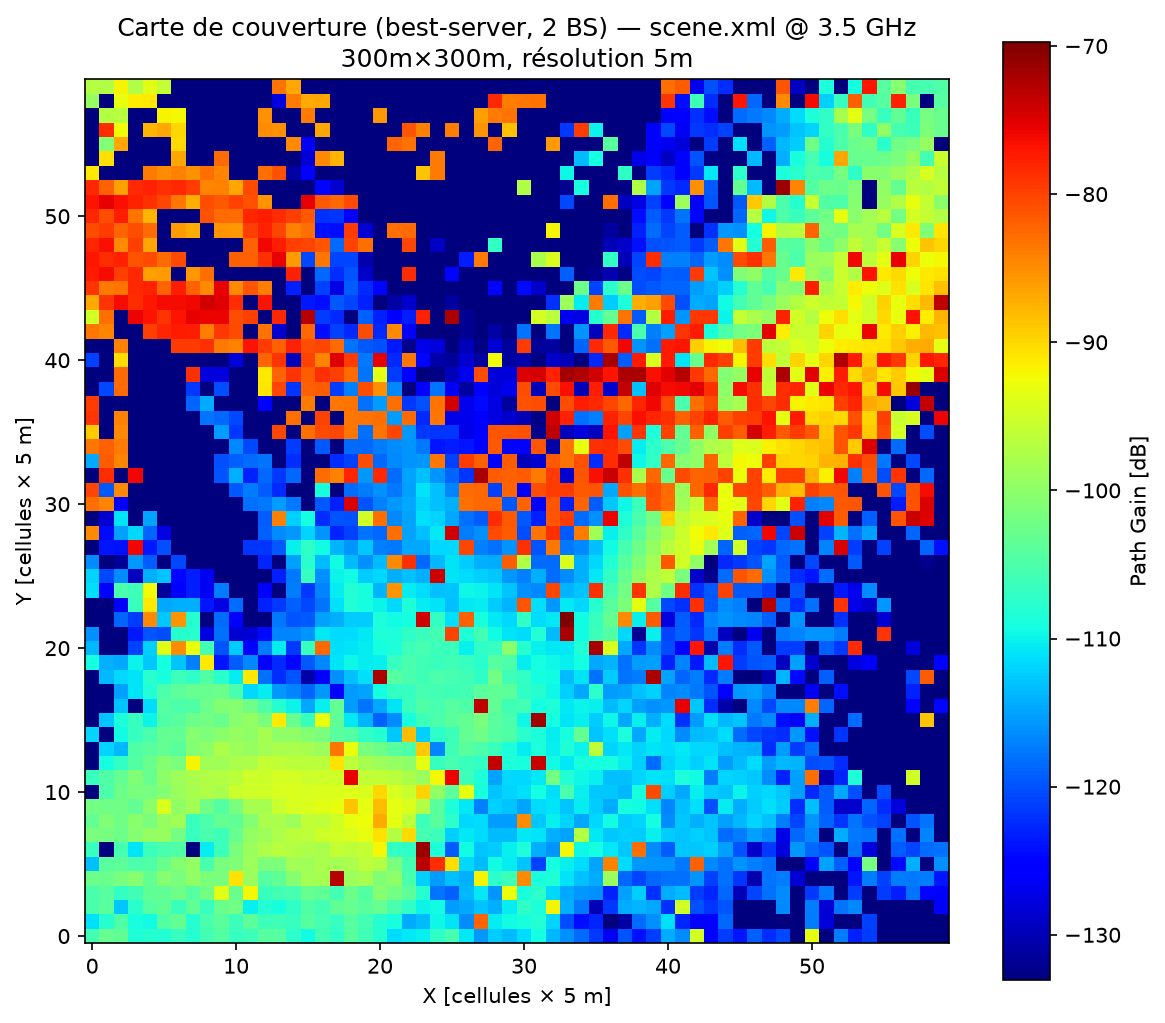
\includegraphics[width=0.75\textwidth]{radio_map_scene.png}
    \caption{Carte de couverture radio de la scène \texttt{scene.xml}.}
    \label{fig:radio_map}
\end{figure}

\begin{figure}[H]
    \centering
    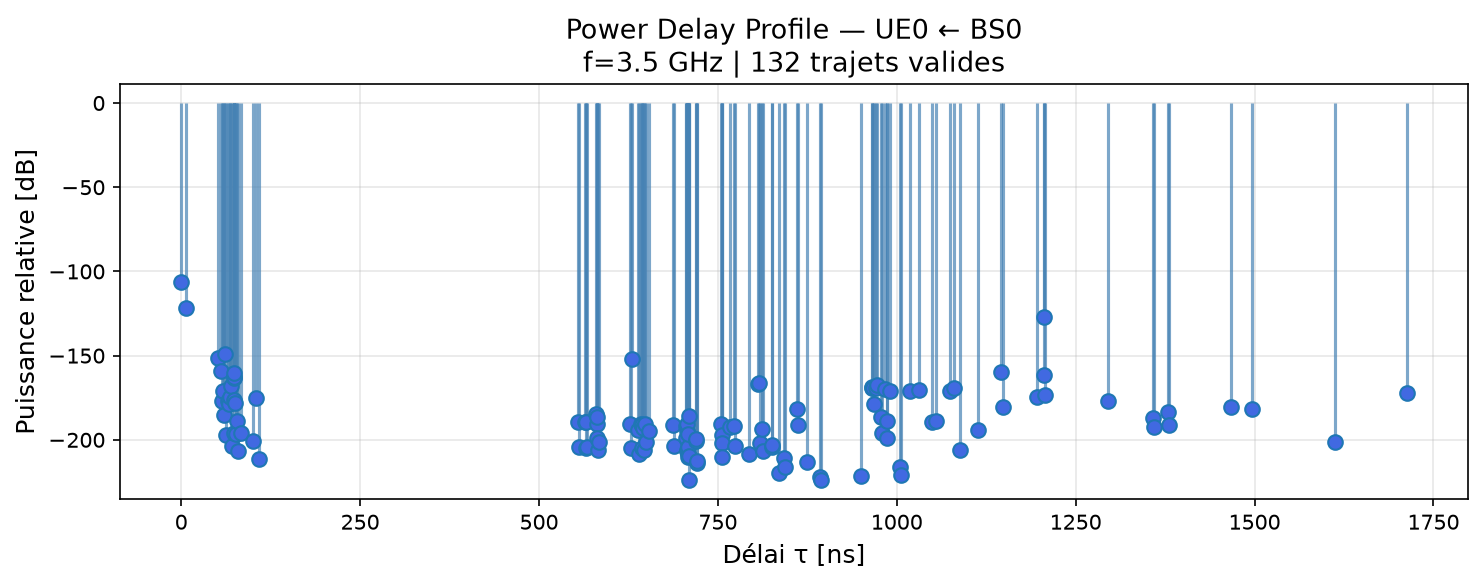
\includegraphics[width=0.48\textwidth]{pdp_ue0_bs0.png}
    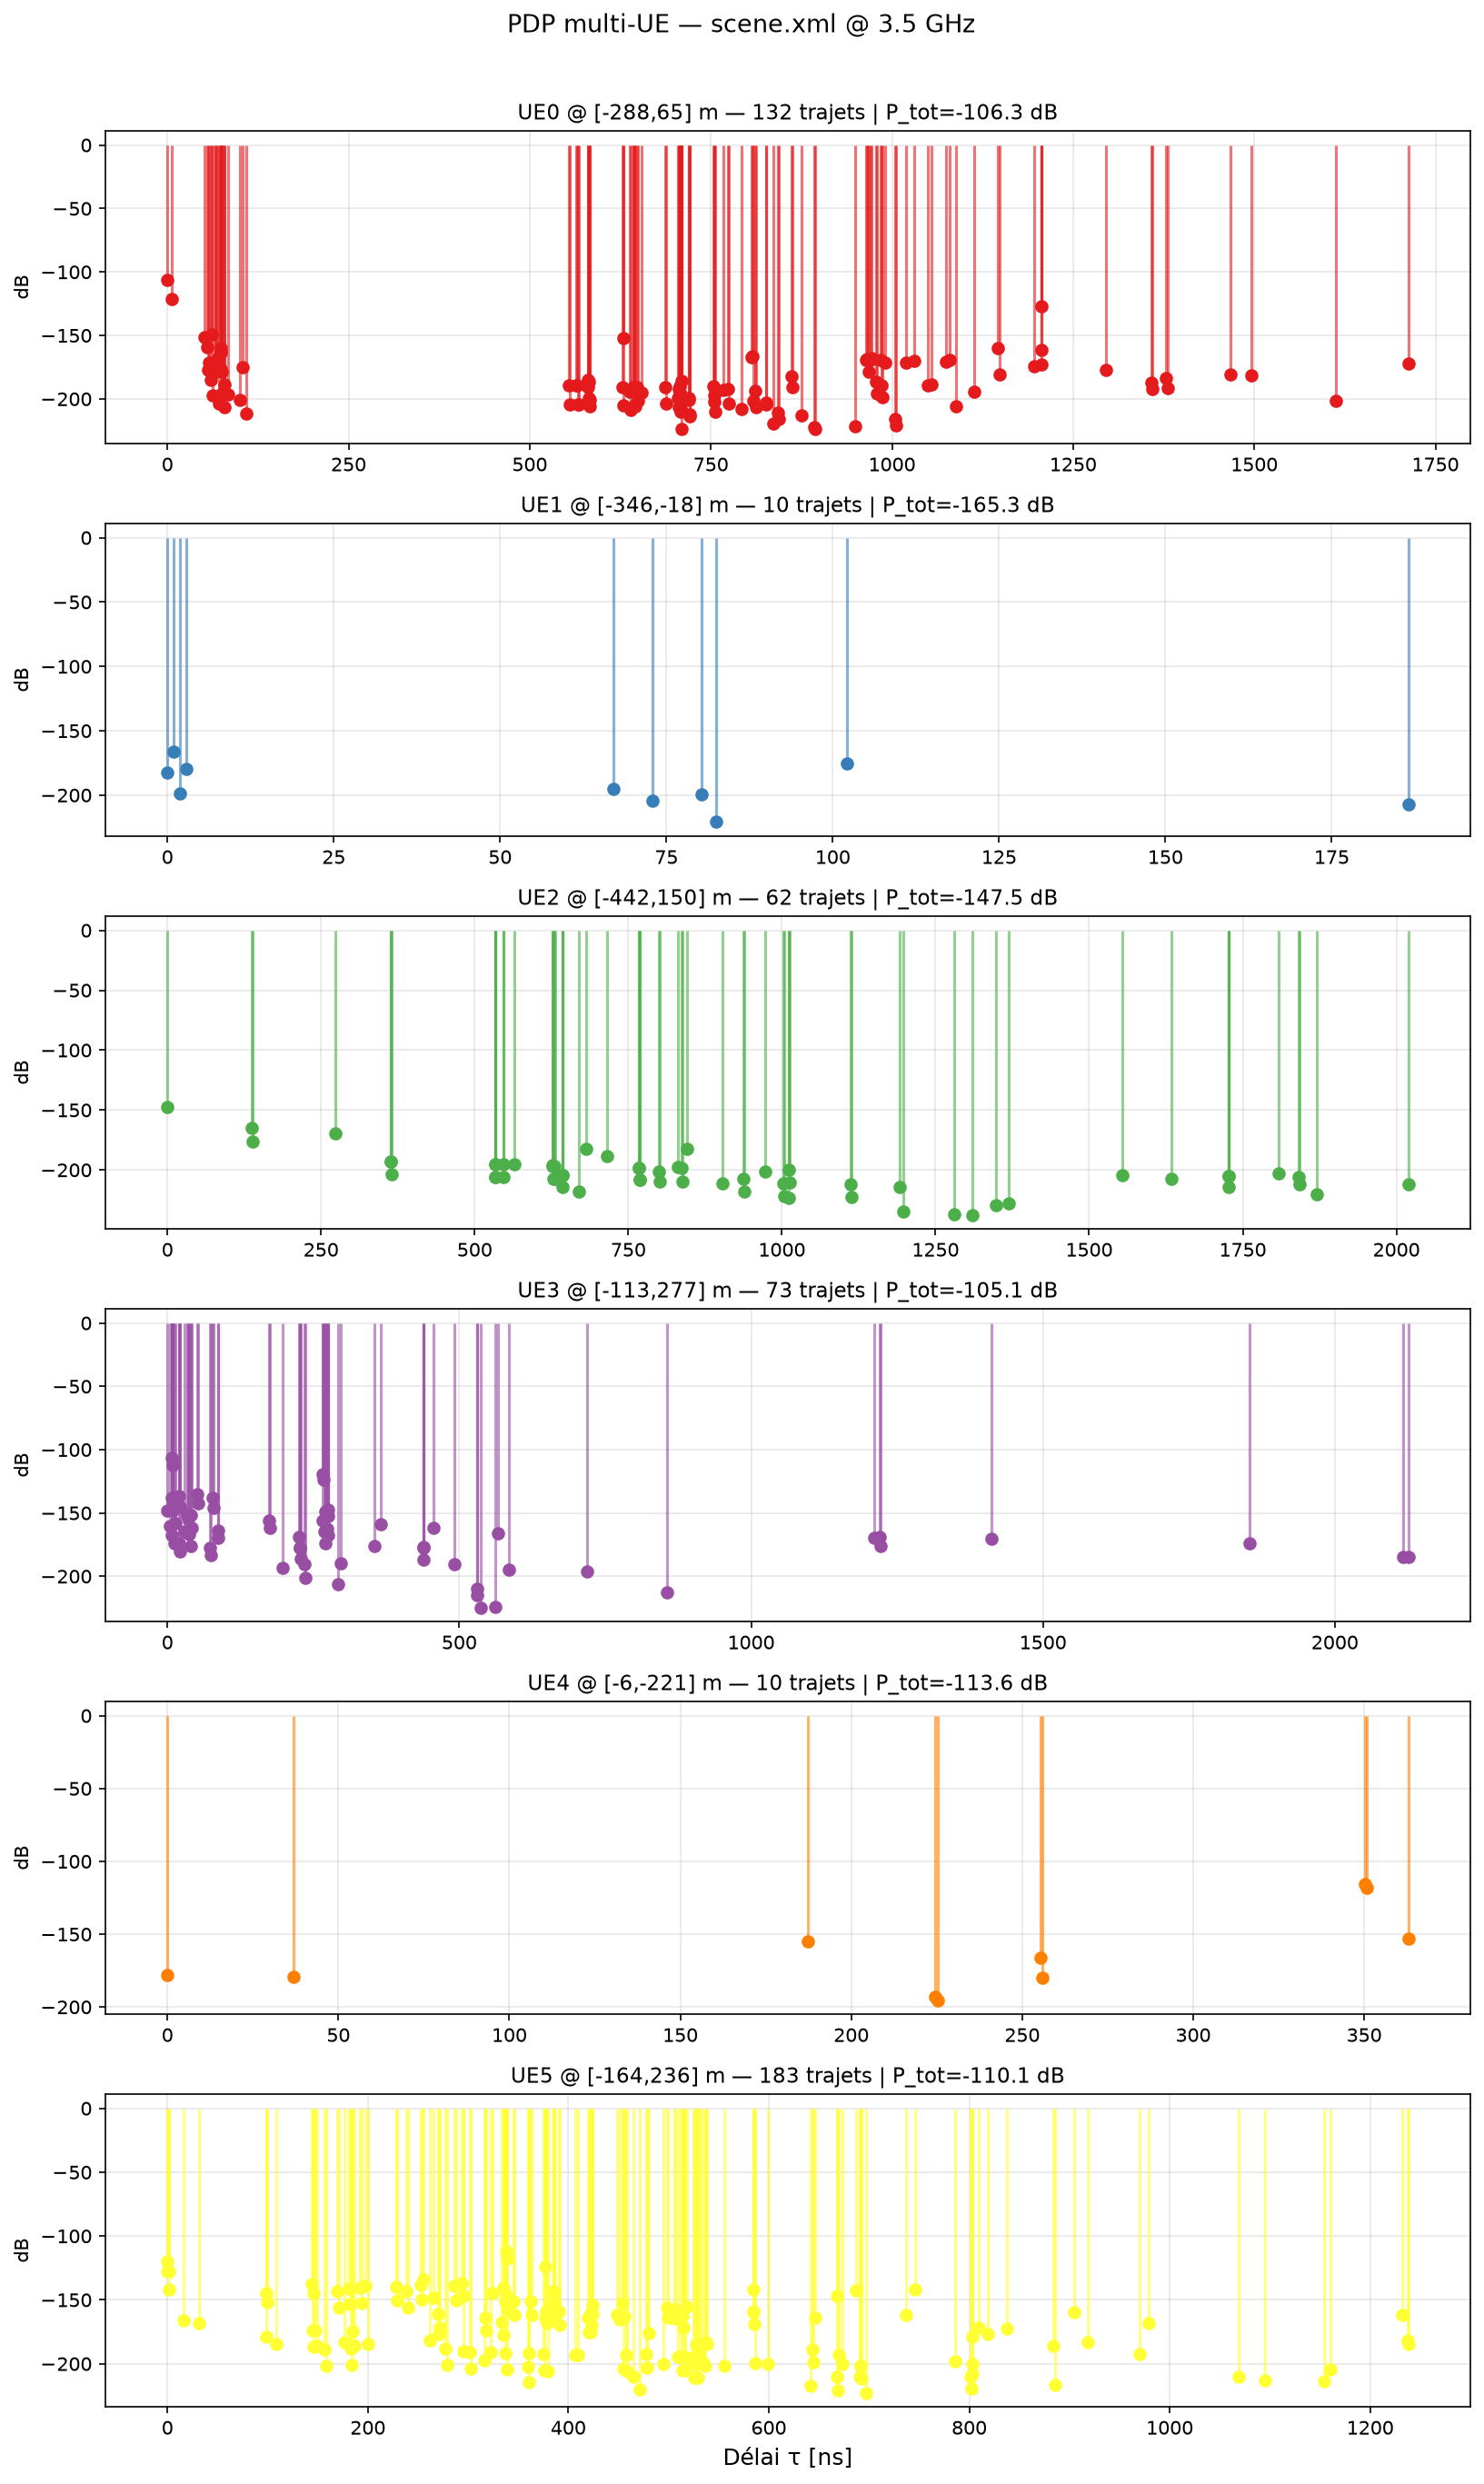
\includegraphics[width=0.48\textwidth]{pdp_all_ue.png}
    \caption{Profil de délai de puissance pour la liaison ue0--bs0 (gauche) et comparaison sur l'ensemble des UE (droite).}
    \label{fig:pdp}
\end{figure}

\subsection{Résultats de perception multimodale (modules 1b et 2)}
\label{subsec:res_phase3}

\begin{table}[H]
    \centering
    \caption{Résultats de fusion à 28~GHz, architecture finale à 4 n\oe uds BS + 2 capteurs piétons.}
    \begin{tabular}{lc}
        \toprule
        \rowcolor{tabhead}
        \hd{Indicateur} & \hd{Valeur} \\
        \midrule
        Points radar détectés (au-dessus du seuil) & 16\,784 \\
        \quad dont façade & 13\,819 \\
        \quad dont sol & 2\,628 \\
        \quad dont cible générique (\texttt{target}, avant fusion) & 337 \\
        Points étiquetés \texttt{car} par la vision & 305 \\
        Points étiquetés \texttt{pedestrian} par la vision & 32 \\
        Taux d'étiquetage des points \texttt{target} & $100\,\%$ (337/337) \\
        Contamination de points statiques par la vision & $0$ \\
        mAP50 (YOLOv8n fine-tuné) & $0{,}965$ \\
        mAP50-95 (YOLOv8n fine-tuné) & $0{,}887$ \\
        \bottomrule
    \end{tabular}
\end{table}

Sur 20\,896 points d'interaction calculés, 4\,112 (20\,\%) restent sous le seuil de détection. Le radar garde 305 points sur la voiture et 32 sur les piétons : avec une surface équivalente radar d'environ 0,5~m$^2$, contre plusieurs m$^2$ pour une voiture, un piéton renvoie près de dix fois moins d'échos détectables. Les caméras, elles, voient toujours les deux piétons (tableau~\ref{tab:res_dynamic}).

Trois chiffres du tableau demandent un peu de recul. Le \textbf{taux d'étiquetage de 100\,\%} signifie que chaque point \texttt{target} tombe dans une boîte YOLO d'au moins une caméra : les cibles radar sont toujours couvertes par la vision, ce qui justifie les six caméras. L'\textbf{absence de contamination} des points statiques découle de la règle de fusion elle-même, puisque la vision ne peut étiqueter que les points \texttt{target} ; ce n'est pas une performance, mais la preuve que cette règle fonctionne. Enfin, le \textbf{mAP50 de 0,965} est mesuré sur des rendus du même style que ceux de l'entraînement : il valide le fine-tuning dans le domaine synthétique, sans rien dire des performances sur des images réelles.

\subsubsection{Deux versions : 3,5~GHz et 28~GHz}

À partir de la phase~3, nous avons exécuté le pipeline à 3,5~GHz et à 28~GHz (\S\ref{subsec:choix_bande}). Le tableau~\ref{tab:freq_compare} et la figure~\ref{fig:chart_freq} comparent ces deux versions et la version initiale du projet :
\begin{itemize}[leftmargin=1.5em]
    \item \textbf{version initiale} : 3,5~GHz, bande de 20~MHz, \textbf{sans} seuil de détection : tout trajet valide devient un point radar, quelle que soit sa puissance ;
    \item \textbf{3,5~GHz avec seuil} : la phase~3 relancée à 3,5~GHz avec exactement la méthode actuelle (même scène, mêmes n\oe uds, même bilan de liaison avec les paramètres FR1), ce qui isole l'effet de la fréquence ;
    \item \textbf{28~GHz avec seuil} : la version détaillée dans ce rapport.
\end{itemize}
Les deux premières colonnes montrent l'effet du seuil seul ; les deux dernières, celui de la fréquence seule.

\begin{table}[H]
    \centering
    \caption{Version initiale (3,5~GHz sans seuil) et effet de la fréquence à méthode identique (seuil du tableau~\ref{tab:bilan_liaison}).}
    \label{tab:freq_compare}
    \begin{tabular}{lcccc}
        \toprule
        \rowcolor{tabhead}
        \hd{Indicateur} & \hd{\shortstack{3,5~GHz\\sans seuil}} & \hd{\shortstack{3,5~GHz\\avec seuil}} & \hd{\shortstack{28~GHz\\avec seuil}} & \hd{\shortstack{Écart\\3,5 $\to$ 28}} \\
        \midrule
        Points radar détectés & 20\,899 & 20\,481 & 16\,784 & $-18\,\%$ \\
        \quad dont façade & 17\,427 & 17\,030 & 13\,819 & $-19\,\%$ \\
        \quad dont sol & 3\,119 & 3\,099 & 2\,628 & $-15\,\%$ \\
        \quad dont cibles (\texttt{target}) & 353 & 352 & 337 & $-4\,\%$ \\
        Points étiquetés \texttt{car} & 315 & 315 & 305 & $-3\,\%$ \\
        Points étiquetés \texttt{pedestrian} & 37 & 37 & 32 & $-14\,\%$ \\
        Taux d'étiquetage des cibles & $100\,\%$ & $100\,\%$ & $100\,\%$ & $=$ \\
        Détections vision (6 caméras) & 7 & 7 & 7 & $=$ \\
        \bottomrule
    \end{tabular}
\end{table}

\begin{figure}[H]
    \centering
    \begin{tikzpicture}
    \begin{axis}[
        rapport,
        ybar, bar width=22pt,
        width=0.85\textwidth, height=6.5cm,
        symbolic x coords={Cibles,Voiture,Pietons},
        xtick=data,
        xticklabels={Cibles détectées,Points voiture,Points piétons},
        ymin=0, ymax=420,
        ylabel={Points radar},
        legend style={at={(0.5,1.02)}, anchor=south, legend columns=-1},
        enlarge x limits=0.3,
        nodes near coords, nodes near coords style={font=\small},
    ]
    \addplot[fill=white, draw=cAltB!80!black, area legend] coordinates {(Cibles,353)(Voiture,315)(Pietons,37)};
    \addplot[altB] coordinates {(Cibles,352)(Voiture,315)(Pietons,37)};
    \addplot[choix] coordinates {(Cibles,337)(Voiture,305)(Pietons,32)};
    \legend{{3,5~GHz sans seuil (version initiale)}, {3,5~GHz avec seuil}, {28~GHz avec seuil}}
    \end{axis}
    \end{tikzpicture}
    \caption{Points radar retenus sur les acteurs dans les trois configurations du tableau~\ref{tab:freq_compare}. Les deux versions à 3,5~GHz sont presque identiques : à cette fréquence, le seuil ne retire presque rien.}
    \label{fig:chart_freq}
\end{figure}

\begin{figure}[H]
    \centering
    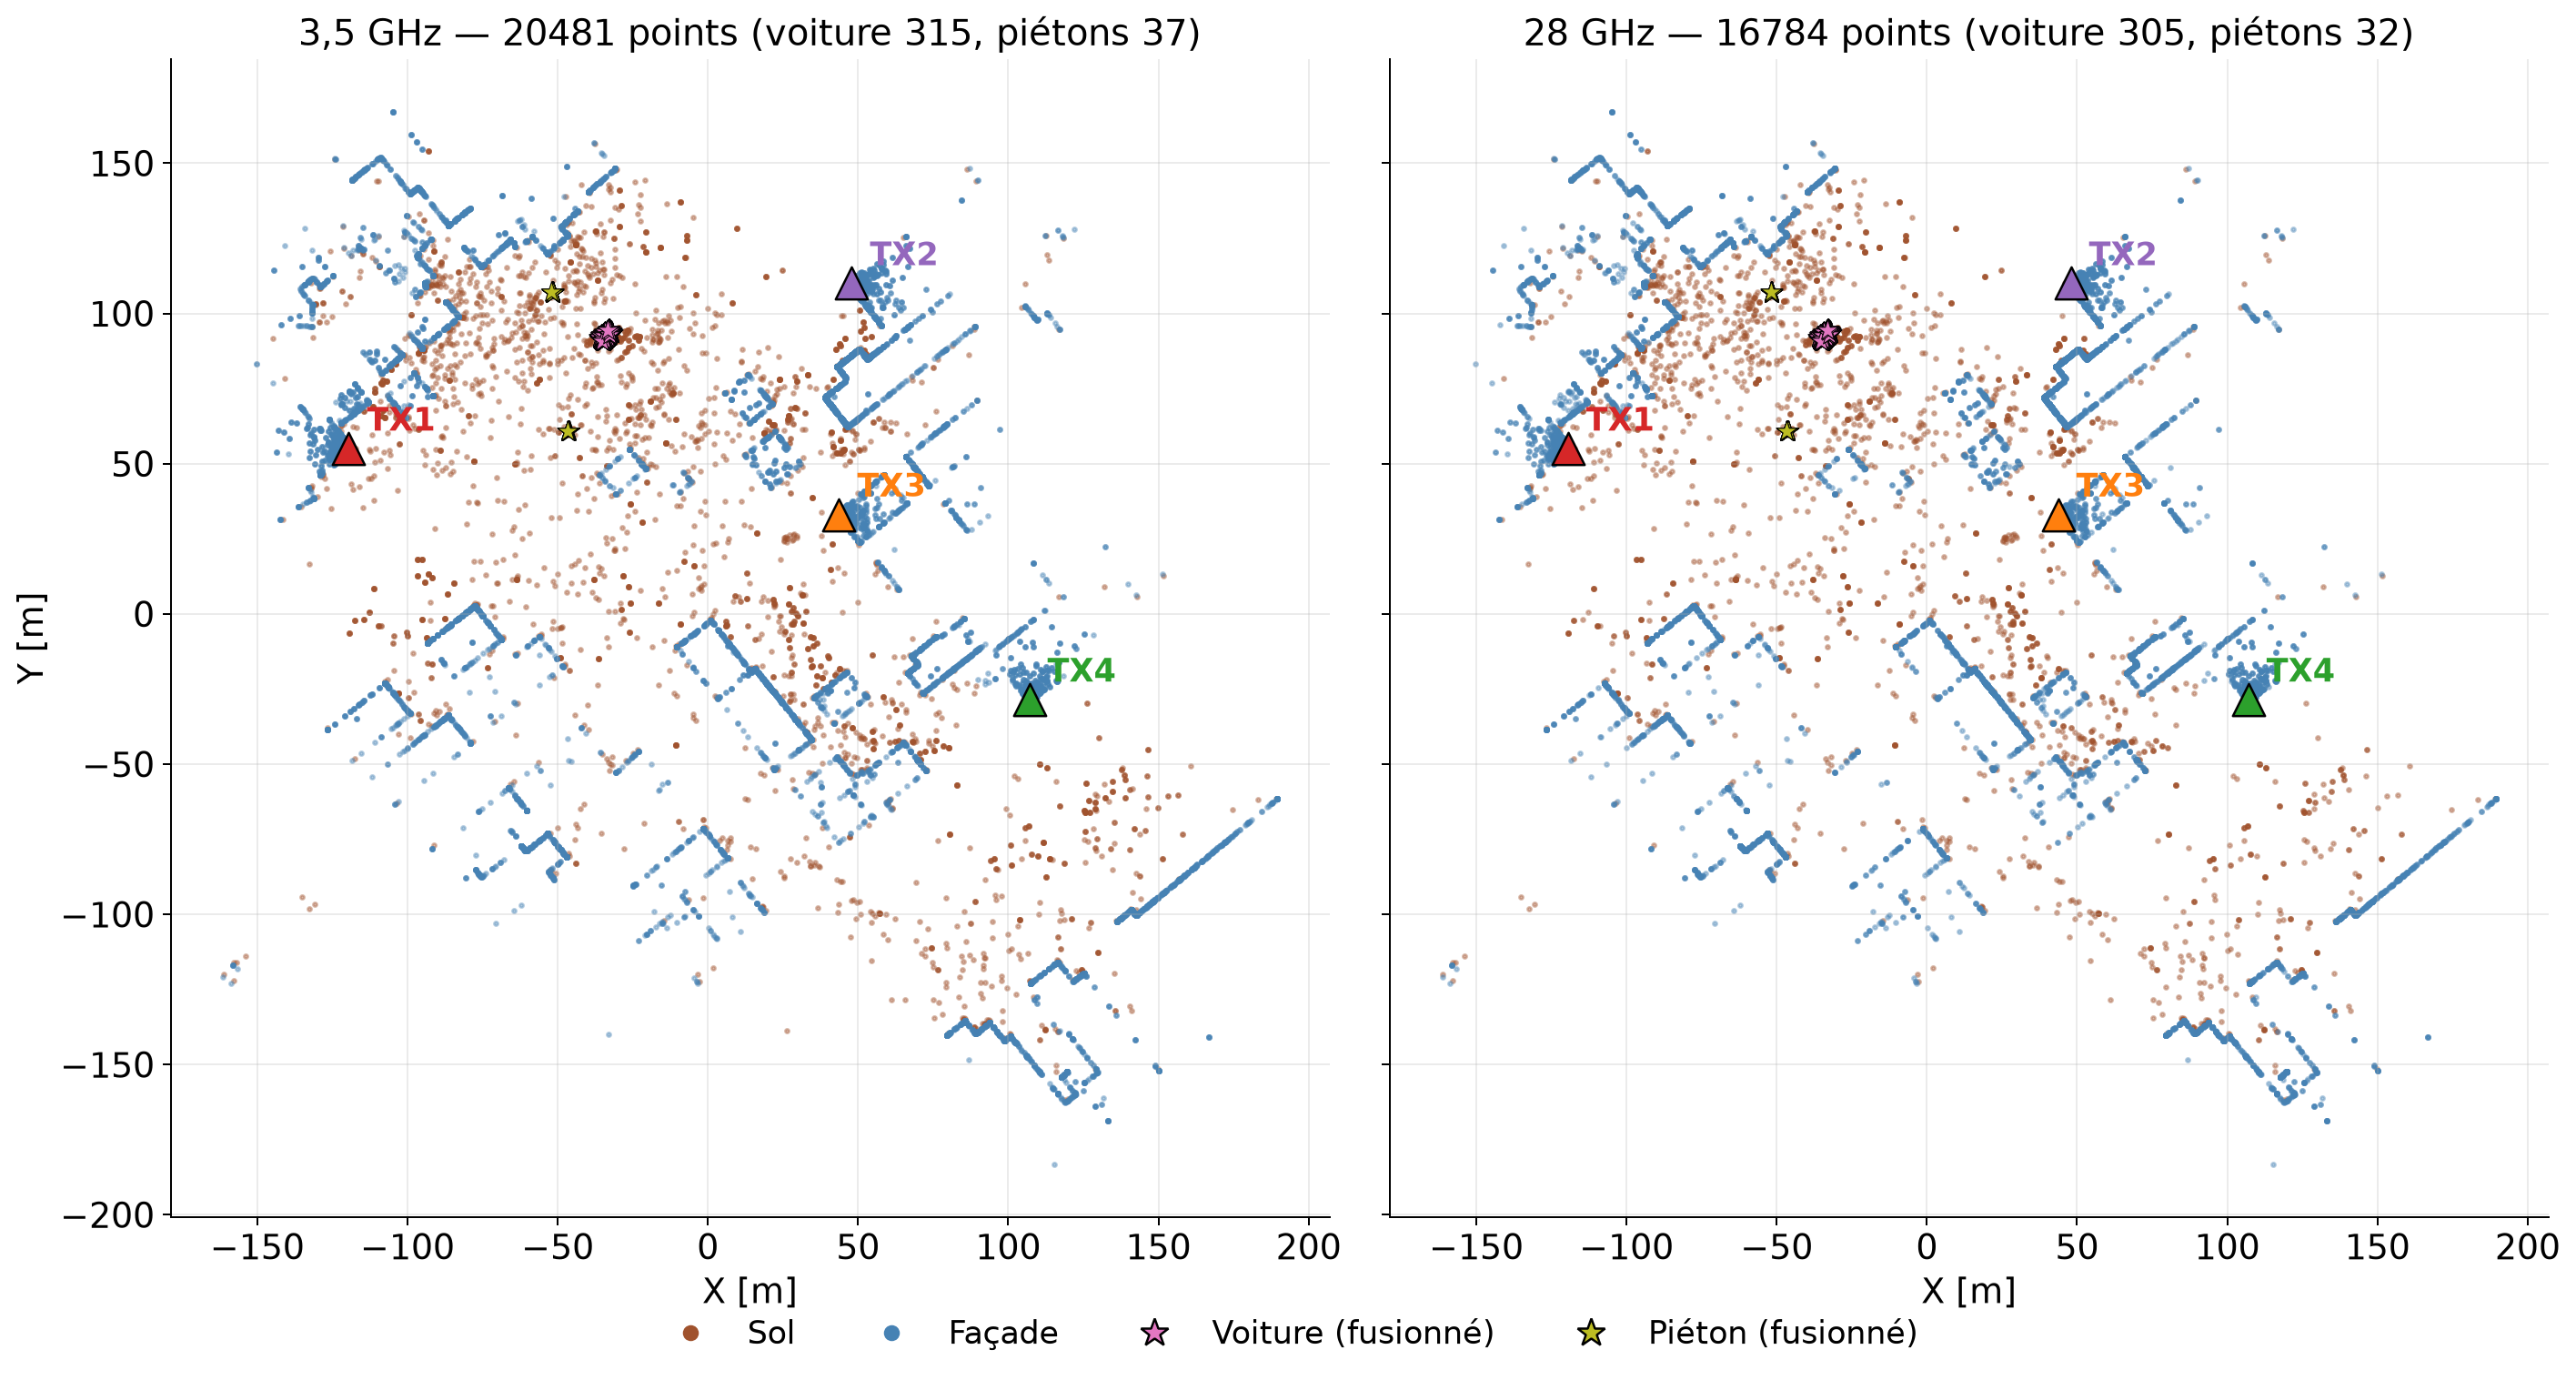
\includegraphics[width=\textwidth]{phase3/module1a_topview_3p5_vs_28GHz.png}
    \caption{Nuages de points radar retenus (vue de dessus) à 3,5~GHz et à 28~GHz, avec le même seuil de détection. À 28~GHz, ce sont surtout des points de sol et de façades éloignées qui disparaissent ; les acteurs restent détectés (305 points sur la voiture, 32 sur les piétons).}
    \label{fig:freq_topview}
\end{figure}

À 3,5~GHz, le seuil ne retire que 2\,\% des points de la version initiale (20\,899 $\to$ 20\,481) : avec un bilan de liaison réaliste, presque tous les trajets calculés jusqu'à quatre rebonds restent détectables. À méthode identique, passer à 28~GHz retire 18\,\% des points (figure~\ref{fig:freq_topview}). Le bilan l'explique. Avec des éléments d'antenne dont la surface varie comme $\lambda^2$, le gain d'un trajet entre éléments isotropes baisse de $20\log_{10}(8) \approx 18$~dB quand la fréquence est multipliée par huit, et le seuil de FR2 est 3~dB plus haut, bien que ses gains de réseaux (+12~dB) et de traitement (+6~dB) y soient déjà comptés. FR2 dispose donc d'environ 21~dB de marge en moins, et ce sont les trajets les plus faibles qui disparaissent : longs, à plusieurs rebonds, vers le sol et des façades éloignées. Les acteurs, proches des n\oe uds et en ligne de vue, sont beaucoup moins touchés ($-3\,\%$ pour la voiture, $-14\,\%$ pour les piétons, dont l'écho plus faible est plus proche du seuil). La vision ne dépend pas de la fréquence, et le taux d'étiquetage reste de 100\,\%. Les résultats à 3,5~GHz sont dans \texttt{phase3/comparaison\_3p5GHz/}.

\textbf{TX3} se comporte comme TX1 et TX2 : sa caméra détecte bien les acteurs. \textbf{TX4}, le n\oe ud le plus éloigné (180 à 210~m des acteurs), n'obtient \textbf{aucune détection vision} sur toute la séquence : un bâtiment au premier plan masque sa caméra, comme le confirme son rendu. Il contribue en revanche bien au nuage de points radar (figure~\ref{fig:radar_pointcloud}, 3\,622 points issus de TX4). Nous avons choisi de garder ce cas tel quel plutôt que de déplacer la caméra : un site réel n'offre pas toujours une vue dégagée sur toutes les cibles, et TX4 apporte toujours de la diversité au radar multistatique.

\begin{figure}[H]
    \centering
    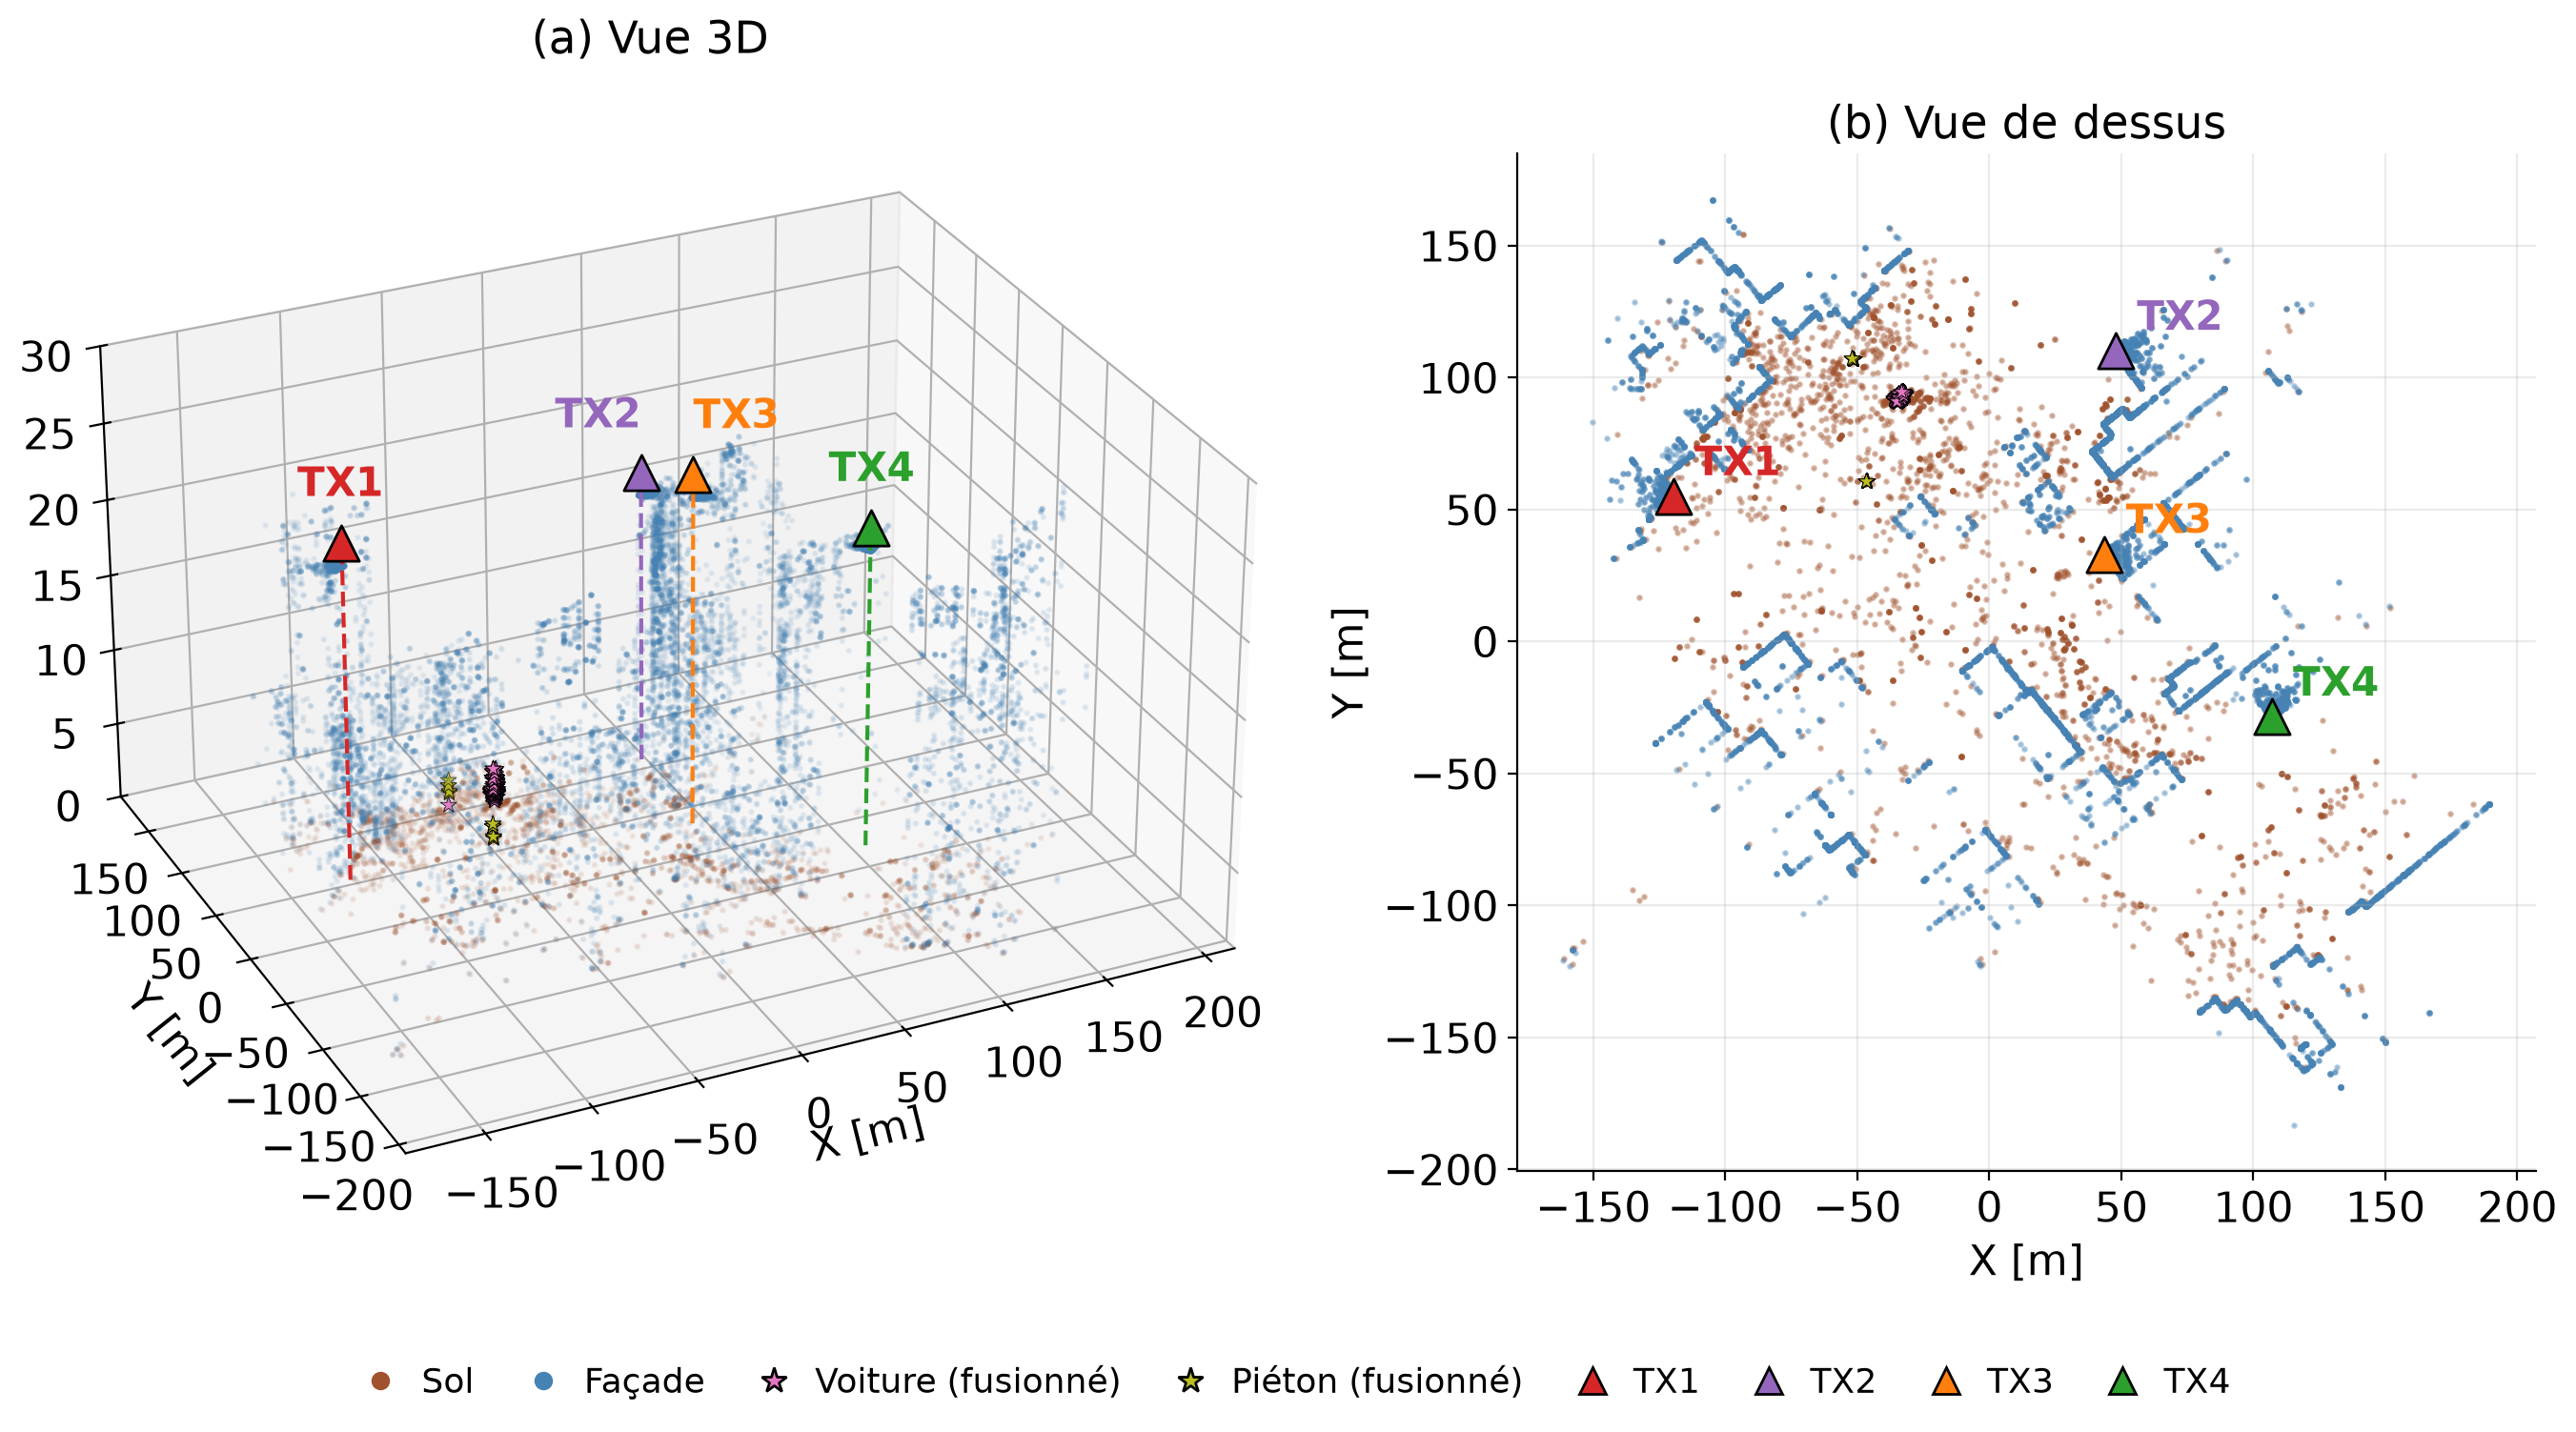
\includegraphics[width=\textwidth]{phase3/module1a_radar_pointcloud_28GHz.png}
    \caption{Nuage de points radar multistatique des 4 n\oe uds BS à 28~GHz, après seuil de détection : (a) vue 3D, les pointillés figurant le mât de chaque n\oe ud ; (b) vue de dessus. Les points \texttt{target} apparaissent avec la classe reçue lors de la fusion (voiture, piéton).}
    \label{fig:radar_pointcloud}
\end{figure}

\subsubsection{Comportement sur la séquence dynamique (6 images)}

La séquence dynamique (voiture à 1,5~m par image, piétons à 0,8~m, 6 images) permet de vérifier que la fusion reste stable dans le temps. Le tableau~\ref{tab:res_dynamic} et la figure~\ref{fig:chart_dynamic} donnent, image par image, le nombre de détections vision par n\oe ud et le nombre de points radar étiquetés par la vision.

\begin{table}[H]
    \centering
    \caption{Détections vision par n\oe ud et par image (\texttt{phase3\_dynamic\_summary\_v2.json}).}
    \label{tab:res_dynamic}
    \begin{tabular}{lcccccc}
        \toprule
        \rowcolor{tabhead}
        \hd{Image} & \hd{TX1} & \hd{TX2} & \hd{TX3} & \hd{TX4} & \hd{ped\_a} & \hd{ped\_b} \\
        \midrule
        0 & 1 & 1 & 1 & 0 & 2 & 2 \\
        1 & 1 & 2 & 1 & 0 & 2 & 2 \\
        2 & 1 & 3 & 1 & 0 & 2 & 2 \\
        3 & 1 & 4 & 2 & 0 & 2 & 2 \\
        4 & 3 & 3 & 2 & 0 & 2 & 2 \\
        5 & 3 & 3 & 3 & 0 & 2 & 2 \\
        \bottomrule
    \end{tabular}
\end{table}

\begin{figure}[H]
    \centering
    \begin{tikzpicture}
    \begin{axis}[
        rapport,
        width=0.9\textwidth, height=6.5cm,
        xlabel={Image}, ylabel={Points radar étiquetés par la vision},
        xtick={0,1,2,3,4,5},
        ymin=0, ymax=420,
        enlarge x limits=0.05,
        legend pos=south east,
        legend style={draw=gray!50, fill=white, fill opacity=0.9, text opacity=1},
    ]
    \addplot[color=cChoix, very thick, mark=*, mark options={fill=white, line width=1pt},
             nodes near coords, nodes near coords style={font=\small, color=cChoix, anchor=south, yshift=2pt}]
        coordinates {(0,337)(1,315)(2,316)(3,312)(4,314)(5,376)};
    \legend{Points étiquetés (\texttt{vision\_matched})}
    \end{axis}
    \end{tikzpicture}
    \caption{Nombre de points radar étiquetés par la vision sur les 6 images de la séquence (28~GHz). La fusion fonctionne à chaque image ; l'occultation de TX4 (aucune détection) se lit dans le tableau~\ref{tab:res_dynamic}.}
    \label{fig:chart_dynamic}
\end{figure}

Le nombre de points étiquetés varie de 312 à 376 selon l'image (figure~\ref{fig:chart_dynamic}). Ces variations viennent du radar, pas de la vision : à l'image 0, les 337 points \texttt{target} sont tous étiquetés, si bien que la courbe suit surtout le nombre d'échos des acteurs qui passent le seuil. Ce nombre dépend de la géométrie du moment (orientation de la voiture vers chaque n\oe ud, trajets diffus échantillonnés), qui change à chaque déplacement ; la hausse de la dernière image (376) correspond à la voiture qui se présente plus de face à certains n\oe uds. Côté vision, le tableau~\ref{tab:res_dynamic} montre au contraire une hausse régulière des détections des caméras en toiture (TX2 passe de 1 à 3 ou 4 détections) : en avançant vers le centre de la scène, les piétons entrent dans leur champ et deviennent assez grands pour être détectés. Les capteurs piétons, eux, détectent leurs deux cibles (piéton et voiture) à chaque image.

\subsection{Résultats de cartographie sémantique et encodage HD (module 3)}
\label{subsec:res_phase4}

La grille bayésienne 3D compte $9 \times 169 \times 179 \times 6$ cellules (Z, Y, X, classe), avec une résolution de 10~m en XY et 3~m en Z, soit $272\,259$ cellules spatiales, dont $1\,396$ sont observées à 28~GHz.

\begin{table}[H]
    \centering
    \caption{Résultats de l'encodage hyperdimensionnel.}
    \begin{tabular}{lc}
        \toprule
        \rowcolor{tabhead}
        \hd{Indicateur} & \hd{Valeur} \\
        \midrule
        Dimension de l'espace HD $D$ & $10\,000$ \\
        Niveaux par axe spatial & $64$ \\
        Ratio de compression (grille $\to$ vecteur HD) & $\times\,10\,454{,}7$ \\
        Classe retrouvée par similarité cosinus (requête position) & \texttt{car} ($0{,}380$) \\
        \bottomrule
    \end{tabular}
\end{table}

\begin{figure}[H]
    \centering
    \begin{tikzpicture}
    \begin{axis}[
        rapport,
        ybar, bar width=30pt, bar shift=0pt,
        width=0.8\textwidth, height=6.5cm,
        symbolic x coords={car,pedestrian,ground,facade},
        xtick={car,pedestrian,ground,facade},
        xticklabels={\textbf{car} (vérité terrain),pedestrian,ground,facade},
        ymin=0, ymax=0.45,
        ylabel={Similarité cosinus},
        enlarge x limits=0.18,
        nodes near coords, nodes near coords style={font=\small},
        /pgf/number format/.cd, use comma, fixed, zerofill, precision=3,
        /pgfplots/.cd, yticklabel style={/pgf/number format/.cd, zerofill=false, precision=1},
    ]
    \addplot[choix] coordinates {(car,0.380)};
    \addplot[altB] coordinates {(pedestrian,0.331)(ground,0.282)(facade,0.191)};
    \end{axis}
    \end{tikzpicture}
    \caption{Similarité cosinus de chaque classe pour une requête placée sur la voiture : la bonne classe (\texttt{car}) obtient le meilleur score, devant \texttt{pedestrian} (0,331).}
    \label{fig:chart_hd_query}
\end{figure}

Interrogée à la position de la voiture, la carte encodée renvoie bien la classe \texttt{car}, avec la similarité la plus élevée (figure~\ref{fig:chart_hd_query}). Ce résultat n'a été obtenu qu'après avoir corrigé deux pièges de capacité. D'abord, les niveaux étaient calés sur toute la scène ($\sim$1800~m), ce qui noyait le signal utile ; nous les calons maintenant sur la zone \textbf{réellement observée} ($\approx$330~m). Ensuite, en superposant toutes les cellules d'un coup, une classe nombreuse (les façades, environ 800 cellules à l'époque) écrasait une classe rare (la voiture, 1 à 3 cellules) ; nous superposons maintenant les positions \textbf{classe par classe} avant de les combiner (listing de \S\ref{sec:methodologie}).

L'écart avec les autres classes reste toutefois faible : $0{,}380$ pour \texttt{car}, contre $0{,}331$ pour \texttt{pedestrian} et $0{,}282$ pour \texttt{ground}. C'est une question de \textbf{résolution du codage}. Avec 64 niveaux sur environ 330~m, un niveau couvre à peu près 5~m, et deux niveaux voisins ne diffèrent que sur $1/128$ des composantes. Deux positions distantes de 10~m ont donc des vecteurs similaires à 0,97, et encore à 0,84 à 50~m. Les cellules des piétons, à 23 et 34~m de la voiture, et le sol qui l'entoure « répondent » ainsi presque aussi fort qu'elle. Plus de niveaux localiseraient mieux, mais le vecteur pourrait alors mémoriser moins de positions.

La compression, elle, est très forte : la grille de probabilités (environ 13~Mo en flottants 64 bits) tient dans un vecteur bipolaire de 10\,000 bits (1,22~ko), soit un facteur $10\,455$. C'est l'ordre de grandeur qu'il faut pour échanger la carte entre stations de base sur le \textit{backhaul}.

\begin{table}[H]
    \centering
    \caption{Fusion multi-BS par addition de vecteurs HD : similarité à la carte complète.}
    \begin{tabular}{lc}
        \toprule
        \rowcolor{tabhead}
        \hd{Configuration} & \hd{Similarité cosinus} \\
        \midrule
        bs2 (TX3) seul (meilleur n\oe ud individuel) & $0{,}728$ \\
        bs0 (TX1) seul & $0{,}679$ \\
        bs1 (TX2) seul & $0{,}661$ \\
        bs3 (TX4) seul & $0{,}519$ \\
        Fusion pondérée par confiance caméra (4 n\oe uds) & $0{,}587$ \\
        \bottomrule
    \end{tabular}
\end{table}

\begin{figure}[H]
    \centering
    \begin{tikzpicture}
    \begin{axis}[
        rapport,
        ybar, bar width=24pt, bar shift=0pt,
        width=\textwidth, height=6.8cm,
        symbolic x coords={bs0,bs1,bs2,bs3,Fpond},
        xtick={bs0,bs1,bs2,bs3,Fpond},
        xticklabels={bs0 (TX1),bs1 (TX2),bs2 (TX3),bs3 (TX4),Fusion pondérée},
        x tick label style={font=\small, align=center, text width=1.8cm},
        ymin=0, ymax=0.85,
        ylabel={Similarité cosinus à la carte complète},
        enlarge x limits=0.1,
        nodes near coords, nodes near coords style={font=\small},
        /pgf/number format/.cd, use comma, fixed, zerofill, precision=3,
        /pgfplots/.cd, yticklabel style={/pgf/number format/.cd, zerofill=false, precision=1},
        legend style={at={(0.5,1.02)}, anchor=south, legend columns=-1},
    ]
    \addplot[fill=cChoix!45, draw=cChoix, area legend] coordinates {(bs0,0.679)(bs1,0.661)(bs3,0.519)};
    \addplot[choix] coordinates {(bs2,0.728)};
    \addplot[altA] coordinates {(Fpond,0.587)};
    \draw[dashed, thick, cChoix] ({rel axis cs:0,0}|-{axis cs:bs2,0.728}) -- ({rel axis cs:1,0}|-{axis cs:bs2,0.728})
        node[pos=0.98, above, font=\scriptsize, anchor=south east] {meilleur n\oe ud individuel};
    \legend{N\oe ud individuel, Meilleur n\oe ud (bs2), Fusion HD (4 n\oe uds)}
    \end{axis}
    \end{tikzpicture}
    \caption{Similarité cosinus à la carte complète pour chaque n\oe ud seul et pour la fusion HD des quatre n\oe uds : le meilleur n\oe ud seul (bs2) fait mieux que la fusion.}
    \label{fig:chart_hd_fusion}
\end{figure}

Pendant le développement, avec seulement deux n\oe uds, la fusion par addition de vecteurs HD faisait mieux que chaque n\oe ud seul, ce qui validait l'idée d'une fusion multi-BS (\S\ref{subsec:pipeline_six_modules}). \textbf{Ce n'est plus vrai avec quatre n\oe uds} : la fusion pondérée ($0{,}587$) reste sous le meilleur n\oe ud seul (bs2, $0{,}728$), comme le montre la figure~\ref{fig:chart_hd_fusion}. Les similarités individuelles vont de $0{,}519$ pour TX4 à $0{,}728$ pour TX3 et suivent globalement le nombre de points radar de chaque n\oe ud : 4\,572 pour TX3, 4\,566 pour TX2, 4\,024 pour TX1 et 3\,622 pour TX4. Les deux extrêmes coïncident, mais l'ordre n'est pas strict : TX1 ($0{,}679$) passe devant TX2 ($0{,}661$) avec 542 points de moins. Ce qui compte, ce sont plutôt les \emph{cellules} couvertes : 30\,\% des points de TX2 (1\,388) sont à moins de 20~m de son mât, sur les façades voisines (figure~\ref{fig:radar_pointcloud}), si bien qu'il ne couvre que 505 cellules, contre 686 pour TX1 et 734 pour TX3. Le nombre de cellules n'explique pas tout pour autant : TX4 en couvre 585 et reste dernier, ce qui montre que la position et la classe des cellules comptent aussi. Pourquoi la fusion déçoit-elle ? Chaque vecteur de n\oe ud est déjà réduit à des valeurs bipolaires avant d'être additionné (c'est ce qui permet de le transmettre sur le \textit{backhaul}), et avec seulement 3 ou 4 vecteurs, les égalités lors du vote majoritaire deviennent fréquentes. C'est une \textbf{limite connue de la superposition bipolaire en HDC}, et non une erreur d'implémentation. Nous la documentons dans le notebook et dans \texttt{phase4\_summary.json}. Elle ne concerne que cette démonstration de compression : la grille bayésienne 3D, qui est la carte de référence, intègre correctement les six n\oe uds par mise à jour bayésienne directe, sans passer par cette étape bipolaire.

\textbf{Version à 3,5~GHz.} Comme la phase~3, la phase~4 a été exécutée à 3,5~GHz avec exactement la même méthode (\texttt{phase4/comparaison\_3p5GHz/}). Le tableau~\ref{tab:hd_compare} compare les deux versions et la version initiale du projet (3,5~GHz, sans seuil de détection).

\begin{table}[H]
    \centering
    \caption{Module 3 : version initiale (3,5~GHz sans seuil) et deux versions à seuil identique (3,5~GHz et 28~GHz).}
    \label{tab:hd_compare}
    \begin{tabularx}{\textwidth}{F{4.6cm}CCC}
        \toprule
        \rowcolor{tabhead}
        \hd{Indicateur} & \hd{\shortstack{3,5~GHz\\sans seuil}} & \hd{\shortstack{3,5~GHz\\avec seuil}} & \hd{\shortstack{28~GHz\\avec seuil}} \\
        \midrule
        Cellules observées de la grille 3D & 1\,449 & 1\,447 & 1\,396 \\
        Ratio de compression (grille $\to$ vecteur HD) & $\times\,10\,454{,}7$ & $\times\,10\,454{,}7$ & $\times\,10\,454{,}7$ \\
        Requête position $\to$ classe : \texttt{car} & $0{,}379$ & $0{,}379$ & $0{,}380$ \\
        \quad classe suivante & \texttt{pedestrian} ($0{,}332$) & \texttt{pedestrian} ($0{,}332$) & \texttt{pedestrian} ($0{,}331$) \\
        Meilleur n\oe ud individuel & bs2/TX3 ($0{,}752$) & bs2/TX3 ($0{,}752$) & bs2/TX3 ($0{,}728$) \\
        n\oe ud le plus faible (TX4) & $0{,}520$ & $0{,}516$ & $0{,}519$ \\
        Fusion pondérée (4 n\oe uds) & $0{,}597$ & $0{,}596$ & $0{,}587$ \\
        \bottomrule
    \end{tabularx}
\end{table}

Avec le bilan de liaison réaliste, la version à 3,5~GHz est presque identique à la version initiale sans seuil (1\,447 contre 1\,449 cellules), puisque le seuil n'y retire que 2\,\% des points. À bilan identique, la grille à 28~GHz ne compte que 4\,\% de cellules en moins (1\,396 contre 1\,447), alors qu'elle a perdu 18\,\% des points : la plupart des points perdus tombaient dans des cellules déjà vues grâce à d'autres trajets. La requête retrouve la voiture dans les trois versions, avec le même écart sur la classe suivante ($0{,}049$ à 28~GHz, $0{,}047$ à 3,5~GHz). Le ratio de compression ne change pas, puisqu'il dépend de la taille de la grille et non du nombre de cellules observées. Quant à la fusion HD multi-BS, la conclusion est la même partout : elle reste sous le meilleur n\oe ud seul, quelle que soit la bande.

\begin{figure}[H]
    \centering
    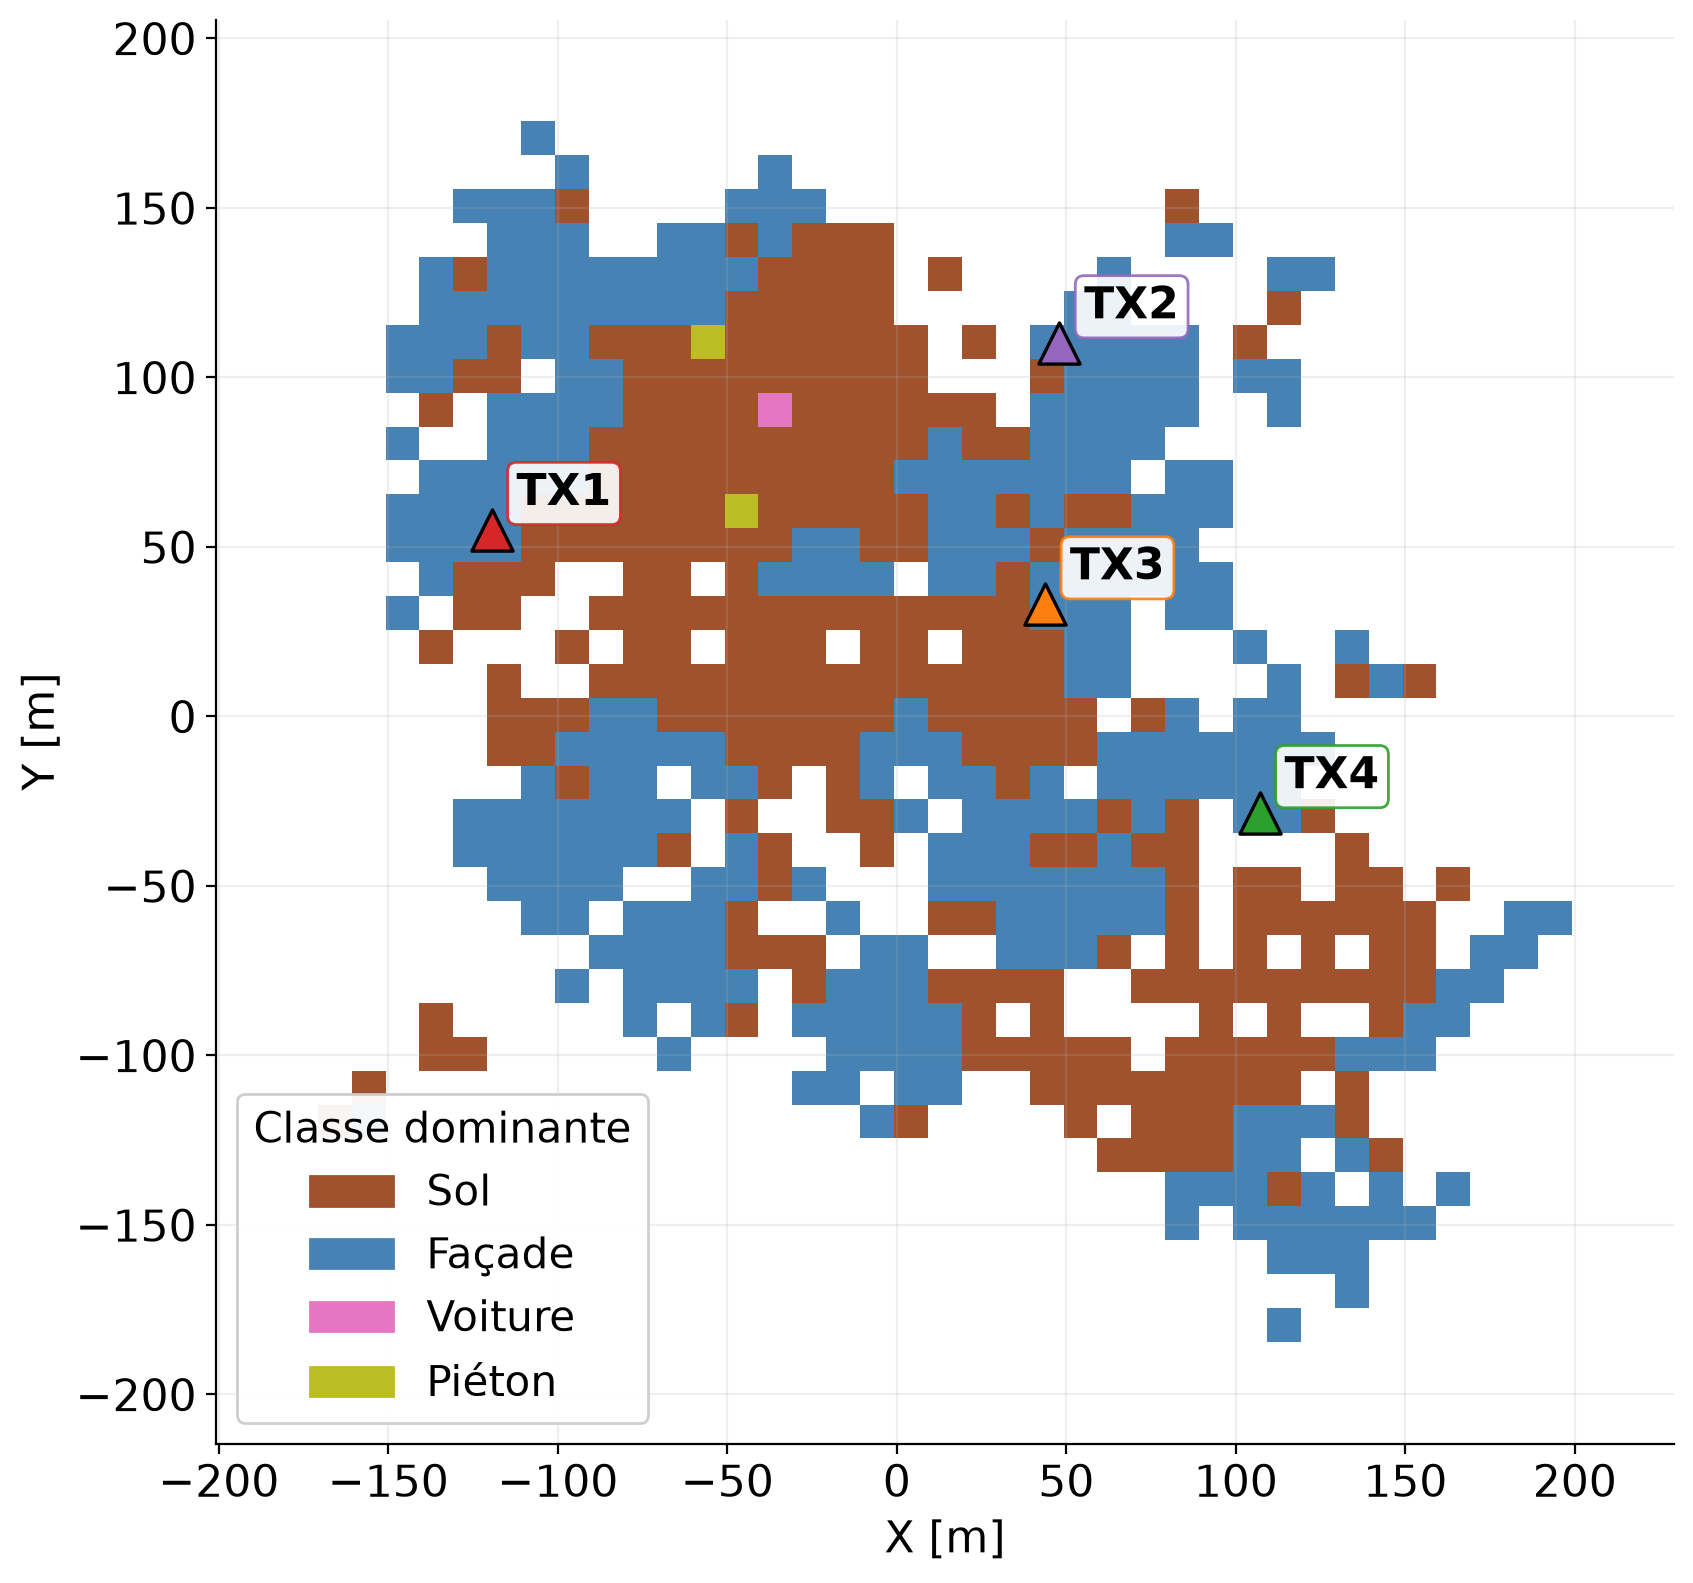
\includegraphics[width=0.82\textwidth]{phase4/module3_grid3d_topdown_28GHz.png}
    \caption{Grille bayésienne 3D à 28~GHz vue de dessus (classe dominante de chaque colonne, cellules de 10~m), recadrée sur la zone observée.}
    \label{fig:phase4_topdown}
\end{figure}

\begin{figure}[H]
    \centering
    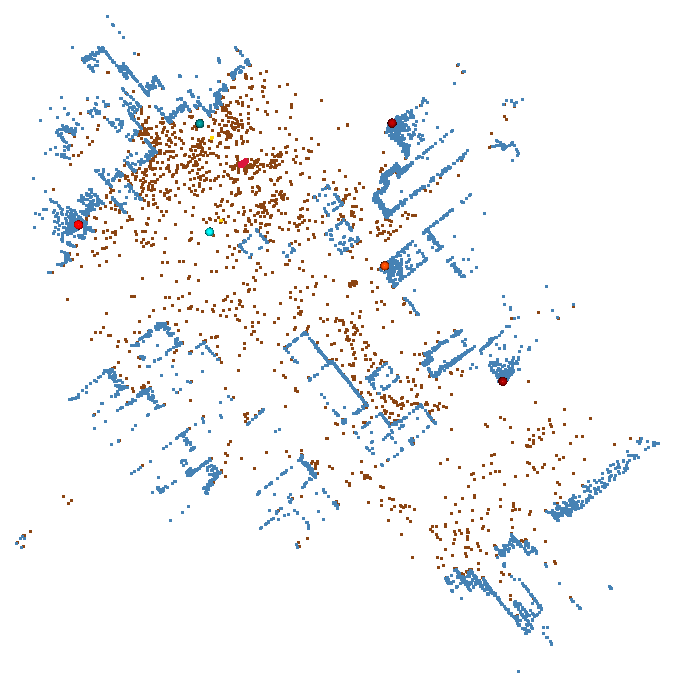
\includegraphics[width=0.82\textwidth]{phase4/module3_open3d_pointcloud_28GHz.png}
    \caption{Rendu Open3D du nuage de points sémantique coloré par classe, avec les 6 n\oe uds de sensing.}
    \label{fig:phase4_open3d}
\end{figure}

Les deux vues de la grille (figures~\ref{fig:phase4_topdown} et~\ref{fig:phase4_open3d}) illustrent ces constats. Les façades apparaissent sur toute la zone observée, plus denses autour des n\oe uds, dont les réflexions proches sont les plus fortes, et le long des grandes façades rectilignes au sud-est. Le sol couvre une large bande centrale entre les n\oe uds et les acteurs, là où convergent les trajets, ainsi qu'une zone au sud-est autour de TX4. La voiture et chaque piéton n'occupent qu'une cellule de 10~m : assez pour les situer dans la scène, pas pour décrire leur forme. C'est ce que fait la couche dynamique de la phase~5 (\S\ref{subsec:res_phase5}), qui représente les acteurs comme des objets plutôt que comme des cellules.

\subsection{Résultats du jumeau numérique double bande (phase 5)}
\label{subsec:res_phase5}

\subsubsection{Qualité des mesures radar}

Sans bruit, un écho à un rebond est replacé à 8 à 10~mm près (tableau~\ref{tab:mesures_phase5}) : la reconstruction par retard et angle d'arrivée (équation~\eqref{eq:point_apparent}) est exacte, ce qui valide le modèle de mesure. Avec bruit, FR2 localise près de cinq fois mieux que FR1 : 0,42~m contre 2,01~m pour un écho à un rebond (figure~\ref{fig:mesures_phase5}a). Comme le SNR est élevé dans les deux bandes, l'erreur d'angle est dominée par le plancher fixé au dixième de l'ouverture du réseau (1,3° en FR1, 0,6° en FR2), soit environ 2,2~m contre 1,1~m d'erreur transverse à 100~m. C'est donc la \emph{résolution angulaire}, plus que la résolution en distance, qui fait la différence.

Surtout, \textbf{FR1 ne sépare aucune cible mobile par le Doppler} (figure~\ref{fig:mesures_phase5}b). Un piéton à 1,6~m/s produit au plus $2v/\lambda \approx 37$~Hz à 3,5~GHz, sous la résolution de 100~Hz, contre environ 300~Hz à 28~GHz, où 96\,\% des échos d'acteurs sont séparables. Dans les deux bandes, environ 30\,\% des échos détectés passent par plusieurs rebonds : autant de fantômes potentiels que le jumeau doit filtrer.

\begin{table}[H]
    \centering
    \caption{Qualité des mesures radar de la phase 5 (image 0, tirage de référence).}
    \label{tab:mesures_phase5}
    \begin{tabular}{lcc}
        \toprule
        \rowcolor{tabhead}
        \hd{Indicateur} & \hd{FR1} & \hd{FR2} \\
        \midrule
        Échos détectés & 9\,339 & 7\,138 \\
        Erreur sans bruit, écho à un rebond & 10~mm & 8~mm \\
        Erreur médiane avec bruit, écho à un rebond & 2,01~m & 0,42~m \\
        Part d'échos à plusieurs rebonds (fantômes potentiels) & 27\,\% & 31\,\% \\
        $|$Doppler$|$ médian des échos sur les acteurs & 45~Hz & 357~Hz \\
        Échos d'acteurs séparables par Doppler ($\geq 100$~Hz) & 0\,\% & 96\,\% \\
        \bottomrule
    \end{tabular}
\end{table}

\begin{figure}[H]
    \centering
    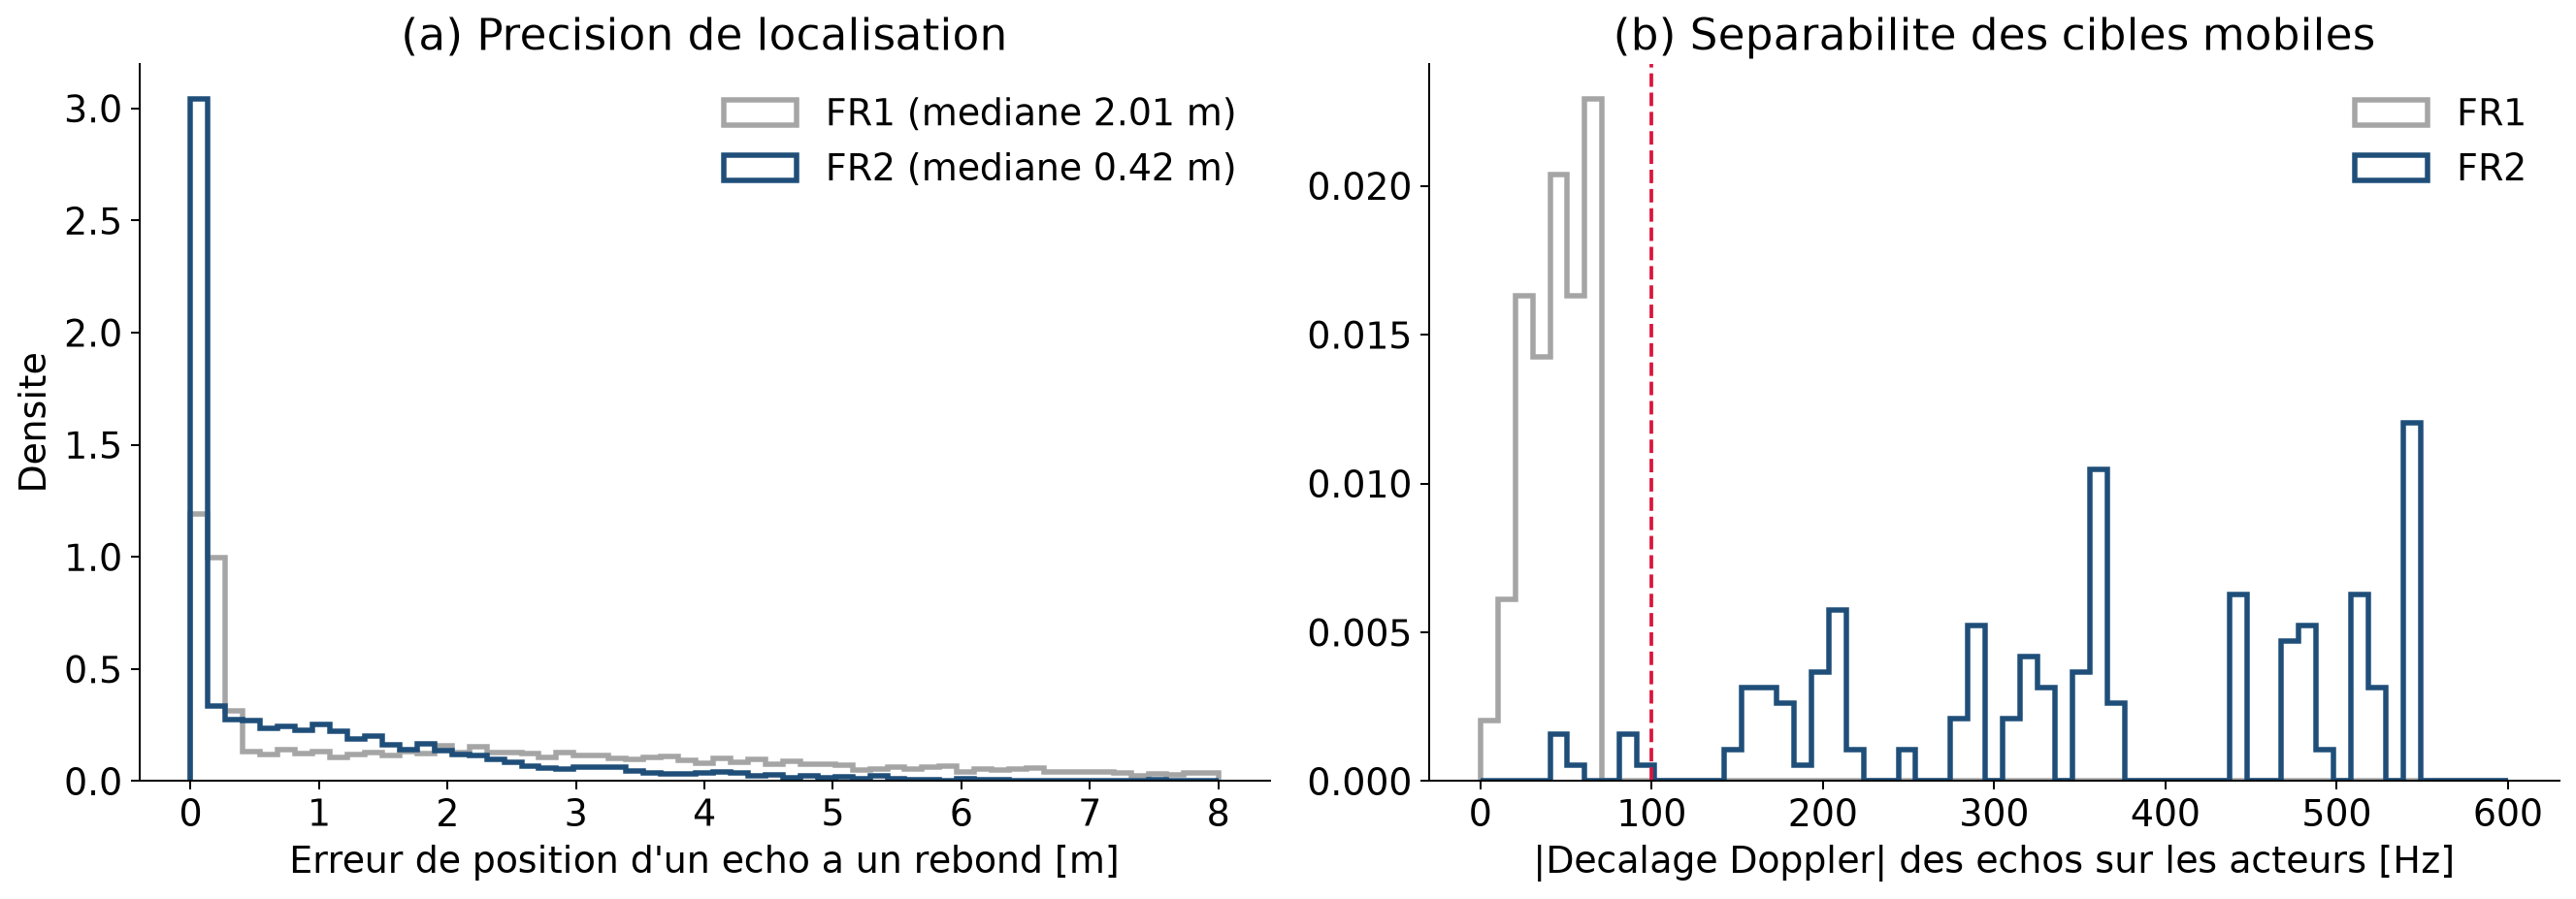
\includegraphics[width=\textwidth]{phase5/module1a_mesures_fr1_fr2.png}
    \caption{Phase 5 : (a) erreur de position des échos à un rebond en FR1 et FR2 ; (b) décalage Doppler des échos sur les acteurs, la ligne pointillée marquant la résolution Doppler de 100~Hz.}
    \label{fig:mesures_phase5}
\end{figure}

\subsubsection{Détection et reconnaissance des acteurs}

La figure~\ref{fig:camera_phase5} montre toute la chaîne sur deux caméras, à l'image 4. YOLO encadre la voiture (confiance 0,93 depuis le toit de TX1, 0,95 depuis le capteur piéton A) et les piétons (0,96 de près, 0,43 à 0,45 depuis le toit, d'où ils ne font que quelques pixels). Les échos FR2 à Doppler non nul, projetés dans l'image, se concentrent sur la voiture et prennent son étiquette. Les échos roses hors de sa boîte sont des fantômes de trajets multiples ; le filtre des points de vue les élimine, comme le montrent les croix de la figure~\ref{fig:zoom_phase5}.

\begin{figure}[H]
    \centering
    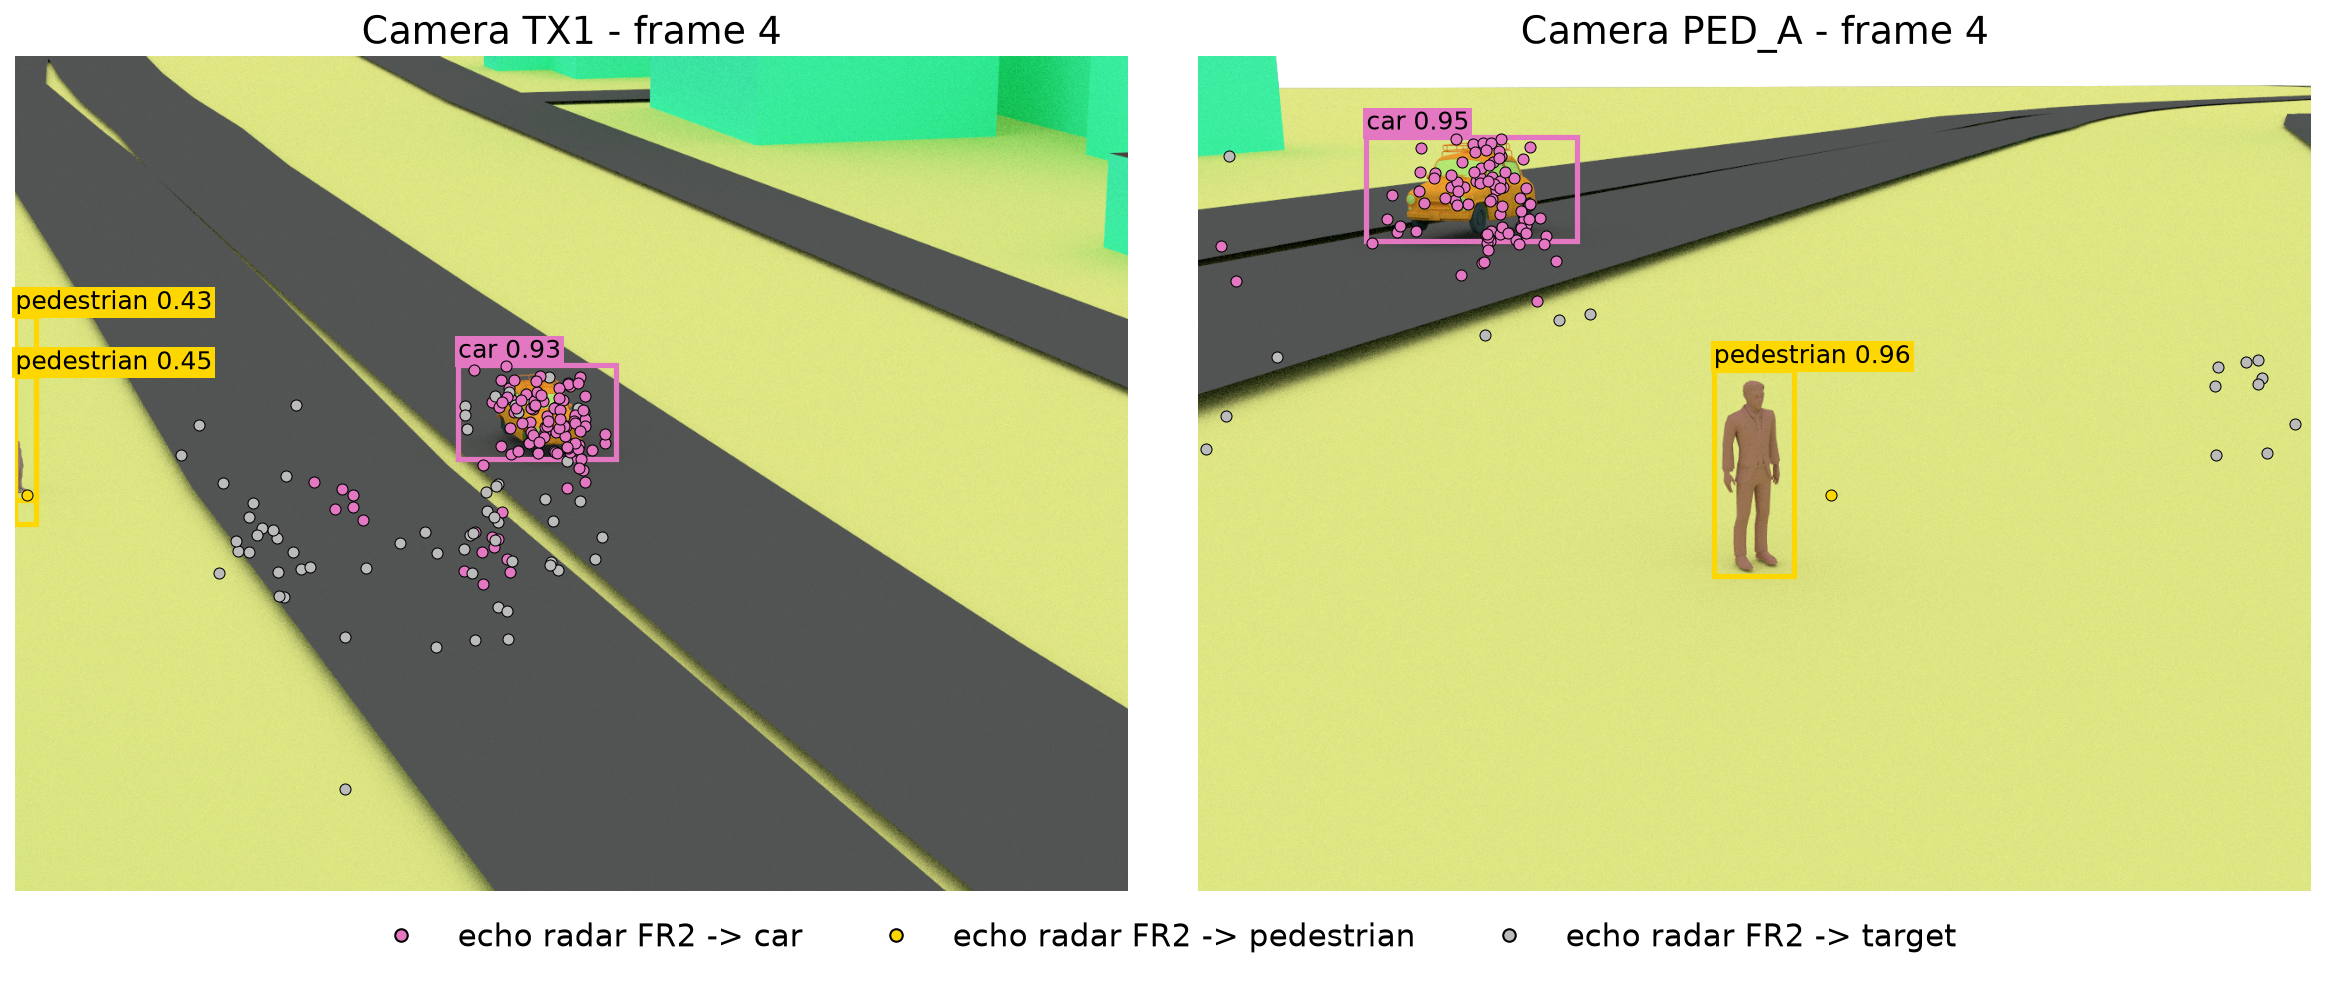
\includegraphics[width=\textwidth]{phase5/module2_reconnaissance_camera.png}
    \caption{Phase 5, image 4 : boîtes YOLO (classe et confiance) et échos radar FR2 à Doppler non nul projetés dans l'image, colorés selon la classe reçue lors de la fusion. À gauche, caméra de TX1 en toiture ; à droite, caméra du capteur piéton A.}
    \label{fig:camera_phase5}
\end{figure}

\subsubsection{Qualité du jumeau numérique}

Le tableau~\ref{tab:config_phase5} et la figure~\ref{fig:metriques_phase5} comparent les quatre configurations. La figure~\ref{fig:vues_phase5} montre la couche statique, et la figure~\ref{fig:zoom_phase5} la couche dynamique, agrandie sur la zone des acteurs.

\begin{table}[H]
    \centering
    \caption{Jumeau numérique de la phase 5 : évaluation par rapport à la vérité terrain (moyenne $\pm$ écart-type sur 10 tirages du bruit).}
    \label{tab:config_phase5}
    \begin{tabularx}{\textwidth}{F{4.2cm}CCCC}
        \toprule
        \rowcolor{tabhead}
        \hd{Indicateur} & \hd{C1 FR1} & \hd{C2 FR2} & \hd{C3 FR1+FR2} & \hd{C4 FR1+FR2 + vision} \\
        \midrule
        Structures : précision & $0{,}89 \pm 0{,}01$ & $0{,}98 \pm 0{,}00$ & $0{,}92 \pm 0{,}00$ & $0{,}92 \pm 0{,}00$ \\
        Structures : rappel & $0{,}27 \pm 0{,}01$ & $0{,}28 \pm 0{,}01$ & $0{,}36 \pm 0{,}01$ & $0{,}36 \pm 0{,}01$ \\
        Structures : F1 & $0{,}42 \pm 0{,}01$ & $0{,}44 \pm 0{,}01$ & $0{,}52 \pm 0{,}01$ & $0{,}52 \pm 0{,}01$ \\
        Sol : précision / rappel & 0,98 / 0,02 & 0,99 / 0,02 & 0,98 / 0,04 & 0,98 / 0,04 \\
        Erreur médiane des points & 0,77~m & 0,44~m & 0,57~m & 0,57~m \\
        Points à plus de 2~m de toute surface & 27\,\% & 12\,\% & 20\,\% & 20\,\% \\
        Voiture bien classée & 0\,\% & 100\,\% & 100\,\% & 100\,\% \\
        Piéton A bien classé & 0\,\% & 0\,\% & 0\,\% & $77 \pm 13$\,\% \\
        Piéton B bien classé & 0\,\% & $20 \pm 16$\,\% & $20 \pm 16$\,\% & $97 \pm 7$\,\% \\
        Erreur de position (voiture / piétons) & -- & 0,52 / 0,41~m & 0,52 / 0,41~m & 0,52 / 0,35--0,39~m \\
        Faux objets par image & 0 & $0{,}08 \pm 0{,}17$ & $0{,}08 \pm 0{,}17$ & $0{,}08 \pm 0{,}17$ \\
        \bottomrule
    \end{tabularx}
\end{table}

\begin{figure}[H]
    \centering
    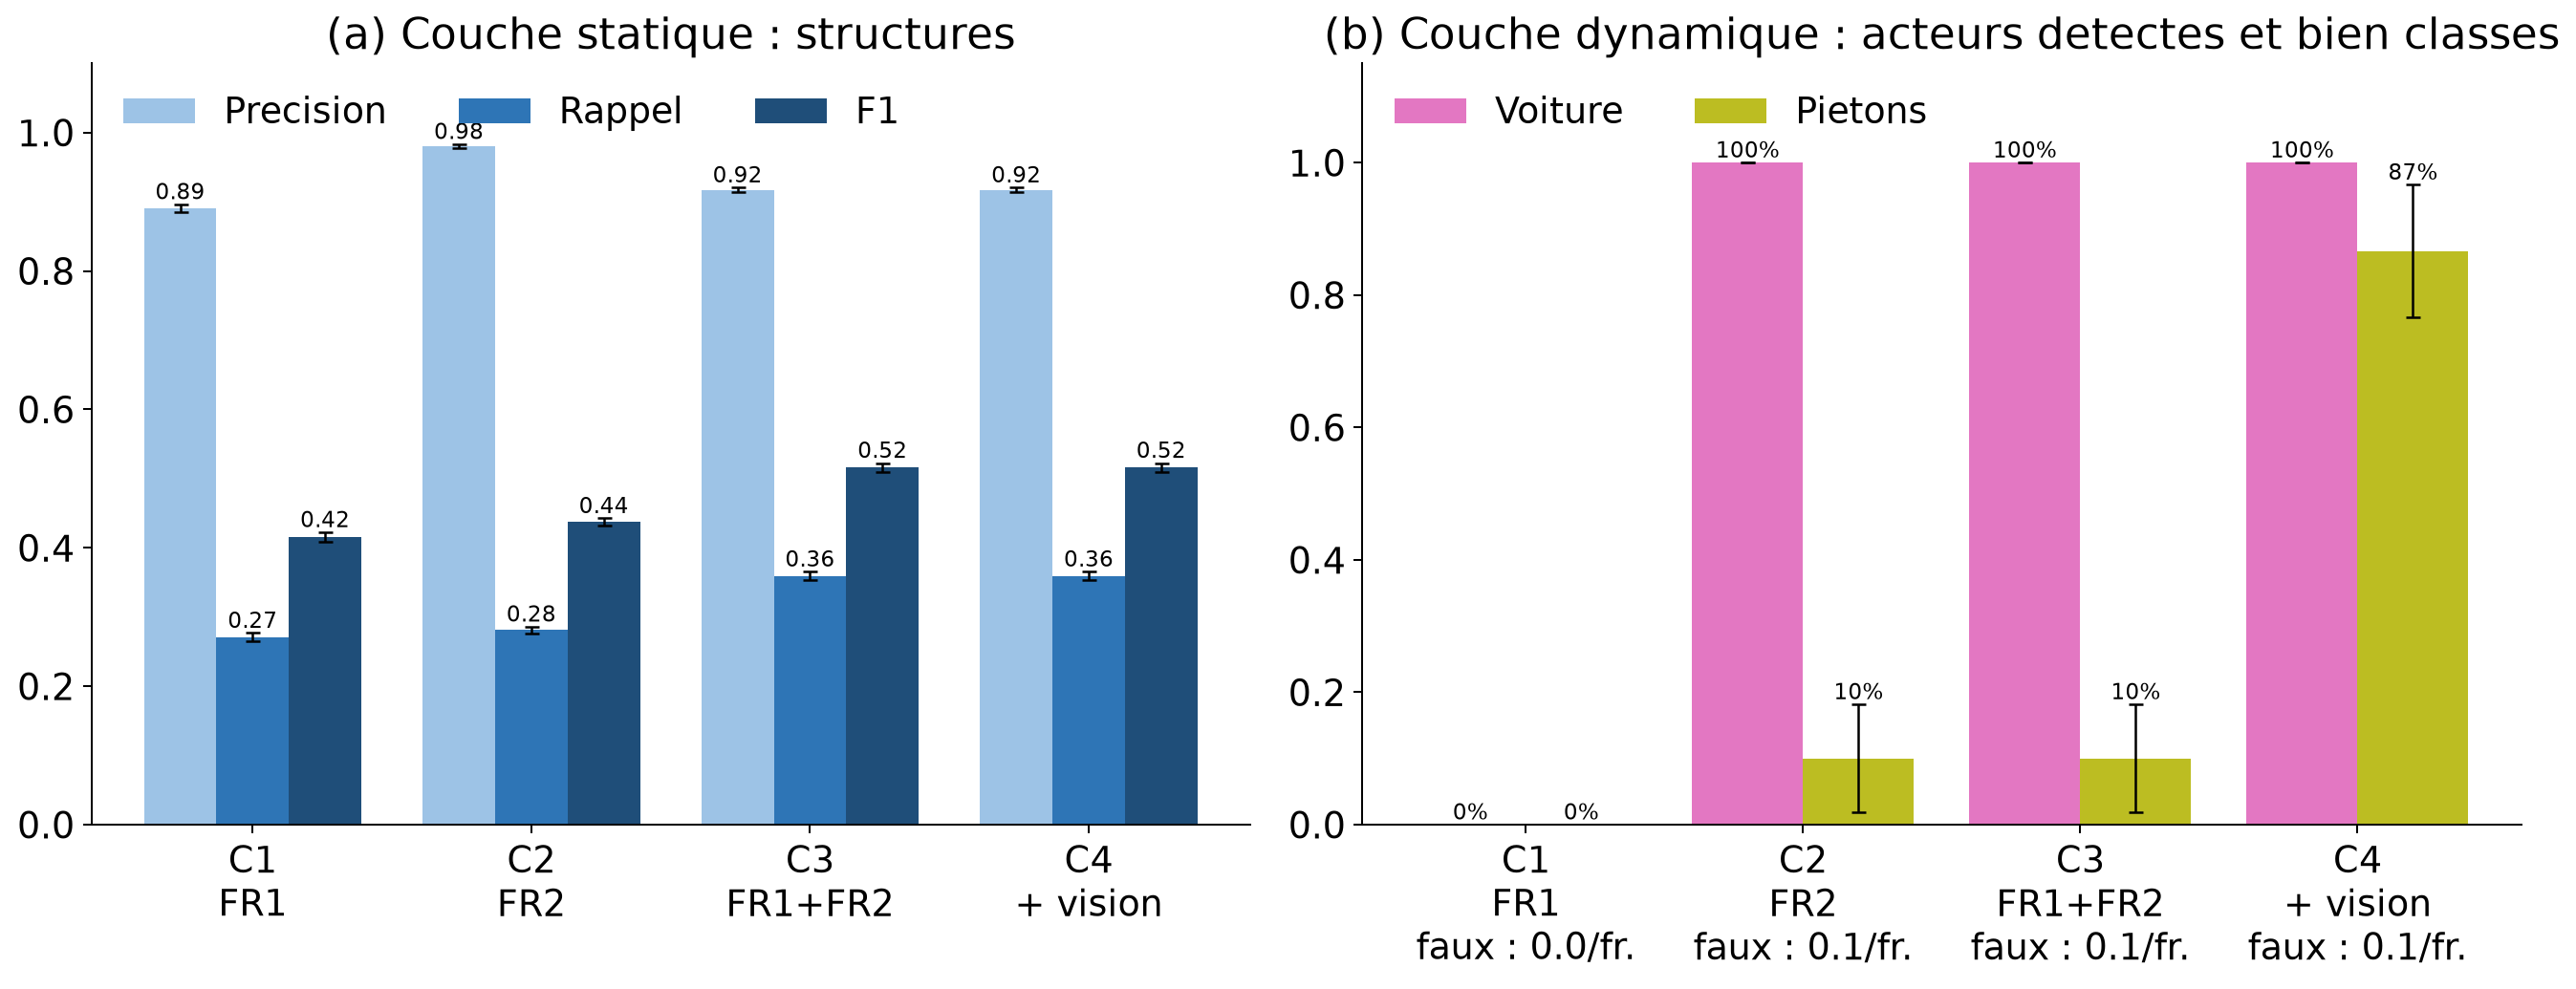
\includegraphics[width=\textwidth]{phase5/module3_metriques_configurations.png}
    \caption{Phase 5 : (a) précision, rappel et F1 de la couche statique (structures) ; (b) part des images où chaque acteur est retrouvé à moins de 3~m avec la bonne classe. Barres d'erreur : écart-type sur 10 tirages du bruit.}
    \label{fig:metriques_phase5}
\end{figure}

\begin{figure}[H]
    \centering
    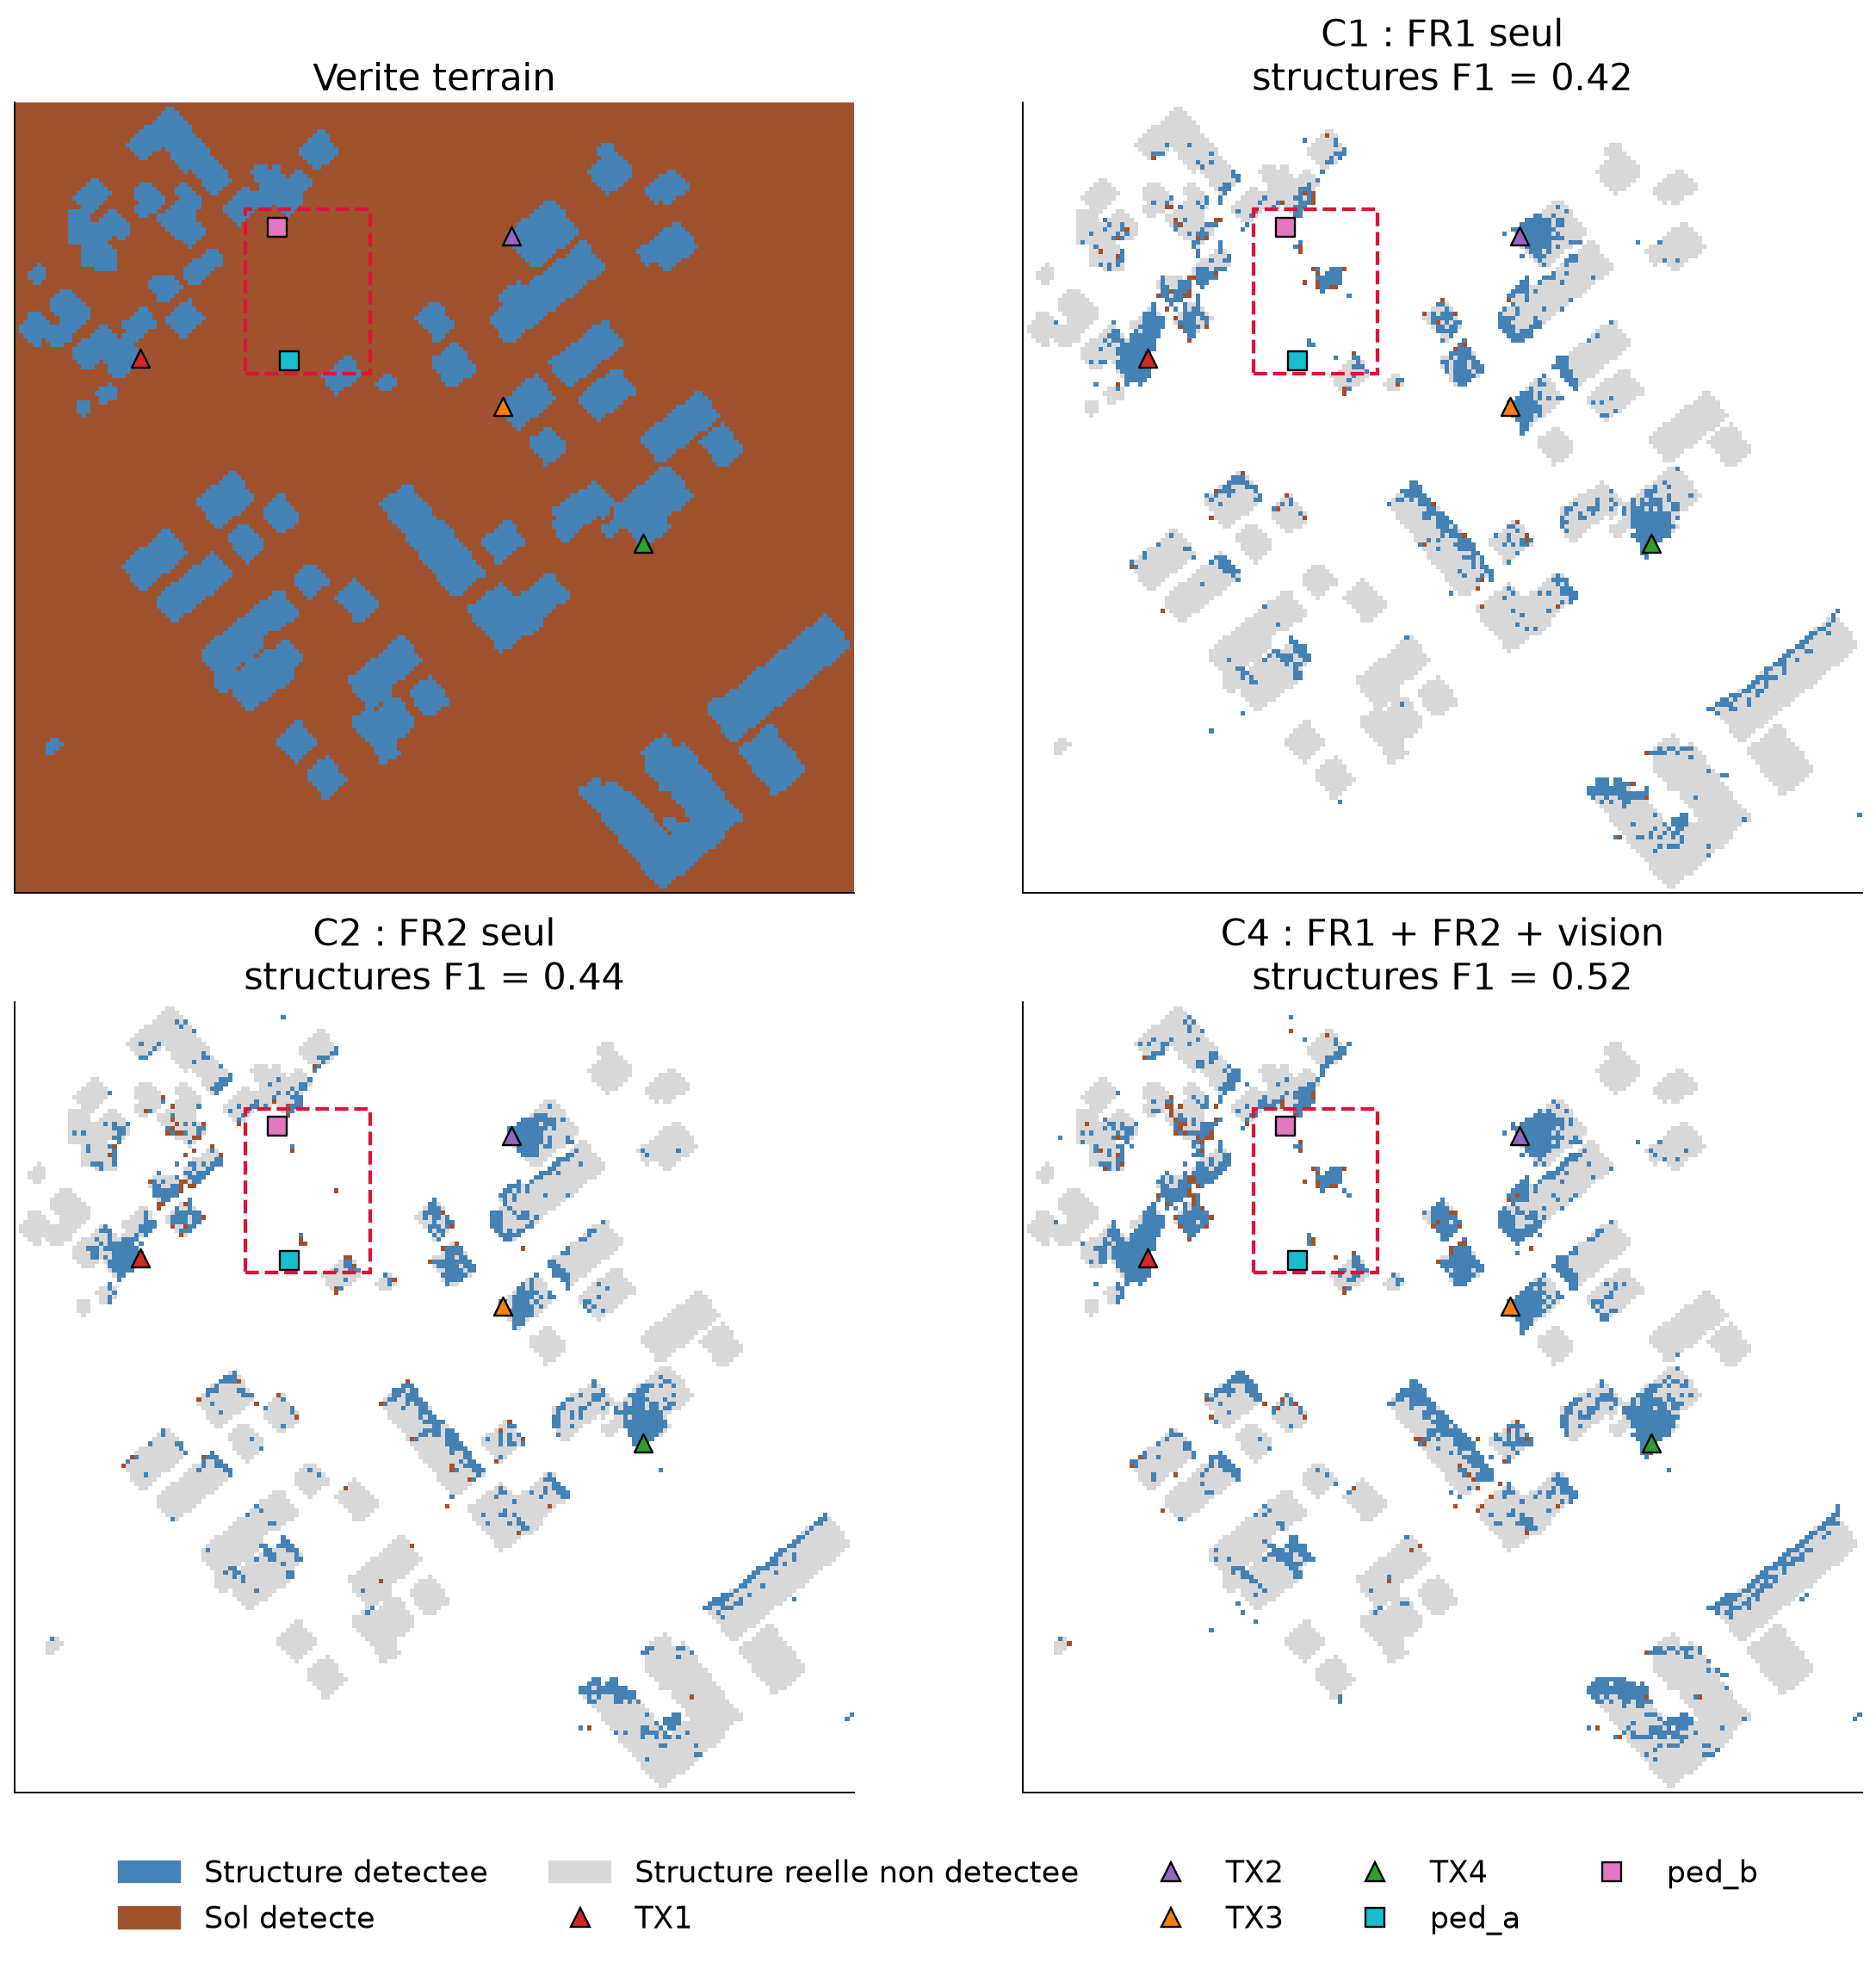
\includegraphics[width=\textwidth]{phase5/module3_jumeau_vues_dessus.png}
    \caption{Phase 5 : couche statique du jumeau, vue de dessus, comparée à la vérité terrain (en gris, les structures réelles non détectées). Le cadre rouge délimite la zone des acteurs, agrandie à la figure~\ref{fig:zoom_phase5}.}
    \label{fig:vues_phase5}
\end{figure}

\begin{figure}[H]
    \centering
    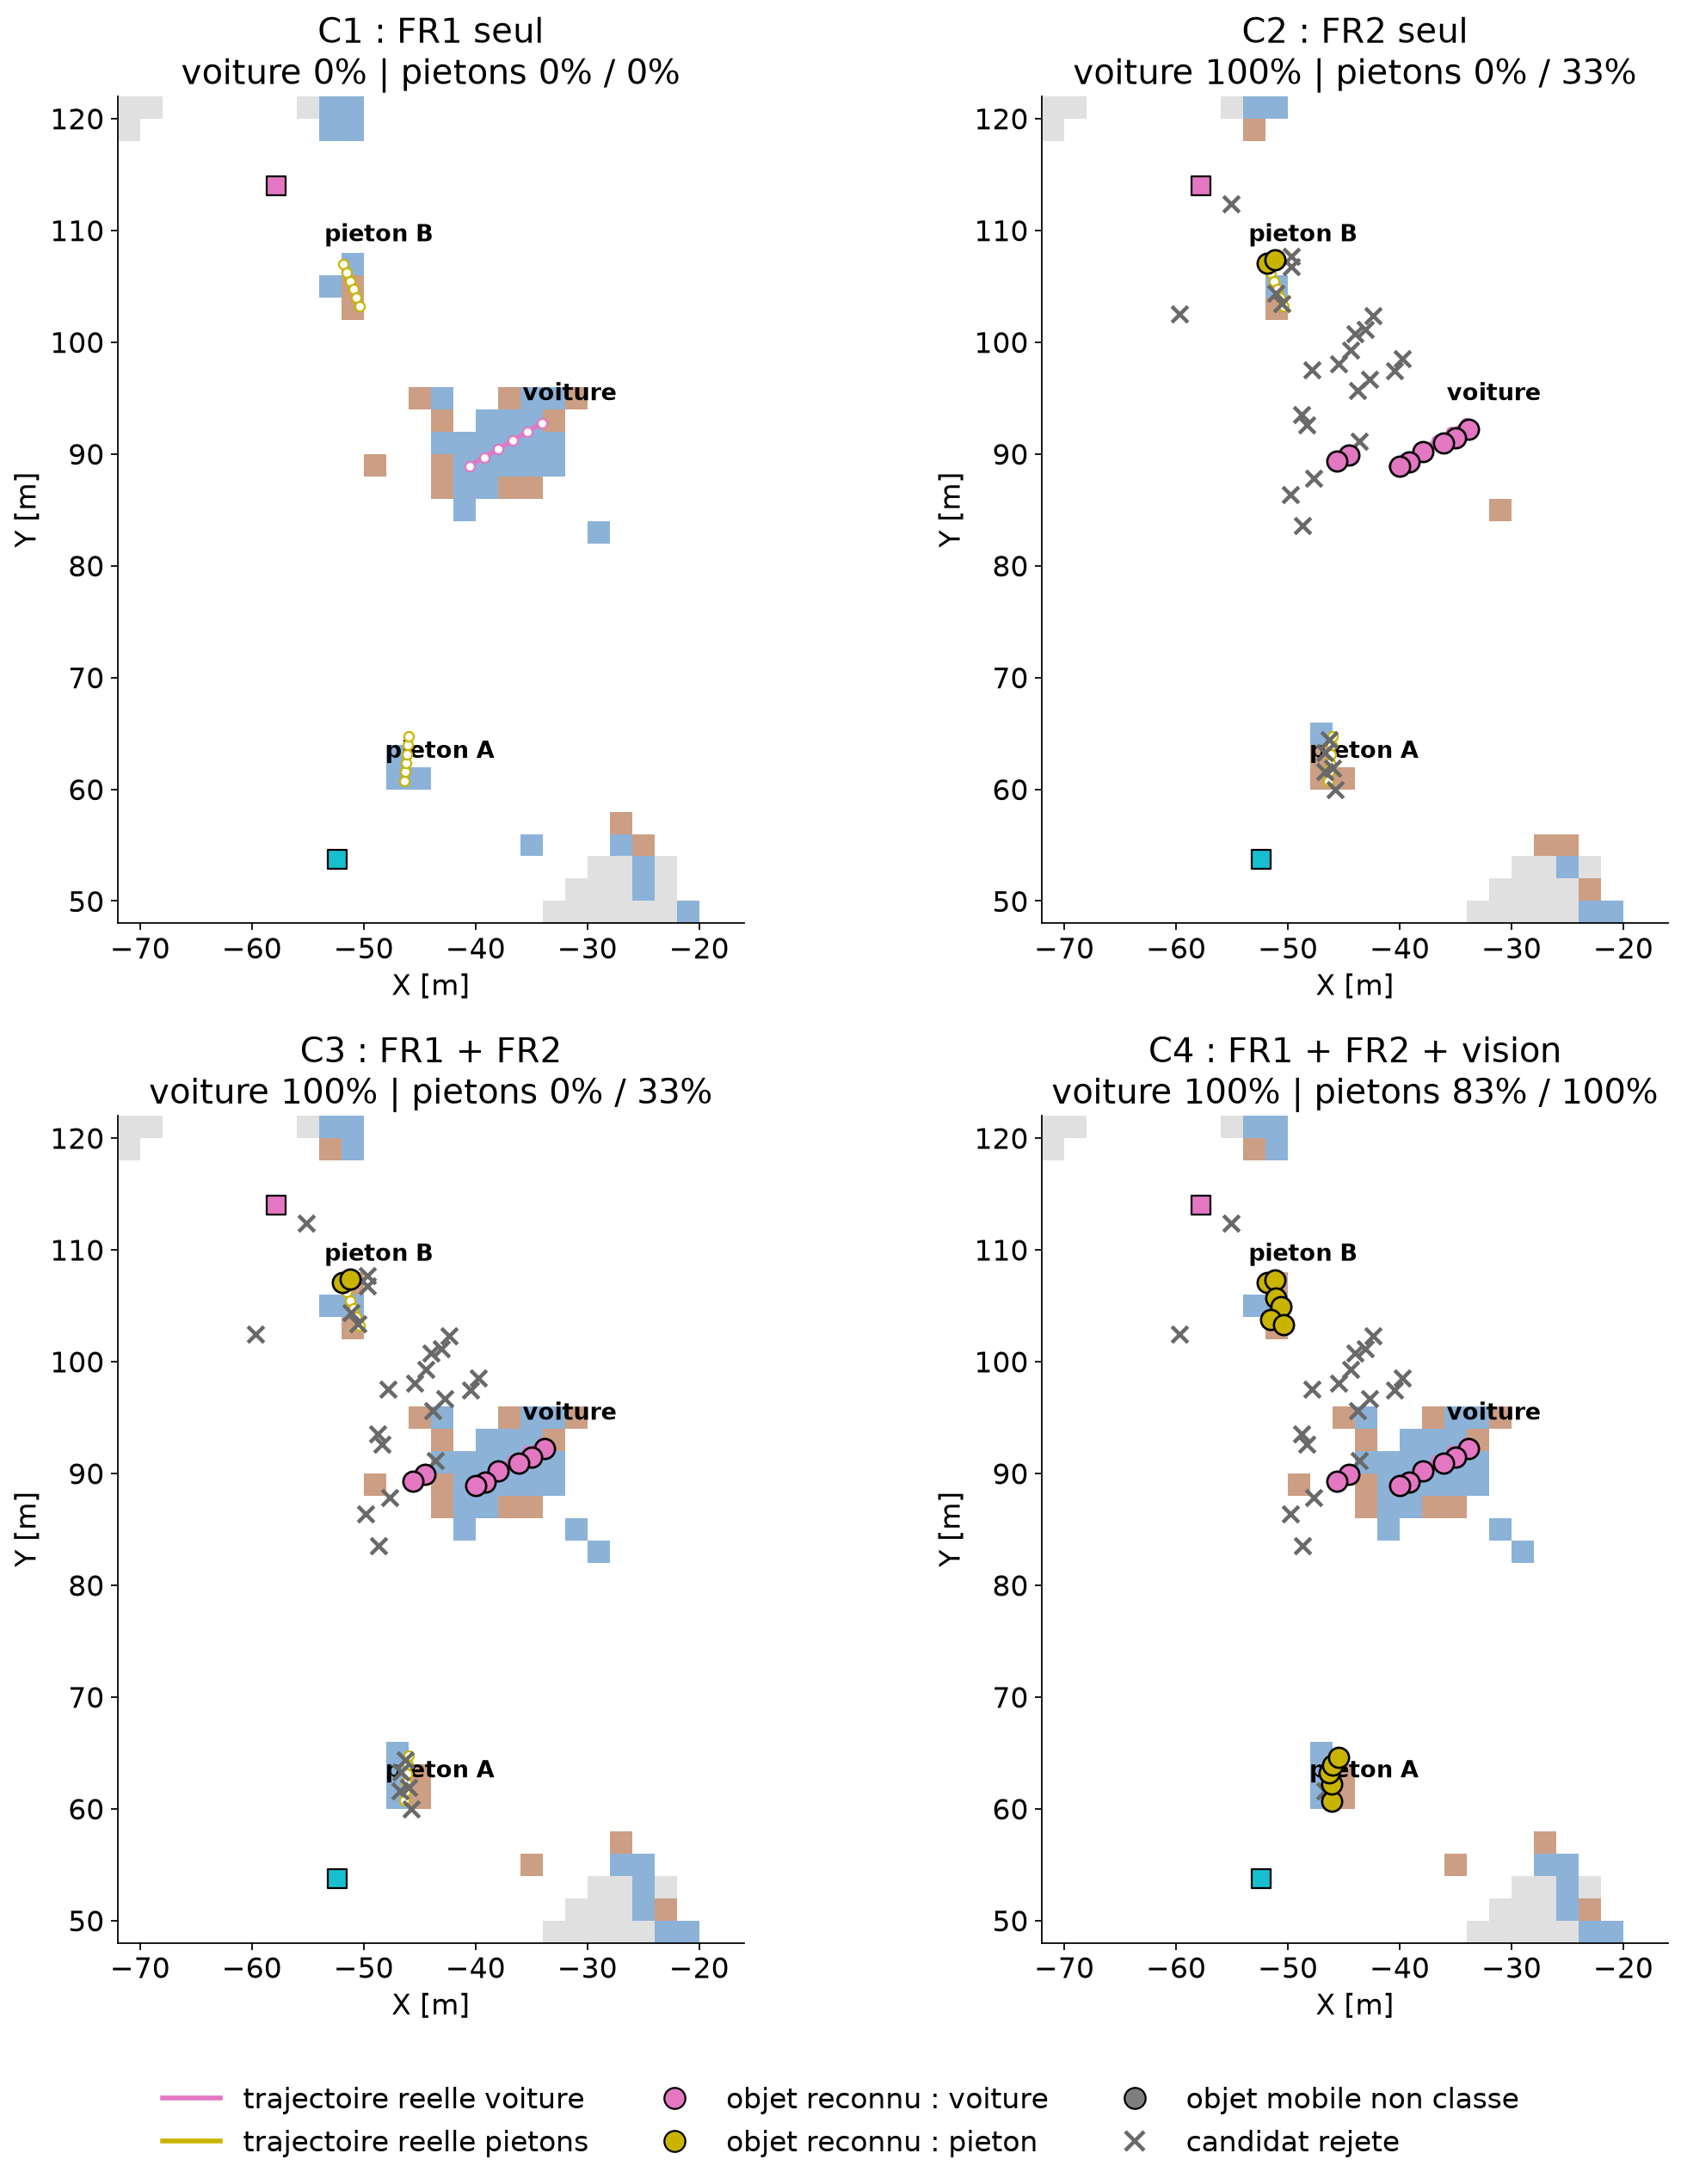
\includegraphics[width=0.92\textwidth]{phase5/module3_couche_dynamique_zoom.png}
    \caption{Phase 5 : zone des acteurs agrandie (tirage de référence). Lignes : trajectoires réelles sur les 6 images ; disques : objets retenus par le jumeau, colorés selon la classe reconnue ; croix : candidats rejetés par le filtre des points de vue. En fond, la couche statique de chaque configuration.}
    \label{fig:zoom_phase5}
\end{figure}

\subsubsection{Analyse de la couche statique}

\begin{itemize}[leftmargin=1.5em]
    \item \textbf{La précision est élevée partout (0,89 à 0,98).} Le filtre des deux récepteurs ne garde presque que de vraies surfaces, alors que près d'un tiers des échos passent par plusieurs rebonds. Avec des écarts-types inférieurs à 0,01, ces métriques, calculées sur des milliers d'échos, ne dépendent pas du tirage du bruit.
    \item \textbf{FR2 est la bande la plus précise} : 0,44~m d'erreur médiane et 12\,\% de points hors surface, contre 0,77~m et 27\,\% en FR1, grâce à sa meilleure résolution angulaire.
    \item \textbf{Le rappel est limité par la géométrie, pas par la mesure.} Quatre n\oe uds en toiture ne voient ni l'arrière des bâtiments, ni les cours, ni la plupart des toits : un bâtiment n'est cartographié que sur les façades tournées vers au moins deux n\oe uds (figure~\ref{fig:vues_phase5}).
    \item \textbf{La double bande augmente le rappel de 30\,\%} (de 0,27--0,28 à 0,36) et le F1 de 0,42--0,44 à 0,52. Une cellule doit être vue par deux récepteurs ; avec deux bandes, deux jeux d'échos indépendants atteignent les mêmes surfaces, et ce critère est plus souvent rempli. La précision baisse un peu (de 0,98 à 0,92), car les points moins précis de FR1 entrent dans la carte.
    \item \textbf{Le rappel du sol reste très faible (2 à 4\,\%)} : la vérité terrain contient tout le sol visible du ciel (environ 118\,000~m$^2$), alors qu'un radar en toiture ne reçoit d'écho du sol qu'à courte distance ; aux angles rasants, l'énergie part loin du récepteur.
    \item \textbf{Les échos FR1 des acteurs laissent de fausses structures} : une dizaine de voxels le long des trajectoires dès que FR1 est utilisé, contre un seul avec FR2 seul (figure~\ref{fig:zoom_phase5}, C1). Faute de Doppler suffisant, ces échos sont traités comme statiques. Une amélioration simple serait d'écarter les échos FR1 statiques situés là où FR2 voit un objet mobile.
\end{itemize}

\subsubsection{Analyse de la couche dynamique}

Le tableau~\ref{tab:frames_phase5} montre, pour la configuration C4 et le tirage de référence, comment chaque acteur est retrouvé à chaque image.

\begin{table}[H]
    \centering
    \caption{Configuration C4, tirage de référence : erreur de position et sources de chaque détection. R($k$) : échos radar reçus par $k$ récepteurs distincts ; V($k$) : objets créés par la vision depuis $k$ caméras.}
    \label{tab:frames_phase5}
    \begin{tabular}{cccc}
        \toprule
        \rowcolor{tabhead}
        \hd{Image} & \hd{Voiture} & \hd{Piéton A} & \hd{Piéton B} \\
        \midrule
        0 & 0,59~m --- R(3) & manqué --- R(1) seul & 0,11~m --- R(2) \\
        1 & 0,67~m --- R(3) & 0,91~m --- R(1) + V(1) & 1,12~m --- R(2) + V(1) \\
        2 & 0,61~m --- R(3) & 0,22~m --- R(1) + V(1) & 0,27~m --- R(1) + V(2) \\
        3 & 0,23~m --- R(3) & 0,17~m --- R(1) + V(3) & 0,38~m --- R(1) + V(2) \\
        4 & 0,45~m --- R(3) & 0,12~m --- R(1) + V(2) & 0,89~m --- R(1) + V(2) \\
        5 & 0,57~m --- R(3) & 0,59~m --- V(3) & 0,10~m --- R(2) + V(2) \\
        \bottomrule
    \end{tabular}
\end{table}

\begin{itemize}[leftmargin=1.5em]
    \item \textbf{La voiture est reconnue à 100\,\% dès que FR2 est utilisé}, avec 0,52~m d'erreur moyenne. À chaque image, 65 à 85 échos la confirment, reçus par TX1, TX2 et TX3, jamais par TX4, dont la vue sur les acteurs est masquée (comme l'avait montré sa caméra en phase~3). FR1 ne la détecte jamais comme mobile : son Doppler médian (45~Hz) reste sous la résolution de 100~Hz.
    \item \textbf{Avec le radar seul, les piétons sont presque perdus} : 0\,\% pour le piéton A, $20 \pm 16$\,\% pour le piéton B. Leurs rares échos (1 à 4 par image) ne sont presque toujours reçus que par un récepteur (TX2 pour A, TX3 pour B), et le filtre des fantômes les rejette. C'est le revers de ce filtre : il élimine les fantômes, mais aussi les cibles faibles vues d'un seul point de vue.
    \item \textbf{La vision apporte le point de vue qui manque.} Avec les objets qu'elle crée, les piétons sont reconnus dans $77 \pm 13$\,\% (A) et $97 \pm 7$\,\% (B) des images, avec 0,35 et 0,39~m d'erreur. Le tableau~\ref{tab:frames_phase5} le montre bien : presque toutes les détections de piétons combinent un seul récepteur radar et une à trois caméras. Le seul échec (piéton A, image 0) se produit quand la détection de la caméra a déjà servi à étiqueter l'unique écho radar : aucun objet vision indépendant n'est alors créé.
    \item \textbf{L'analyse a permis de corriger l'association radar-vision.} Dans une première version, les échos du piéton B étaient étiquetés « car » à l'image 0 : les caméras en toiture ne voyaient que la voiture, et le critère de la plus petite distance en pixels les favorisait. La distance relative et le contrôle de profondeur (\S\ref{subsec:etape4}) ont supprimé cette confusion, héritée de la méthode de la phase~3 : le piéton B n'est plus jamais pris pour une voiture.
    \item \textbf{Une caméra qui confirme un écho n'est pas un point de vue indépendant.} Nous avons essayé de la compter comme second point de vue : les fantômes de la voiture réapparaissent alors (1,5 faux objet par image), car la caméra, sur le même toit que le récepteur, voit le fantôme dans la même direction que lui.
    \item \textbf{Les faux objets sont rares} ($0{,}08 \pm 0{,}17$ par image). Le cas restant est un fantôme de la voiture, à environ 9~m, vu de façon cohérente par TX2 et TX3 aux images 1 et 2 : le filtre géométrique atteint sa limite quand deux récepteurs voient le même trajet multiple.
\end{itemize}

Les six critères de validation de la phase~5 sont remplis (\texttt{phase5\_summary.json}) : reconstruction exacte sans bruit, FR2 plus précis que FR1, séparation des cibles mobiles par Doppler en FR2, gain de la double bande sur les structures, gain des objets vision sur les piétons, et faux objets rares dans la configuration finale.

\subsection{Discussion transversale}
\label{subsec:discussion}

\textbf{Ce qui se retrouve d'une phase à l'autre.}
\begin{itemize}[leftmargin=1.5em]
    \item \emph{Les piétons sont la cible la plus difficile pour le radar}, quel que soit le modèle : 32 points contre 305 pour la voiture en phase~3, et 0 à 20\,\% de reconnaissance avec le radar seul en phase~5, où leurs rares échos ne sont souvent vus que par un récepteur. Dans les deux cas, c'est la vision qui les rend visibles dans la carte, ce qui justifie la fusion radar-vision au c\oe ur du projet.
    \item \emph{TX4 est mal placé pour cette scène.} Sa caméra est masquée (phase~3), il fournit le moins de points radar (3\,622) et la carte partielle la moins fidèle (similarité 0,519, phase~4), et il ne confirme jamais la voiture en phase~5. Le déplacer serait plus utile que d'ajouter un n\oe ud.
    \item \emph{La comparaison des bandes mène à la double bande.} FR1 l'emporte sur la portée aux phases~3 et~4 (22\,\% d'échos en plus, surtout sur le sol et les façades éloignées) ; FR2 l'emporte sur la précision dès que les mesures sont réalistes (phase~5) ; et les deux ensemble couvrent plus de structures que chacune séparément (\S\ref{subsec:choix_bande}).
    \item \emph{Un modèle plus réaliste change les chiffres, pas les conclusions.} Passer des points idéalisés des phases~3 et~4 aux mesures réalistes de la phase~5 fait apparaître des fantômes (environ 30\,\% des échos) et des erreurs de position (0,4 à 0,8~m), que le filtre des points de vue maîtrise. Les grandes tendances restent les mêmes : la voiture est bien mieux perçue par le radar que les piétons, et c'est la vision qui permet de reconnaître ces derniers.
\end{itemize}

\textbf{Limites de l'évaluation.} Tous nos résultats viennent de la simulation : matériaux ITU, scène OpenStreetMap simplifiée, images synthétiques. Le mAP du détecteur est mesuré sur le même type de rendus que son entraînement et ne dit rien de son comportement sur des images réelles. Enfin, l'évaluation porte sur un seul scénario (trois acteurs, six images). Les tirages du bruit de la phase~5 montrent que les métriques sont stables vis-à-vis du bruit, mais pas vis-à-vis d'autres scènes ou trajectoires : ce serait la prochaine étape de validation.

\subsection{Synthèse des résultats}

\begin{table}[H]
    \centering
    \caption{Synthèse des résultats obtenus.}
    \begin{tabularx}{\textwidth}{F{3.8cm}L}
        \toprule
        \rowcolor{tabhead}
        \hd{Module} & \hd{Résultat principal} \\
        \midrule
        1a. Acquisition ISAC & Chaîne Sionna RT validée à 3,5~GHz (6 liaisons BS--UE, CIR, PDP) ; nuage radar multistatique à 28~GHz avec seuil de détection (16\,784 points retenus sur 20\,896) \\
        1b + 2. Acquisition vision et fusion & 305 points voiture et 32 points piéton étiquetés (100\,\% des points \texttt{target}, aucune contamination), détecteur YOLOv8n mAP50~$=0{,}965$, fusion active sur les 6 images ; à bilan de liaison identique, 28~GHz retient 18\,\% de points en moins que 3,5~GHz \\
        3. Cartographie sémantique & Grille bayésienne 3D (1\,396 cellules observées), encodage HD validé (requête correcte, compression $\times10\,454$), fusion HD multi-BS limitée au-delà de 2 ou 3 n\oe uds \\
        Phase 5. Jumeau numérique double bande & Mesures radar réalistes (retard + angle d'arrivée, fantômes), classes par Doppler et hauteur ; FR1 + FR2 + vision : structures F1~$=0{,}52$ (précision 0,92), voiture 100\,\%, piétons 77--97\,\%, 0,08 faux objet par image (moyennes sur 10 tirages) \\
        \bottomrule
    \end{tabularx}
\end{table}

% ============================================================
\section{Limitations et Périmètre du Projet}
\label{sec:limitations}
% ============================================================

Cette section rassemble les écarts entre ce que nous avons réalisé et l'architecture visée (\S\ref{sec:architecture_proposee}), avec leur justification.

\begin{itemize}[leftmargin=1.5em]
    \item \textbf{Fréquence porteuse} : à partir de la phase~3, chaque phase a été menée à 3,5~GHz et à 28~GHz, et nous avons retenu la double bande (\S\ref{subsec:choix_bande}). La validation du simulateur (phase~2, \S\ref{subsec:res_phase2}) n'a été faite qu'à 3,5~GHz. Le sol de la scène des phases~3 à~5 a les propriétés du béton, car \texttt{itu\_very\_dry\_ground} n'est pas défini au-delà de 10~GHz.
    \item \textbf{Hypothèses du seuil de détection} : le bilan de liaison (tableau~\ref{tab:bilan_liaison}), commun aux phases~3 à~5, repose sur des valeurs typiques et non mesurées, sans étude de sensibilité. Une intégration plus longue ou un $\mathrm{SNR}_{\min}$ plus bas augmenteraient le nombre de points retenus ; une puissance plus faible ou un bruit plus élevé le réduiraient, surtout à 28~GHz, où le seuil retire déjà 20\,\% des trajets, contre 2\,\% à 3,5~GHz.
    \item \textbf{Hauteur des stations de base} : le plan prévoyait 10~m, mais les quatre n\oe uds sont en toiture (18 à 23~m environ), pour garantir une vue directe sur les acteurs. C'est un déploiement en toiture courant dans les réseaux réels.
    \item \textbf{Piétons peu visibles au radar} : 32 points contre 305 pour la voiture en phase~3 (\S\ref{subsec:res_phase3}), et 0 à 20\,\% de reconnaissance avec le radar seul en phase~5. Les objets créés par la vision compensent en grande partie (77 à 97\,\% de reconnaissance, \S\ref{subsec:res_phase5}), mais l'identification des piétons repose alors surtout sur la vision.
    \item \textbf{Couverture du jumeau numérique} : le rappel des structures (0,36) est limité par les faces que les n\oe uds en toiture ne voient pas, et celui du sol (4\,\%) par leur hauteur (\S\ref{subsec:res_phase5}). Les échos FR1 des acteurs, non reconnus comme mobiles, laissent quelques fausses structures le long des trajectoires. Enfin, l'échantillonnage des réflexions diffuses sur GPU fait légèrement varier les résultats d'une exécution à l'autre, sans changer les conclusions.
    \item \textbf{TX4 sans confirmation vision} : sa caméra est masquée par un bâtiment au premier plan (\S\ref{subsec:res_phase3}). C'est une contrainte de site réaliste plutôt qu'une erreur de conception.
    \item \textbf{Fusion multi-BS par addition HD} : au-delà de 2 ou 3 n\oe uds, elle ne fait plus mieux que le meilleur n\oe ud seul (\S\ref{subsec:res_phase4}). Cette limite de la superposition bipolaire ne concerne que la démonstration de compression, pas la grille bayésienne.
    \item \textbf{Suivi temporel} : l'association radar-vision est refaite indépendamment à chaque image (\S\ref{subsec:art_tracking}). Nous n'avons pas implémenté de filtre de suivi complet (Kalman, JPDA), la séquence testée ne comptant que 6 images ; la phase~5 ajoute seulement une confirmation des objets d'une image à la suivante.
    \item \textbf{Pas de segmentation} : le module 1b (\S\ref{subsec:pipeline_six_modules}) prévoyait YOLOv8-seg \textit{ou} SegFormer. Nous n'avons utilisé que YOLOv8n en mode détection, car la fusion n'a besoin que des boîtes (\S\ref{sec:choix_tech}).
    \item \textbf{Modules 4 à 6} (carte de risque, JSCC, apprentissage fédéré, interface avec le modèle du monde AGI, \S\ref{subsec:pipeline_six_modules}) : leurs interfaces sont définies dans l'architecture, mais ils exploitent la carte au lieu de la construire. Nous les avons laissés hors du périmètre de ce rapport, centré sur la construction et la validation de la carte (modules 1a, 1b, 2 et 3). Ils font l'objet de la phase~6 de la feuille de route (tableau~\ref{tab:feuille_route}).
\end{itemize}

% ============================================================
\section{Conclusion Générale}
\label{sec:conclusion}
% ============================================================

Ce rapport a présenté le projet SDM-VA-ISAC, de la revue de littérature aux résultats. Les deux architectures de référence, le \textit{Telecom Brain} et SA-VA-ISAC (\S\ref{sec:etat_art}), laissent ouverte une question : comment passer des signaux physiques à une représentation sémantique de l'environnement. Notre architecture en six modules (\S\ref{sec:architecture_proposee}) y répond, et nous en avons implémenté et évalué la partie perception et cartographie (modules 1a, 1b, 2 et 3) : une simulation Sionna RT d'un vrai quartier, une chaîne de perception à six n\oe uds qui fusionne ISAC et vision par KD-tree, et une carte sémantique 3D compressée par encodage hyperdimensionnel.

Nous avons comparé chaque choix technologique important à ses alternatives (\S\ref{sec:choix_tech}), et analysé les limites rencontrées : occultation de TX4, capacité de la fusion HD au-delà de 2 ou 3 n\oe uds, hauteur des antennes, absence de suivi temporel complet (\S\ref{sec:limitations}).

La bande de fréquence a été choisie sur mesures : à partir de la phase~3, chaque étape a été exécutée à 3,5~GHz et à 28~GHz, avec le même bilan de liaison. FR1 apporte la portée, FR2 la précision ; nous avons retenu la double bande, qui combine les deux.

La phase~5 transforme cette chaîne en un jumeau numérique ISAC double bande, construit à partir de mesures radar réalistes (retard et angle d'arrivée, fantômes de trajets multiples, classes tirées du Doppler et de la hauteur et non du matériau) et évalué par rapport à la géométrie réelle de la scène. Elle montre que FR1 et FR2 se complètent : FR2 est plus précis et seul capable de séparer les cibles lentes par le Doppler, et les deux bandes ensemble couvrent davantage de structures. Elle montre aussi que la vision, quand elle peut créer ses propres objets, compense ce que le radar ne voit pas : les piétons, presque perdus par le radar seul, sont reconnus dans 77 à 97\,\% des images. L'analyse des résultats nous a enfin permis de corriger deux défauts de l'association radar-vision hérités de la phase~3.

La carte sémantique 3D, et en particulier sa version compressée par encodage hyperdimensionnel, fournit ainsi le lien entre couche physique et représentation sémantique qui manquait dans la littérature. Elle peut servir directement aux modules 4 à 6 (carte de risque, compression JSCC, interface avec un modèle du monde causal), qui ne sont pas nécessaires pour clore le présent travail.

\subsection*{Feuille de route et travaux à venir}

Le plan de travail initial comptait six phases. Nous y avons inséré le jumeau numérique ISAC double bande comme phase~5, car il fallait une carte réaliste et évaluée avant d'y ajouter les modules d'optimisation ; les deux dernières phases du plan initial deviennent donc les phases~6 et~7 (tableau~\ref{tab:feuille_route}).

\begin{table}[H]
    \centering
    \caption{Plan de travail du projet SDM-VA-ISAC, mis à jour avec la phase de jumeau numérique.}
    \label{tab:feuille_route}
    \begin{tabularx}{\textwidth}{>{\centering\arraybackslash}p{1.6cm}LL>{\centering\arraybackslash}p{2.1cm}}
        \toprule
        \rowcolor{tabhead}
        \hd{Phase} & \hd{Tâches} & \hd{Livrables} & \hd{Statut} \\
        \midrule
        Phase 1 & Revue de littérature IEEE JSAC/TWC 2023--2025 & État de l'art, lacunes identifiées (\S\ref{sec:etat_art}) & Terminée \\
        Phase 2 & Scène Blender/OSM $\to$ XML, calibration Sionna RT & Environnement simulé fonctionnel (\S\ref{subsec:res_phase2}) & Terminée \\
        Phase 3 & YOLOv8/SegFormer + fusion KDTree + Sionna sensing & Pipeline de perception multimodal (\S\ref{subsec:res_phase3}) & Terminée \\
        Phase 4 & Grille bayésienne 3D, encodage HD, visualisation Open3D & Carte sémantique interactive (\S\ref{subsec:res_phase4}) & Terminée \\
        Phase 5 \newline \footnotesize(ajoutée) & Jumeau numérique ISAC double bande : mesures radar réalistes, FR1 + FR2, objets créés par la vision, évaluation par vérité terrain & Jumeau numérique évalué (\S\ref{subsec:res_phase5}) & Terminée \\
        \choix Phase 6 & Risk heatmap, JSCC, complétion par diffusion, \textit{beamforming} informé & Modules d'optimisation intégrés & À venir \\
        \choix Phase 7 & Métriques (mIoU, $\tau_{\text{map}}$, $\Delta_{\text{VA}}$, $\rho$), \textit{baselines} & Résultats quantitatifs + graphes & À venir \\
        \bottomrule
    \end{tabularx}
\end{table}

Par rapport au plan initial, la phase~3 n'a utilisé que YOLOv8 (sans SegFormer, \S\ref{sec:limitations}), et la phase~5 réalise déjà une partie de l'évaluation prévue en phase~7 : vérité terrain, comparaison avec l'ISAC seul et premier gain dû à la vision.

La phase~6 s'appuiera sur le jumeau numérique : sa couche dynamique (positions et classes des acteurs) alimentera la carte de risque et le \textit{beamforming} informé, et sa couche statique indiquera les zones masquées que la complétion par diffusion devra reconstruire. La phase~7 pourra réutiliser la vérité terrain et le protocole d'évaluation de la phase~5 (tirages multiples, configurations comparées) pour mesurer toutes les métriques du cadre d'évaluation (\S\ref{subsec:cadre_evaluation}).

\newpage
% ============================================================
%  RÉFÉRENCES
% ============================================================
\begin{thebibliography}{99}

\bibitem{saad2025}
W. Saad \textit{et al.},
``Artificial General Intelligence (AGI)-Native Wireless Systems: A Journey Beyond 6G,''
\textit{arXiv preprint}, 2025.

\bibitem{sa_va_isac_main}
Y.~Lu, W.~Mao, H.~Du, O.~A.~Dobre, D.~Niyato, Z.~Ding,
``Semantic-Aware Vision-Assisted Integrated Sensing and Communication: Architecture and Resource Allocation,''
\textit{IEEE Wireless Communications}, vol.~31, no.~3, pp.~302--308, juin 2024.

\bibitem{shannon1948}
C. E. Shannon,
``A Mathematical Theory of Communication,''
\textit{Bell System Technical Journal}, vol.~27, pp.~379--423, 1948.

\bibitem{pearl2009}
J. Pearl,
\textit{Causality: Models, Reasoning and Inference}, 2nd ed.
Cambridge University Press, 2009.

\bibitem{isac_survey}
F.~Liu \textit{et al.},
``Integrated Sensing and Communications: Toward Dual-Functional Wireless Networks for 6G and Beyond,''
\textit{IEEE JSAC}, vol.~40, no.~6, pp.~1728--1767, 2022.

\bibitem{semantic_comm}
H.~Xie \textit{et al.},
``Deep Learning Enabled Semantic Communication Systems,''
\textit{IEEE Trans. Signal Process.}, vol.~69, pp.~2663--2675, 2021.

\bibitem{drl_beamforming}
W.~Cui, K.~Shen, W.~Yu,
``Spatial Deep Learning for Wireless Scheduling,''
\textit{IEEE JSAC}, vol.~37, no.~6, pp.~1248--1261, 2019.

\bibitem{vision_isac}
Y. Gao \textit{et al.},
``Vision-Aided ISAC in Low-Altitude Economy Networks via De-Diffused Visual Priors,''
\textit{arXiv:2507.01574}, 2025.

\bibitem{cell_free_mimo}
Ö.~T.~Demir, E.~Björnson, L.~Sanguinetti,
``Foundations of User-Centric Cell-Free Massive MIMO,''
\textit{Found. Trends Signal Process.}, vol.~14, no.~3--4, pp.~162--472, 2021.

\bibitem{federated_learning}
H.~B.~McMahan \textit{et al.},
``Communication-Efficient Learning of Deep Networks from Decentralized Data,''
in \textit{Proc. AISTATS}, 2017, pp.~1273--1282.

\bibitem{sionna_rt_2}
J. Hoydis \textit{et al.},
``Sionna RT: Differentiable Ray Tracing for Radio Propagation Modeling,''
\textit{arXiv:2303.11103}, 2023.

\bibitem{sionna}
J. Hoydis \textit{et al.},
``Sionna: An Open-Source Library for Next-Generation Physical Layer Research,''
\textit{arXiv:2203.11854}, 2022.

\bibitem{remcom_wi}
Remcom Inc.,
``Wireless InSite Propagation Software --- User's Manual,'' 2023.

\bibitem{ultralytics_yolov8}
G. Jocher, A. Chaurasia, J. Qiu,
``Ultralytics YOLOv8,''
\url{https://github.com/ultralytics/ultralytics}, 2023.

\bibitem{segformer}
E. Xie, W. Wang, Z. Yu, A. Anandkumar, J. M. Alvarez, P. Luo,
``SegFormer: Simple and Efficient Design for Semantic Segmentation with Transformers,''
in \textit{Proc. NeurIPS}, 2021.

\bibitem{domain_randomization}
J. Tobin, R. Fong, A. Ray, J. Schneider, W. Zaremba, P. Abbeel,
``Domain Randomization for Transferring Deep Neural Networks from Simulation to the Real World,''
in \textit{Proc. IROS}, 2017.

\bibitem{bar_shalom_tracking}
Y. Bar-Shalom, T. E. Fortmann,
``Tracking and Data Association,''
Academic Press, 1988.

\bibitem{bentley_kdtree}
J. L. Bentley,
``Multidimensional Binary Search Trees Used for Associative Searching,''
\textit{Communications of the ACM}, vol.~18, no.~9, pp.~509--517, 1975.

\bibitem{elfes_occupancy}
A. Elfes,
``Using Occupancy Grids for Mobile Robot Perception and Navigation,''
\textit{IEEE Computer}, vol.~22, no.~6, pp.~46--57, 1989.

\bibitem{thrun_occupancy}
S. Thrun,
``Learning Occupancy Grid Maps with Forward Sensor Models,''
\textit{Autonomous Robots}, vol.~15, pp.~111--127, 2003.

\bibitem{grieves_digital_twin}
M. Grieves, J. Vickers,
``Digital Twin: Mitigating Unpredictable, Undesirable Emergent Behavior in Complex Systems,''
in \textit{Transdisciplinary Perspectives on Complex Systems}, Springer, 2017.

\bibitem{kanerva_hdc}
P. Kanerva,
``Hyperdimensional Computing: An Introduction to Computing in Distributed Representation with High-Dimensional Random Vectors,''
\textit{Cognitive Computation}, vol.~1, pp.~139--159, 2009.

\bibitem{plate_hrr}
T. A. Plate,
``Holographic Reduced Representations,''
\textit{IEEE Trans. Neural Networks}, vol.~6, no.~3, pp.~623--641, 1995.

\bibitem{rahimi_hdc}
A. Rahimi, P. Kanerva, J. M. Rabaey,
``A Robust and Energy-Efficient Classifier Using Brain-Inspired Hyperdimensional Computing,''
in \textit{Proc. ISLPED}, 2016.

\bibitem{open3d}
Q.-Y. Zhou, J. Park, V. Koltun,
``Open3D: A Modern Library for 3D Data Processing,''
\textit{arXiv:1801.09847}, 2018.

\end{thebibliography}

\end{document}
